\documentclass[a4paper,twoside,openright]{book}

\usepackage[T1]{fontenc}
\usepackage[utf8x]{inputenc}

\usepackage{lmodern}

\usepackage[francais]{babel}

\usepackage{array}
\usepackage{mathtools}
\usepackage{amssymb}
\usepackage{amsthm}
\usepackage{mathtools}
\usepackage{makeidx}
\usepackage{graphicx}
\usepackage{url}
\usepackage{epigraph}
\usepackage{hyperref}
\usepackage{natbib}

\usepackage{fancyhdr}
\pagestyle{fancy}

\usepackage{hyperref}

\usepackage{type1cm}
\usepackage{lettrine}

\usepackage{color}
\usepackage{colortbl}
\usepackage{placeins}

\usepackage{tikz}
\usepackage{tikz-qtree}


% Setup pdf meta-data.
\hypersetup{ % Modifiez la valeur des champs suivants
pdfauthor = {Thomas Moulard},
pdftitle = {Optimisation num\'erique pour la robotique et ex\'ecution de trajectoires r\'ef\'erenc\'ees capteurs},
pdfsubject = {Optimisation num\'erique pour la robotique et ex\'ecution de trajectoires r\'ef\'erenc\'ees capteurs},
pdfkeywords = {optimisation numérique, typage, type, robotique, humano\"ide},
pdfcreator = {Thomas Moulard},
pdfproducer = {Thomas Moulard}
}


% Please fancyhdr.
\setlength{\headheight}{25pt}

% Customize chapter head.
\makeatletter
\renewcommand\chapter{\if@openright\cleardoublepage\else\clearpage\fi
                    \thispagestyle{empty}%
                    \global\@topnum\z@
                    \@afterindentfalse
                    \secdef\@chapter\@schapter}
\def\@makechapterhead#1{%
  \vspace*{50\p@}%
  {\parindent \z@ \raggedright \normalfont
    \ifnum \c@secnumdepth >\m@ne
      \if@mainmatter
        \huge\bfseries\thechapter\enspace
      \fi
    \fi
    \Huge \bfseries #1\par\nobreak
    \vskip 40\p@
  }}
\makeatother

% Add definition definition.
\newtheorem{mydef}{Définition}
\newtheorem{myexample}{Exemple}

% Enforce math style.
\everymath{\displaystyle}

% Generate index.
\makeindex

% Custom commands.
\newcommand{\transformation}[2]{%
\ensuremath{{}^{#1}\!\text{M}_{#2}}}

\begin{document}
\bibliographystyle{plainnat}
%
\author{Thomas Moulard}
\title{Optimisation numérique pour la robotique et exécution de trajectoires référencées capteurs}
\date{Juillet 2012}
\maketitle
%
\frontmatter
\tableofcontents{\thispagestyle{fancy}}
%
\mainmatter 
\chapter{Introduction}
\label{chap:intro}

\epigraph{Text text text text text text text text text text text text
  text text text text text text text text text text text text text
  text text text text text text text text text text text text text
  text text text text text text text text text text text text text
  text text text text}{Some Author}
\clearpage


\section{Les enjeux de la robotique}

\subsection{50 ans de robotique mobile}
\subsection{De la voiture autonome à l'assistance aux personnes âgées}

\section{Robotique humanoïde: l'enfance...}

\subsection{...d'un domaine scientifique...}
\subsection{...et d'un secteur industriel}

\subsection{Le projet japonais HRP}

\section{Présent et futur de la robotique}


\chapter[Optimisation]{Optimisation et généricité}
\label{chap:roboptim}

\epigraph{Text text text text text text text text text text text text
  text text text text text text text text text text text text text
  text text text text text text text text text text text text text
  text text text text text text text text text text text text text
  text text text text}{Some Author}
\clearpage

\section[Optimisation]{Optimisation numérique et robotique}

\subsection{Introduction à l'optimisation numérique}

\lettrine[lines=2, lraise=0.1, nindent=0em, slope=-.5em]%
{L}{a} robotique s'appuie sur différents outils mathématiques
pour résoudre les problèmes auxquels elle se trouve confrontée. Parmi
ces outils, l'optimisation numérique figure à une place de choix.


L'optimisation numérique est une branche des mathématiques permettant
de choisir automatiquement la meilleure solution parmi un ensemble de
solutions possibles. Les applications possibles couvrent des domaines
variés de la recherche opérationnelle aux statistiques et bien sûr la
robotique. Dans ce domaine particulier, l'optimisation numérique
permets par exemple d'optimiser un mouvement pour en améliorer
certains caractéristiques ou bien encore trouver la prochaine commande
à envoyer aux moteurs du robot afin de réaliser une tâche donnée.



Résoudre un problème d'optimisation numérique signifie trouver les
meilleurs paramètres solutionnant le problème. Par meilleurs, il faut
entendre les paramètres minimisant la valeur d'une fonction de
coût. Intuitivement, on peut se représenter cette fonction comme un
indicateur de la ``qualité'' de la solution trouvée. Une solution
présentant un coût fort sera donc peu satisfaisante tandis qu'une
solution présentant un coût faible sera, elle, très attrayante. Tout
le raisonnement est ensuite fondé sur la linéarité -- au moins locale!
-- de cette fonction de coût. Plus simplement, près d'une mauvaise
solution, il n'y aura que des solutions légèrement meilleures et
légèrement pires, mais jamais trop différentes. De ce fait, il
``suffit'' de chercher dans quelle direction aller pour se diriger
vers les meilleurs solutions pour finir par les trouver. Cette
approche implique une limitation majeure: si la fonction de coût n'est
pas convexe, on ne trouvera pas forcément la meilleure solution
globale -- parmi toutes les solutions -- mais ma meilleure solution
locale. C'est à dire qu'au voisinage de cette solution, toutes les
autres solutions sont de moins bonnes qualités. Dans cette situation,
tous les solveurs arrêtent leur recherche, mais rien ne garantit
qu'ailleurs il n'existe pas une autre solution de meilleure qualité.


Ce raisonnement permets de trouver les meilleurs paramètres pour un
problème donné, mais il est rare qu'une fonction de coût seule puisse
capturer complètement un problème donné. En fonctionnant de manière
indépendante du problème sous-jacent, on confère aux solveurs une
grande polyvalence. Mais par là même, il devient nécessaire
d'expliciter sous quelles conditions une solution au problème donné
est acceptable. Prenons un exemple: pour aller d'un point $A$ à un
point $B$ le plus rapidement possible, se déplacer avec une vitesse
infinie est sans aucun doute la solution optimale. Cependant, une
telle réponse ne présente guère d'intérêt dans la mesure où aucun
système physique ne sera en mesure de l'exécuter.


Deux stratégies peuvent alors être choisies. La première est
d'exprimer directement dans la fonction de coût cette information
supplémentaire. Dans le cadre de l'exemple précédemment cité, on
pourrait concevoir une fonction de coût réalisant la somme du temps de
déplacement et de la vitesse moyenne du robot. De ce fait, une vitesse
trop grande pénalise le résultat et par ce biais, le solveur tentera
plutôt de transformer la trajectoire géométrique plutôt que de jouer
sur la vitesse de déplacement du système. La limite de cette approche
est simple à comprendre: au fur et à mesure que les biais s'accumulent
-- le plus souvent en sommant les uns aux autres --, le coût initial
peut se retrouver ignoré par le solveur car numériquement
négligeable. La fonction de coût n'a alors plus aucune justification
physique et ses variations peuvent devenir de plus en plus difficiles
à analyser pour le solveur.  Une seconde solution consiste à ajouter
des contraintes au problème. Ces contraintes sont exprimées sous la
forme d'équations ou d'inéquations déterminant si une solution donnée
est une solution acceptable. En robotique, des contraintes très
courantes sont les bornes sur les butées articulaires. Il est rare sur
un robot que les axes puissent bouger de manière totalement libre. De
ce fait, il est courant d'ajouter des contraintes inégalités
spécifiant que tel ou tel valeur de joint doit rester dans un
intervalle donné.


En exprimant comment résoudre un problème pratique via la construction
d'une fonction de coût $f$ et de contraintes $g_i > 0$,
\textbf{modélise} le problème afin qu'il soit soluble par optimisation
numérique. Ce procédé n'est pas trivial car la qualité de la
modélisation impacte lourdement à la fois les temps de calcul et la
qualité du résultat final.



\subsection{Modélisation mathématique d'un problème}


Résoudre un problème d'optimisation revient à trouver une solution pour:

\begin{equation}
  \min_{\mathbf{x} \in \mathbb{R}^n} f(x) \text{ sous la contrainte } \mathbf{x} \in \mathbf{X}
\end{equation}

où $f : \mathbb{R}^n \mapsto \mathbb{R}$ est la fonction de coût et
$\mathbf{X} \subset \mathbb{R}^n$ est l'espace des solutions
admissibles. Cet espace est habituellement défini par un ensemble de
contraintes égalités et inégalités:

\begin{equation}
  \mathbf{X} \equiv \left\{
  \begin{array}{l l}
    c_i (x) = 0    & \quad i \in \xi \\
    c_j (x) \leq 0 & \quad j \in \nu \\
  \end{array} \right.
\end{equation}

$c_i$, $c_j$ sont respectivement les ensembles de contraintes égalités
et inégalités. $i$ et $j$ des indices identifiant les contraintes.


L'optimisation numérique a pour objectif de développer des stratégies
-- algorithmes -- pouvant déterminer $\mathbf{x} \in \mathbf{X}$
minimisant les valeurs de la fonction $f$.


En absence d'arguments fort tel que la convexité de $f$ ainsi que des
contraintes $c_i, i \in \xi \cup \nu$, la solution $\mathbf{x}$
fournie par le solveur peut être un minimum local \index{minimum
  local}.


En effet, la plupart des méthodes d'optimisation tentent de trouver un
minimum en raffinant itérativement une solution à partir d'un candidat
initial $\mathbf{x_{\text{init}}} \in \mathbf{X}$. Le solveur, dès
lors, nécessite un critère d'arrêt à ce processus itératif. Ce critère
est donné par les conditions de Karush-Kuhn-Tucker \index{conditions
  de Karush-Kuhn-Tucker} ou conditions KKT.

\begin{mydef}\label{def:chap1_kkt}
Si $\mathbf{x} \in \mathbf{X}$ est un minimum local, alors il existe
$\lambda_i, i \in \xi$ et $\mu_j, j \in \nu$ des constantes non-nulles
appelées multiplicateurs KKT tels que:
%
\begin{description}
\item[\textbf{Critère de stabilité}] \begin{equation}
  \nabla f(x) + \sum_{i \in \xi} \lambda_i c_i(x) + \sum_{j \in \nu} \mu_i c_i(x) = 0
\end{equation}
\item[\textbf{Critère de faisabilité primale}] \begin{equation}
\left\{
\begin{array}{l l}
  c_i (x) = 0    & \quad i \in \xi \\
  c_j (x) \leq 0 & \quad j \in \nu \\
\end{array} \right.
\end{equation}
\item[\textbf{Critère de faisabilité duale}] \begin{equation}
\mu_j \geq 0, j \in \nu
\end{equation}
\item[\textbf{Critère de complémentarité}] \begin{equation}
\mu_j c_j(x) = 0, j \in \nu
\end{equation}
\end{description}
\end{mydef}

Il est à noter que la Définition~\ref{def:chap1_kkt} fournit des
conditions suffisantes afin de déterminer si un point est un minimum
local. Sous conditions de régularité, et dans le cas où le problème
est convexe, les conditions KKT sont nécessaires et suffisantes.


\subsection{Zoologie des solveurs}

\subsubsection{Zoologie mathématique}


Au-delà de cette présentation de la théorie générale, on peut
regrouper les techniques de résolutions en différentes catégories
selon la difficulté des problèmes pouvant être traités. Nous ne nous
attarderons ici que sur les techniques d'optimisation
continues. Différentes caractéristiques peuvent rendre la résolution
plus délicate:
%
\begin{itemize}
\item Présence de contraintes,
\item Non-convexité de la fonction de coût ou des contraintes,
\item Non-linéarité de la fonction de coût ou des contraintes,
\item Fonction non -- ou mal -- définie en dehors des contraintes,
\item Variations numériques fortes entraînant des erreurs numériques
  difficiles à juguler,
\item etc.
\end{itemize}
%
La combinaison de ces difficultés entraînent la classification des
solveurs dans de très nombreuses catégories dont un extrait est
détaillé dans le Tableau~\ref{tbl:chap1_solver}.
%
\begin{table}\label{tbl:chap1_solver}
\begin{center}
\begin{tabular}{|>{\small}p{.24\textwidth}|>{\small}p{.305\textwidth}|>{\small}p{.305\textwidth}|}
\hline
\textit{Classe de problème} & \textit{Fonction de coût} & \textit{Contraintes}\\
\hline
\textbf{Moindres carrés linéaires} & $\sum_{i \in \{1, 2, \dotsc, n\}} (r_i - \mathbf{x}_i)^2$ où les $r_i$ sont des constantes & non \\
\hline
\textbf{LQP} \small{(opt. quadratique linéaire)} & quadratique & linéaire \\
\hline
\textbf{SQP} \small{(opt. non-linéaire)} & non-linéaire & non-linéaire \\
\hline
\end{tabular}
\end{center}
\caption{Zoologie des problèmes en optimisation numérique.}
\end{table}
%
Les algorithmes de résolution ont également des particularités
intrinsèques qui peuvent être particulièrement intéressantes dans le
cadre de la robotique. Par exemple, le démarrage à chaud ou ``warm
start'' \index{démarrage à chaud} \index{warm start|see{démarrage à
  chaud}} est la possibilité, pour un solveur, de pouvoir résoudre
plusieurs problèmes à la suite tout en se souvenant de son état
interne afin de pouvoir gagner en temps de calcul lorsque le nouveau
problème est très proche du problème précédemment résolu. Cette
situation intervient notamment lorsque l'on optimise une trajectoire
tout en l'exécutant. L'optimisation se déroule pour différents
instants proches dans le temps pour lesquels l'évolution de l'état du
robot est minime. Une autre caractéristique est la capacité, pour un
solveur, de pouvoir être interrompu à n'importe quelle itération tout
en garantissant que la solution actuelle, bien qu'incomplète,
respecte la totalité des contraintes du problème. Ce comportement est
important lorsque l'optimisation est lancée dans un contexte où les
contraintes temporelles sont fortes, telle que dans le contrôleur
calculant les commandes du robot.



\subsubsection{Zoologie logicielle}


On l'aura compris: d'une théorie unique découle un ensemble
d'algorithmes pouvant résoudre des problèmes de complexité
variée. Plaçons nous désormais à la place d'un roboticien devant
résoudre un problème particulier. Quels logiciels peut-il utiliser
pour se faire? Le Tableau~\ref{tbl:chap1_soft} détaille une partie
des paquets logiciels existants.
%
\begin{table}\label{tbl:chap1_soft}
\begin{center}
\begin{tabular}{|p{.24\textwidth}|p{.305\textwidth}|p{.305\textwidth}|}
\hline
\textit{Logiciel} & \textit{Classe de problème} & \textit{Caractéristiques}\\
\hline
\textbf{\href{http://devernay.free.fr/hacks/cminpack/index.html}{C/C++ MinPack}} & Moindres carrés linéaires & C/C++, réentrant, thread-safe \\
\hline
\textbf{\href{https://projects.coin-or.org/Ipopt}{Coin IPOPT}} & SQP & C++, réentrant \\
\hline
\textbf{\href{http://www.aemdesign.com/}{CFSQP}} & SQP & C, réentrant \\
\hline
\end{tabular}
\end{center}
\caption{Zoologie des problèmes en optimisation numérique.}
\end{table}
%
Une conclusion s'impose au regard de cette liste de paquets logiciels:
les techniques les plus compliquées à implémenter sont peu disponibles
et il n'existe pas d'outil unifié permettant de résoudre différents
types de problèmes. Enfin, chaque outil traite une catégorie de
problème en particulier. Il est raisonnable de se demander si chaque
utilisateur, lorsqu'il commence à définir son problème est à même de
choisir de manière pertinente le solveur -- et donc le framework --
adapté à son problème. Est-il certain que toutes les fonctions seront
différentiables et continues deux fois? une fois? Est-on certain de ne
pas avoir besoin de contraintes inégalités, voire de ne pas avoir
besoin du tout de contraintes? Rien n'est moins sûr. Un exemple simple
est la gestion des collisions. On peut tout à fait développer un outil
robotique et le faire fonctionner dans un environnement ouvert avant
de vouloir s'attaquer à un problème plus difficile et prendre en
compte les collisions. Cela peut poser des problèmes extrêmement
important car le solveur ne sera pas le même dans les deux
cas. Cependant, il semble qu'avoir à réécrire, ou tout du moins
adapter, le problème précédent à un nouvelle bibliothèque logicielle
est inutile puisque finalement les deux problèmes se formalisent au
sein d'un même paradigme.


\section{De la dif\-ficulté à passer d'un paradigme uni\-que à une implémentation unifiée}


A première vue, il pourrait sembler que l'absence d'une architecture
unifiée pour la résolution de problèmes d'optimisation numérique est
le simple résultat d'un manque de volonté et/ou de coordination entre
développeurs. Nous allons montrer ici qu'il n'en est rien. Une simple
agglomération des implémentations de différentes stratégies de
résolution ne saurait donner un ensemble cohérent et performant en
terme de temps de calcul sans une véritable réflexion sur comment
modéliser le paradigme décrit à la section précédente tout en prenant
en compte les limites internes des langages de programmation. Nous
allons tout particulièrement nous intéresser à la programmation
orientée objet qui est la fondation d'une large proportion des
langages modernes.


\subsection{Typage, programmation orienté objet et familles de types}

\subsubsection{$\lambda$-calcul et théorie des types}

Lors du développement de l'informatique, les langages de programmation
ont tout d'abord été de simples outils permettant de représenter du
code machine de manière succincte et plus facilement lisible par les
humains. Cependant, avec la complexification croissante des
applications informatiques, vérifier la correction des programmes est
rapidement devenu un enjeu critique. Pour se faire, les langages de
programmation ont progressivement adopté le typage comme moyen de
n'autoriser que la construction de programmes valides. Cette notion de
type a issue de la théorie des types \index{théorie des types}, une
branche de la logique mathématique. La première théorie unifiée des
types a été développée par Bertrand Russel \index{Bertrand Russel} au
début du vingtième siècle dans les \emph{Principia
  Mathematica}~\citep{pm}.


Afin de démontrer les difficultés que peuvent poser la modélisation
d'un problème d'optimisation numérique, nous allons nous appuyer sur
un système de calcul formel particulier, le $\lambda$-calcul
\index{$\lambda$-calcul} inventé par Alonzo Church \index{Alonzo Church}
dans les années trente. Ce système de calcul formel a une expressivité
équivalente à une \index{Machine de Türing}. Nous allons tout d'abord
nous concentrer sur la construction des lambda-termes
\index{lambda-terme}, c'est à dire l'ensemble des expressions
syntaxiquement correcte pouvant être construite en lambda-calcul. Ces
lambda-termes peuvent être divisés en trois catégories: variables,
applications et abstractions. Les variables: $x$, $y$, \ldots Les
applications sont l'ensemble des expressions $u v$ où $u$ et $v$ sont
deux lambda-termes. Enfin les abstractions sont les expressions du
type: $\lambda x.u$ où $x$ est une variable et $u$ un
lambda-terme. Par exemple, l'application identité peut s'écrire en
lambda-calcul: $\lambda x.x$.


La procédure qui, à partir de n'importe quel lambda-terme, tente de la
simplifier en réalisant les applications par réécriture est appelé
$\beta$-conversion \index{$\beta$-conversion}. En réduisant un
lambda-terme, on réalise le calcul associé à ce dernier. Une propriété
utile serait de pouvoir déterminer si toutes les lambda-réductions
terminent, c'est à dire que l'on peut réduire tous les lambda-termes
jusqu'à un point où plus aucune réécriture \index{réécriture} n'est
possible.


Hélas, ce n'est pas le cas en lambda-calcul. Soit:

\begin{eqnarray}
  \Delta \equiv \lambda x.x\\
  \Omega \equiv \Delta \Delta \equiv (\lambda x.x) (\lambda x.x)
\end{eqnarray}

 On peut remarquer que la $\beta$-reduction de $\Omega$ boucle
 indéfiniment:

\begin{equation}
  (\lambda x.x) (\lambda x.x) =_{\beta} (\lambda x.x) (\lambda x.x)
\end{equation}

En terme calculatoire, on peut considérer que ce programme boucle et
ne termine jamais.


Face à ce constat, une autre interrogation se pose: peut-on construire
un sous-ensemble des lambda-termes normalisables? La réponse est oui,
via l'utilisation du lambda-calcul simplement typé
\index{lambda-calcul simplement typé}. Dans cette version du
lambda-calcul, toute expression est annotée par un type. Les types
sont de deux sortes: $\iota$ et $\tau_1 \rightarrow \tau_2$ à
condition que $\tau_1$ et $\tau_2$ soient des types. $\iota$
représente le(s) type(s) primitif(s) du langage permettant de
représenter les booléens ou un sous-ensemble des nombres entiers ou
réels par exemple. Si $x$ est de type $\iota$, on a alors:
%
\begin{equation}
  x \vdash \iota
\end{equation}
%
\ldots prononcé ``$\iota$ type $x$''. L'ensemble des types est quand à
lui noté $\Gamma$.


En définissant des règles de typage appropriée, on peut restreindre
les lambda-termes bien typés aux lambda-termes
normalisables. Cependant, une limitation de cette approche est qu'une
grande partie des expressions que l'on souhaiterait construire ne sont
pas correctement typés. En particulier, il n'est pas possible de
construire la fonction exponentielle dans ce paradigme.


\subsubsection{Programmation orienté objet et typage}

Indépendamment des systèmes de calculs formels, divers modèles plus
pratiques ont été développé au cours de la seconde moitié du vingtième
siècle. Notamment, la programmation orienté objet \index{programmation
  orienté objet} a été introduite par Ole-Johan Dahl \index{Ole-Johan
  Dahl} et Kristen Nygaard \index{Kristen Nygaard} dans \index{Simula
  I} au cours des années soixante. Ce langage avait pour but de
permettre le développement de simulation à événements discrets. Ce
paradigme de pensée s'est progressivement développé jusqu'à être
massivement adopté par la majorité des langages de programmation au
cours des années quatre-vingt dix. L'adoption massive du C++ (Bjarne
Stroustrup \index{Bjarne Stroustrup}, 1983) a participé à la
démocratisation de la POO.


La POO introduit la classe comme élément unitaire permettant la
conception d'un programme informatique. Alors qu'auparavant, une
séparation stricte était observée entre les données et les
algorithmes, une classe est un élément du langage regroupant à ces
deux éléments. Les algorithmes fournit par une classe sont alors
appelés ``méthodes'' tandis que les données prennent le nom
``d'attributs''. Cette réunification des données et des traitements
sur les données s'inscrit pleinement dans la lignée de la vision
informatique introduite par Von Neumann et l'architecture portant son
nom. L'innovation clé de cette architecture a été de permettre la
transmission sur un même bus des instructions composant un programme
ainsi que des données sur lesquelles les instructions vont
s'appliquer. On peut donc dire que la classe a poussé la réunification
algorithmes/données jusqu'à la conception interne des logiciels.

\begin{mydef}\label{def:chap1_type}
  Un type peut soit être un type fondamental noté $\iota$, soit un
  type fonctionnel, soit un type de classe. En pratique, il existe
  plusieurs types fondamentaux: réels, entiers, booléens mais le
  nombre de types de base ne change en rien les règles de typage.
\end{mydef}

\begin{mydef}\label{def:chap1_class}
  Soit $\tau$ un type de classe. $\tau$ est défini par $a \in \mathfrak{A}_\tau$
  l'ensemble des attributs -- données -- de la classe et $m \in
  \mathfrak{M}_\tau$ l'ensemble des méthodes de la classe.

  \emph{Notation:} on notera $\tau.a$ l'attribut $a$ de la classe $\tau$ et
  $\tau.m$ la méthode $m$ de la classe $\tau$. Afin d'éviter les ambiguïtés,
  l'ensemble des symboles composant les éléments $\mathfrak{A}_\tau$ et
  $\mathfrak{M}_\tau$ sont disjoints.
\end{mydef}

\begin{mydef}\label{def:chap1_method}
  Soit $\mathfrak{M}_\tau$ l'ensemble des méthodes d'une classe. Une
  méthode $m$ du type de classe $\tau$ est une variable de type $\tau
  \rightarrow \tau'$ où $\tau'$ est un type quelconque.

  \emph{Notation:} L'application de la méthode $m$ de la classe $\tau$
  devrait s'écrire $a.m \tau$ où $a \vdash \tau$. Dans la mesure où
  l'on sait que $m \in \mathfrak{M}_\tau$, on peut se passer
  d'appliquer explicitement le premier argument du type fonctionnel et
  directement écrire $\tau.m$ pour signifier l'application de la
  méthode $m$.
\end{mydef}

\begin{mydef}\label{def:chap1_attribute}
  Soit $\mathfrak{A}_\tau$ l'ensemble des attributs d'une classe. Un
  attribut $a$ du type de classe $\tau$ est une variable de type
  $\tau'$ quelconque à l'exception des types fonctionnels prenant un
  type $\tau$ en argument.
\end{mydef}


\begin{myexample}\label{ex:chap1_class}
  Soit $A$ une classe définie par:

  \begin{equation}
    A \equiv \{ \underbrace{\{ \text{foo} \vdash \iota
      \}}_{\text{attribut}}, \underbrace{\{ \text{bar} \vdash A
      \Rightarrow \iota, \text{baz} \vdash A \rightarrow \iota
      \}}_{\text{méthodes}} \}
  \end{equation}

  $A$ possède un attribut et deux arguments. D'après la définition de
  $A$ et les
  Définitions~\ref{def:chap1_method}~et~\ref{def:chap1_attribute}, on
  a:

  \begin{equation}
    a \vdash A \Rightarrow a.\text{foo} \vdash \iota
  \end{equation}

  \begin{equation}
    a \vdash A \Rightarrow a.\text{bar} \vdash A \rightarrow \iota
  \end{equation}
\end{myexample}


Cette représentation permet de pouvoir offrir une vue d'ensemble
intégrant à la fois des données structurées et l'ensemble des
opérations possibles sur ces dernières. Auparavant, la séparation de
ces deux éléments rendait plus difficile la construction d'une vision
globale: on ne pouvait, par définition, pas connaître la liste des
opérations définies sur un groupe de données. Soit $\tau$ un type de
classe, l'ensemble des fonctions prenant $\tau$ en entrée n'est pas
connu lors de la compilation car il peut être augmenté à tout moment
d'un nouvel élément en définissant une nouvelle routine. Il convient
donc de documenter la liste des opérations disponibles.

Inversement, il est souvent nécessaire d'augmenter le comportement
d'une classe en y ajoutant de nouvelles données et/ou de nouveaux
algorithmes. La POO modélise ce processus au travers de l'héritage de
classe. Soit $\tau_1$ un type de classe, $\tau_2$ un type de classe
héritant de $\tau_1$. On dit également que $\tau_2$ est un sous-type
de $\tau_1$, et est noté sous la forme:

\begin{equation}
  \tau_2 <: \tau_1
\end{equation}
%
%
Cette notion, proche de celle d'inclusion en théorie des ensembles,
permet de définir des familles de types interchangeables.
%
%
\begin{mydef}\label{chap1_oo_app}
  Soit $\Gamma$ un contexte de type. $\tau_1$, $\tau_2$, $\tau_3$
  trois types appartenant à ce contexte. La règle de typage des
  applications en programmation orienté objet est alors:


  \begin{equation}
    u~v~\text{bien formé} \Rightarrow u \vdash \tau_1 \rightarrow
    \tau_2 \wedge \tau_3 <: \tau_1
  \end{equation}

  Dès lors que $tau_3$ est un sous-type de $\tau_1$, les fonctions
  prenant en argument une variable de type $\tau_1$ acceptent
  également les arguments de type $\tau_3$.
\end{mydef}
%
\begin{mydef}\label{chap1_method_typing}
  Soit $\Gamma$ un contexte de type. $\tau_1$, $\tau_2$ deux types.

  On dit que $\tau_2 <: \tau_1$ si et seulement si:

  \begin{equation}
    \tau_2 <: \tau_1 \Leftrightarrow \mathfrak{A_{\tau_1}} \subset
    \mathfrak{A_{\tau_2}} \wedge \mathfrak{M_{\tau_1}} \subset
    \mathfrak{M_{\tau_2}}
  \end{equation}
\end{mydef}
%
Un sous-type se doit de contenir au moins tous les attributs et
méthodes de la classe dont elle hérite afin d'interdire la réécriture
vers des termes syntaxiquement faux. Le ``principe de substitution de
Liskov''\index{principe de substitution de
  Liskov}~\citep{Liskov94familyvalues} définit, de manière équivalente,
la relation de sous-typage sous l'énoncé suivant:
%
\begin{mydef}\label{chap1_liskov}
  Si $q(x)$ est une propriété démontrable pour tout objet $x$ de type
  $T$, alors $q(y)$ est vraie pour tout objet $y$ de type $S$ tel que
  $S$ est un sous-type de $T$.
\end{mydef}


La Définition~\ref{chap1_method_typing} introduit implicitement la
notion de polymorphisme d'héritage\index{polymorphisme!polymorphisme
  d'héritage}. Le polymorphisme\index{polymorphisme} est la capacité
pour un type fonctionnel de ne pas accepter en entrée un type unique,
mais une famille de types. Le polymorphisme le plus simple pouvant
être défini est la surcharge\index{surcharge}. Ce mécanisme autorise
la création de fonctions se réécrivant vers des $\lambda$-termes
différents selon le type de l'argument d'entrée. La formalisation de
ce système est décrit dans~\citep{Castagna95acalculus}.

Une autre forme de polymorphisme est le polymorphisme d'héritage. Si
$\tau_1$ et $\tau_2$ sont deux types tels que $\tau_2 <: \tau_1$ et
qu'il existe une méthode $m$ dans $\tau_1$ et $\tau_2$, alors tout
application de la méthode $m$ à un objet de type $\tau_2$ se réécrira
vers le $\lambda$-terme $\tau_2.m$. Un sous-type peut donc fournir une
réécriture alternative d'une fonction afin d'en spécialiser le
comportement.

La généralisation de cette propriété à toutes les fonctions au lieu
des méthodes uniquement permets d'obtenir le ``multiple
dispatch''~\citep{Muschevici2008}. Ce mécanisme est disponible dans
un nombre assez limité de langages de programmation dont Common
Lisp. En effet, contrairement à la surcharge, le multiple dispatch
ainsi que le polymorphisme d'héritage nécessite une résolution à
l'exécution qui peut pénaliser l'implémentation des algorithmes. En
limitant la résolution dynamique au type du premier argument des
méthodes, on limite également le coût de la résolution à
l'exécution. Ceci explique en partie l'une des raisons pour lesquelles
le premier argument des méthodes est omis dans de nombreux langages de
programmation. On ``masque'' par ce biais, le caractère spécifique de
la résolution sur le premier argument de la méthode et on peut, une
fois ce premier argument omis, considérer qu'il n'y a pas de
résolution dynamique sur les arguments des méthodes.


\subsubsection{Types paramétrés et génération de types}

Face au coût induit par la résolution dynamique du polymorphisme par
héritage, on peut se demander s'il existe un moyen d'arriver au même
résultat sans ralentir l'exécution d'un algorithme. Une solution est
de générer des types afin de pouvoir déterminer à la compilation la
résolution des fonctions polymorphes. Ce mécanisme est appelé
``templates'' en C++ et se formalisent en $\lambda$-calcul sous la
forme de types paramétrés.


\begin{mydef}\label{chap1_parametrized_type}
  Un type paramétré est une fonction d'ordre supérieure $\text{type}
  \Rightarrow \text{type}$.

  \emph{Notation:} Soit $\tau$ un type paramétré. Le type $\tau$
  paramétré par $\alpha$ est dénoté $\tau_\alpha$. Il représente
  l'application du type $\alpha$ à la fonction d'ordre supérieure
  $\tau$.
\end{mydef}

Les types paramétrés permettent de définir un nouveau type de
polymorphisme, le polymorphisme
paramétré.\index{polymorphisme!polymorphisme paramétré} Ce
polymorphisme peut se formaliser en rendant les méthodes des classes
paramétrées dépendante du paramètre de classe.

En pratique, ce type de polymorphisme est particulièrement intéressant
car il n'induit pas de coût à l'exécution.


\subsection{Modélisation informatique du problème}

La section précédente a introduit le formalismes et les outils que
nous allons utiliser pour poser le problème de manière formelle.


Un solveur est un algorithme qui prend en entrée un problème
d'optimisation et qui calcule un point dans l'espace des solutions.
Nous allons noter $\iota$ le type primitif représentant une partie des
réels et $[\iota]$ une liste de zéro, un ou plusieurs variables de
type $\iota$. $\tau_{\text{prob}}$ le type représentant le problème
d'optimisation. Nous allons voir dans la section suivante comment ce
type est habituellement défini, introduire une paramétrisation
alternative du problème fournie par RobOptim et enfin montrer quelles
avancées cette nouvelle modélisation engendre.  Nous allons travailler
en utilisant un solveur générique qui sera dénoté:


\begin{equation}\label{eq:chap1_prob_type}
  \text{solv} \vdash \tau_{\text{prob}} \rightarrow \iota
\end{equation}


La vision habituellement implémentée consiste à définir un unique type
$\tau_{\text{prob}}$ dédié à un solveur précis. L'approche proposée
ici consiste, à la place, à définir une famille de types formées par
des classes, sous-classes éventuellement paramétrées pour tenter
d'exprimer la totalité de la théorie de l'optimisation numérique sous
la forme d'une et une seule modélisation.


\subsubsection{De la fonction\ldots au type fonctionnel?}


Naïvement, on pourrait penser qu'il n'y a rien de plus simple à
modéliser qu'une fonction mathématique. En effet, les types
fonctionnels ne sont-ils pas une transcription directe des fonctions
mathématiques habituelles? On aurait donc, à première vue:

\begin{equation}
  \begin{array}{ccccc}
    f & : & \tau_1 & \rightarrow & \tau_2\\
    ~ & ~ & x      & \mapsto     & f(x)
  \end{array}
  \xhookrightarrow{\text{devient}}
  f \vdash \tau_1 \rightarrow \tau_2
\end{equation}

Cette modélisation convient, bien sûr, mais ne permet pas de ranger
les catégories en fonction selon leur nature: continue,
différentiable, etc.

En effet, pouvoir accéder au gradient de $f$ est primordial, mais
implémenter une fonction $\mathbf{\nabla}(f)$ est difficile car dans
de nombreux langages, dont celui utilisé par RobOptim -- C++ --, les
fonctions ne sont pas des objets de premier ordre et leur manipulation
est, de fait, mal-aisée.

Afin de pouvoir associer des méta-données aux fonctions, une
représentation naturelle est l'utilisation d'une hiérarchie de classe.

Le critère choisi est la classe de la fonction: $\mathcal{C}^0$,
$\mathcal{C}^1$, \ldots à une nuance près. En effet, si une fonction
de classe $\mathcal{C}^n$ est déclarée, elle doit non seulement être
dérivable $n$ fois et continue $n+1$ fois, mais les valeurs des $n$
fonctions dérivées doivent pouvoir être calculées.

La classe de fonction associée à la possibilité de pouvoir calculer
les gradients est un facteur très important lors de l'évaluation du
``niveau'' de difficulté d'un problème d'optimisation. Dès lors,
regrouper les fonctions selon ce critère semble être un choix
raisonnable.

\begin{mydef}\label{def:chap1_fcn}
  Soit $f$ une fonction mathématique continue dont on ne sait pas
  calculer la dérivée. Cette catégorie de fonctions est définie par la
  classe $\text{Fonction}$ définit par:

  \begin{equation}
    \text{Fonction} \equiv \{ \underbrace{\{ \#\text{entrée} \vdash
      \iota \}}_{\text{attributs}}, \underbrace{\{ \text{calcule}
      \vdash \text{Fonction} \rightarrow[\iota] \rightarrow \iota \}}_{\text{méthode}} \}
  \end{equation}

  L'attribut $\#\text{entrée}$ la cardinalité de l'espace d'entrée de
  la fonction et la méthode $\text{calcule}$ permets d'évaluer la
  fonction en un point. Nous ne traiterons ici que les fonctions dont
  l'espace de sortie est de cardinalité $1$. En effet, les fonctions
  dont l'espace de sortie sont de cardinalité $n$ peuvent être
  facilement représentables par $n$ fonctions dont l'espace de sortie
  est de taille $1$.
\end{mydef}

\begin{mydef}\label{def:chap1_derivfcn}
  Soit $f$ une fonction mathématique continue et dont on sait calculer
  la dérivée une fois. Cette catégorie de fonctions est définie par la
  classe $\text{FonctionDérivable}$ définit par:

  \begin{equation}
    \text{FonctionDérivable} \equiv \{ \{ \}, \{ \text{gradient}
    \vdash \text{FonctionDérivable} \rightarrow [\iota] \rightarrow [\iota] \} \} <: \text{Fonction}
  \end{equation}

  Le type $\text{FonctionDérivable}$ hérite du type $\text{Fonction}$
  et fournit, de surcroît, la méthode $\text{gradient}$ permettant
  d'évaluer le gradient de la fonction en un point.
\end{mydef}

\begin{mydef}\label{def:chap1_nderivfcn}
  Soit $f$ une fonction mathématique continue et dont on sait calculer
  la dérivée $n$ fois. Cette catégorie de fonctions est définie par la
  famille de classe $\text{Fonction}_n$ définit par:

  \begin{equation}
  \begin{split}
    \text{Fonction}_n \equiv
    \left\{
    \begin{array}{l l}
      \text{Fonction} & \quad \text{si $n = 0$}\\
      \text{FonctionDérivable} & \quad \text{si $n = 1$}\\
      \{ \{ \}, \{ \text{gradient} \vdash \text{Fonction}_n \rightarrow \iota \rightarrow [\iota] \rightarrow [\iota] \} \} <: \text{Fonction}_{n-1} & \quad \text{si $n > 1$}\\
    \end{array} \right.
  \end{split}
  \end{equation}

  On définit de sorte une famille de types formant une hiérarchie de
  classe sous la forme d'une peigne où $\mathcal{C}^n <:
  \mathcal{C}^{n-1} <: \dotsc <: \mathcal{C}^1 <: \mathcal{C}^0$.

  A partir de $\mathcal{C}^2$, on remarquera que la méthode
  $\text{gradient}$ est surchargée selon le nombre d'argument. Avec un
  argument de type $[\iota]$, le gradient est évalue en un point. Avec
  deux arguments $o \vdash \iota$ et $\mathbf{x} \vdash [\iota]$, on
  aura pour $o \leq n$ le résultat de l'évaluation de la dérivée d'ordre
  $o$.
\end{mydef}


Cette hiérarchie de classe est le c\oe ur de la modélisation
informatique des problèmes d'optimisation car elle permets d'exprimer
à la fois la fonction de coût et les contraintes éventuellement
présentes dans un problème. Il suffit alors à l'utilisateur souhaitant
définir sa fonction $F$ de le faire hériter du type adéquat de la
famille $\text{Fonction}_n$.

Cette approche sous forme de hiérarchie linéaire de classes en forme
de peignes à toutefois des inconvénients qui seront détaillés dans la
dernière section de ce chapitre.


\subsubsection{Des problèmes divers, un type unique}


Nous avons donc toute une famille de types définissant des fonctions
mathématiques: non seulement les $\text{Fonction}_n$ qui modélisent
les interfaces de notre programme, mais aussi tous les types
correspondant aux fonctions présentes dans un problème d'optimisation
particulier.

La question est désormais comment modéliser une ``classe'' de problème
d'optimisation numérique de manière générique tout en assurant une
sûreté maximum par typage.

La proposition réalisée ici est de définir une famille de types
$\tau_{\text{prob}}$ paramétré par $n > 0$ type(s). Le premier définit
le type de la fonction de coût tandis que tous les autres définissent
les types de fonctions des contraintes.


\begin{mydef}\label{def:chap1_prob}
  Soit $\tau_{\text{prob}(\tau_1, \tau_2, \tau_3, \dotsc)}$ tel que
  $\tau_i <: \text{Fonction}$, $i \in \{1, \dotsc, n\}$ par:

  \begin{equation}
  \begin{split}
    \tau_{\text{prob}(\tau_1, \tau_2, \tau_3, \dotsc)} \equiv
    \{ \{ & \text{coût} \vdash \tau_1,\\
    & \text{contraintes} \vdash [\cup_{i \in \{2, \dotsc, n\}} \tau_i],\\
    & \text{bornes\_contraintes\_min} \vdash [\iota], \\
    & \text{bornes\_contraintes\_max} \vdash [\iota] \},\\
    & \{ \} \}\\
  \end{split}
  \end{equation}

  Un problème d'optimisation est constitué d'une fonction de coût de
  type $\tau_1$ et un ensemble de fonctions pouvant être de type
  $\tau_i$, $i \in \{2, \dotsc, n\}$. Cet ensemble de fonctions
  associé à un ensemble d'intervalles permettent de définir des
  contraintes égalité ou inégalité. Soit $\text{contraintes}_i$ la
  $i$-ème contrainte du problème, on a:

  \begin{equation}
    \text{bornes\_contraintes\_min}_i \leq \text{contraintes}_i \leq
    \text{bornes\_contraintes\_max}_i
  \end{equation}

  On notera que construire une contrainte égalité revient à spécifier
  une borne minimum et maximum identique.
\end{mydef}


La Définition~\ref{def:chap1_prob} permet donc de modéliser un
problème d'optimisation numérique via l'utilisation d'un type
paramétré générique. Cette modélisation couvre une large partie des
problèmes d'optimisation avec ou sans contrainte tout en fournissant
une interface unique. Nous sommes donc dans un cas où l'utilisateur
peut définir son problème de manière naturelle, sans avoir à partir
d'un solveur qui impose son formalisme spécifique.


\subsubsection{Le chaînon manquant: le solveur}


Évidemment, il ne saurait être question de terminer cette section sans
revenir une dernière fois sur le c\oe ur et l'âme du système: le
solveur. Dans la section précédente, nous avons construit un type
paramétré qui satisfait les contraintes énoncées au début de cette
section, voire l'Équation~\ref{eq:chap1_prob_type}.


En effet, on peut construire un type paramétré par le type de problème
permettant de modéliser un solveur.

\begin{mydef}\label{def:chap1_solver}
  Soit $\text{Solveur}_{\tau}$ une classe paramétrée par un type $\tau$
  tel que $\exists n, \exists \tau_1, \dotsc, \tau_n, \tau <:
  \text{Problème}_{\tau_1, \dotsc, \tau_n}$ et défini par:

  \begin{equation}
    \text{Solveur}_{\tau} \equiv \{ \{ \}, \{ \text{résous} \vdash
    \text{Solveur}_{\tau} \rightarrow \tau \rightarrow [\iota] \} \}
  \end{equation}
\end{mydef}

La Définition~\ref{def:chap1_solver} fournit la dernière famille de
types indispensables à la modélisation d'un problème d'optimisation
numérique. Nous allons désormais nous attacher à montrer que diverses
classes de problèmes d'optimisation peuvent être exprimées via cette
modélisation unique.


\section{Exemples de formalisation de classes de problème}


Afin d'illustrer de démontrer que le formalisme décrit dans la section
précédente peut réellement permettre de décrire des problèmes
d'optimisation de manière efficace et générique, nous allons
construire les types représentant trois classes de problèmes en
utilisant les familles de types décrites dans la section
précédente. Les trois classes choisies sont:

\begin{itemize}
\item moindres carrés linéaires
\item optimisation non-linéaire: fonction de coût non-linéaire,
  contraintes linéaires ou non-linéaires. Le gradient des fonctions
  doit pouvoir être évalué.
\item optimisation non-linéaire: fonction de coût non-linéaire,
  contraintes linéaires ou non-linéaires. Le hessien\index{hessien}
  des fonctions doit pouvoir être évalué (dérivée d'ordre 2).
\end{itemize}


\subsection{Moindres carrés linéaires}

Les moindres carrés linéaires\index{moindres carrés linéaires}
utilisent une fonction de coût suivant une structure très
particulière. Proposer un type modélisant cette structure est
possible:

\begin{mydef}\label{ex:chap1_linearfct}
  Soit $\text{FonctionLinéaire}$ un type tel que:
  $$\text{FonctionLinéaire} <: \text{Fonction}_2$$
\end{mydef}

Nous avons ici choisi de faire dériver les fonctions
linéaires\index{fonction linéaire} du type $\text{Fonction}_2$. Cela
ne correspond pas à la réalité mathématique dans la mesure où une
fonction linéaire est infiniment dérivable, la dérivée étant nulle à
partir de la second dérivation. Il n'est pas possible d'exprimer cet
état de fait au regard de la modélisation adoptée ce qui représente
une limite du modèle de typage proposé. En pratique, les fonctions
plus de deux fois dérivables ne présentent pas d'intérêt particulier
et cette limite ne pose donc pas de problèmes en pratique.

\begin{mydef}\label{ex:chap1_leastsquarefct}
  Soit $\text{MoindreCarré}$ un type tel que
  $$\text{MoindreCarré} <: \text{FonctionLinéaire}$$

  Pour rappel, la fonction s'exprime mathématiquement sous la forme:

  \begin{equation}
    \sum_{i \in \{1, 2, \dotsc, n\}} (r_i - \mathbf{x}_i)^2
  \end{equation}
  \ldots où les $r_i$ sont des constantes.

  Cette fonction peut se modéliser par le type suivant:
  \begin{equation}
    \text{MoindreCarré} \equiv \{ \{ r \vdash [\iota] \}, \{ \} \} <: \text{FonctionLinéaire}
  \end{equation}
  où l'attribut $r$ représente les $r_i$ de l'équation précédente.
\end{mydef}


Une fois ces types définis, il ne reste plus qu'à instantier les types
paramétrés avec un ensemble de paramètres adéquats.

\begin{myexample}\label{ex:chap1_leastsquare}
  Paramétrisation proposée:
  \begin{description}
  \item[Fonction de coût] $\text{MoindreCarré}$
  \item[Contraintes] non
  \item[Problème] $\text{Problème}_{\text{prob}(\text{MoindreCarré})}$
  \end{description}
\end{myexample}


\subsection{Optimisation non-linéaire (gradient uniquement)}

Nous allons traiter ici la classe de problèmes suivante: la fonction
de coût est non-linéaire et les contraintes séparées en deux types
distincts: linéaires ou non-linéaires.

\begin{myexample}\label{ex:chap1_cfsqp}
  Afin de pouvoir décrire cette classe de problème, la paramétrisation des types choisie est la suivante:
  \begin{description}
  \item[Fonction de coût] $\text{Fonction}_1$
  \item[Contraintes linéaires] $\text{FonctionLinéaire}$
  \item[Contraintes non-linéaires] $\text{Fonction}_1$
  \item[Problème] $\text{Problème}_{\text{prob}(\text{Fonction}_1, \text{FonctionLinéaire}, \text{Fonction}_1)}$
  \end{description}
\end{myexample}

\subsection{Optimisation non-linéaire (gradient et hessien)}

Si l'on définit la même classe de problème mais en ajoutant la
possibilité de pouvoir évaluer les hessiens des fonctions
non-linéaires, on obtient la paramétrisation suivante.

\begin{myexample}\label{ex:chap1_ipopt}
  Paramétrisation proposée:
  \begin{description}
  \item[Fonction de coût] $\text{Fonction}_2$
  \item[Contraintes linéaires] $\text{FonctionLinéaire}$
  \item[Contraintes non-linéaires] $\text{Fonction}_2$
  \item[Problème] $\text{Problème}_{\text{prob}(\text{Fonction}_2, \text{FonctionLinéaire}, \text{Fonction}_2)}$
  \end{description}
\end{myexample}

FIXME:  méthodes virtuelles, union de types, interfaces


\section{Discussion}


Dans les sections précédentes, un formalisme permettant de représenter
de manière unifiée les problèmes d'optimisation numérique a été
présenté. On peut se demander quel apport l'utilisation d'un paradigme
unique peut apporter. Dans la plupart des cas, les utilisateurs de
solveurs numériques partent d'un outil existant et tentent de
modéliser le problème à résoudre de sorte qu'il puisse être soluble
par l'outil choisi. Cette approche est criticable car chaque problème
possède une difficulté intrinsèque et l'on devrait au contraire
pouvoir dans un premier temps modéliser son problème puis choisir le
solveur adéquat une fois la modélisation correctement effectuée. De
plus, le travail de recherche comporte, par nature, une grande part de
prototypage rapide où pouvoir tester de nouvelles approches rapidement
est important. Dans ce type de situation, utiliser le solveur le plus
avancé de l'État de l'Art n'est pas toujours nécessaire et l'on peut
éventuellement choisir à dessin un solveur ``trop'' puissant pour le
problème à résoudre et sous-optimal en terme de temps de
calcul. Inversement, il est courant qu'après avoir commencé un travail
de recherche, on se rende compte qu'un solveur équivalent plus rapide
ou présentant de meilleures caractéristiques existe. Dans ce cas, il
est plus simple de l'intégrer à un formalisme existant plutôt que de
devoir adapter son problème à un logiciel alors qu'algorithmiquement
parlant il n'existe pas de différence notable. Pour terminer, il est
arrivé que l'on commence tout d'abord par poser un problème robotique
pour s'apercevoir qu'il serait bien mieux traité à l'aider d'un
solveur dédié. Il est courant donc de devoir écrire un nouveau
solveur, ou modifier un solveur existant, afin de pouvoir rendre le
traitement du problème plus rapide. Dans ce cas également, un
formalisme unique présente de nombreux avantages, notamment en terme
de temps de développement.


Cette modélisation présente toutefois un certain nombre de limites qui
peuvent être divisées en deux: les limites intrinsèques de la
modélisation et celles qui ont été imposées par le langage de
programmation choisi pour l'implémentation des algorithmes, à savoir
le C++. Ces dernières seront abordées dans la section
FIXME. Concernant les limites de la modélisation, différents éléments
sont difficiles à modéliser.


La première limite se présente quand les variables d'optimisations
appartiennent à des espaces possédant des structures différentes. Un
exemple commun en robotique est le mouvement 2d sur un plan en
translation et rotation. Trois variables caractérisent ce mouvement:
$x$, $y$ et $\theta$. Les deux premières décrivent un point dans
l'espace euclidien tandis que la dernière représente une rotation et
appartient donc au groupe spécial orthogonal\index{groupe spécial
  orthogonal $SO(n)$} en deux dimensions $SO(2)$. La représentation
des éléments de cet espace utilisant des réels est, par nature,
discontinue à $2\pi$. En choisissant un type unique pour représenter
les variables d'optimisation, nous perdons la possibilite de réaliser
un traitement spécifique selon l'espace mathématique auquel appartient
la variable d'optimisation. Malheureusement, définir plusieurs types
pour définir des élements de différents groupes mathématiques est
difficile. En effet, l'ensemble des variable d'optimisations n'est
alors plus un tableau de réels mais un tuple contenant des éléments
des types différents. Il faut encore alors trouver un moyen de définir
les opérations de groupe de manière efficace afin que le solveur
puisse utiliser les opérations adéquates pour opérer sur le groupe
tout en préservant ces caractéristiques. Ce problème est bien plus
visible lorsque l'on travailler sur des rotations en trois dimensions,
$SO(3)$, pour lequel de nombreuses représentations existent. Par
exemple si l'on considérer les quaternions, on souhaite en général
conserver un quaternion unitaire ce qui induit une contrainte
supplémentaire qu'il faut pouvoir insérer dans le problème. La
différenciation également suit des règles particulières qui
représentent une branche des mathématiques appelée géométrie
différentielle\index{géométrie différentielle}.

La seconde limite concerne la représentation des fonctions. En effet,
le parti a été de se limiter à la représentation des fonctions de
$[\iota] \rightarrow \iota$ soit pour les réels de $\mathbb{R}^n
\rightarrow \mathbb{R}$. Ce choix de conception a été pour garder la
taille des résultats calculés sous contrôle. En effet, pour une
fonction quelconque, la représentation des dérivées partielles se fait
sous la forme d'une matrice jacobienne\index{jacobienne}, puis d'un
tenseur d'ordre 3 pour les hessiens. Les tenseurs\index{tenseur} sont
rarement utilisés par les solveurs car ces objets de très grande
taille sont lourds à manipuler. Qui plus est, il n'est pas toujours
nécessaire d'évaluer toutes les valeurs des matrices ou tenseurs
représentant les dérivées partielles d'une fonction et de ce fait,
découper une fonction à valeurs vectorielles en plusieurs fonctions
scalaires peut avoir du sens afin de limiter les calculs effectués.


La troisième limite est liée à la définition des types paramétrés. Il
n'existe pas, a priori, de hiérarchie de classe entre deux types
résultant d'un même type paramétré. Prenons par exemple le cas de
l'optimisation non-linéaire avec ou sans hessien: on a donc deux
classes de problèmes relié par une relation d'ordre qui semble
naturelle: si l'on a la possibilité de calculer les hessiens, on
devrait pouvoir le donner à la fois aux solveurs nécessitant les
hessiens, mais également à ceux qui ne les utilise pas. La classe où
l'évaluation des hessiens est possible est donc une classe plus
``facile'' que la classe où l'on n'a que des gradients. On peut,
évidemment, transformer un problème avec hessien en problème sans
hessien mais ce n'est pas aussi simple que ce à quoi on pourrait
s'attendre: soit $\tau$ un type paramétré et $\tau_1$ $\tau_2$ tel que
$\tau_2 <: \tau_1$, on n'a pas $\tau_{\tau_2} <:
\tau_{\tau_1}$. Autrement dit, les fonctions dérivent les unes des
autres pour former une hiérarchie de classes interchangeables, mais
pas les problèmes! Pour changer de solveur, il faut donc changer
instantier un type de problème différent et ensuite le passer au
nouveau solveur. Cela représente généralement un travail court et
facile, mais qui peut désarçonner les utilisateurs peu adeptes des
langages de programmation utilisant des règles de typage complexe.


Face à la liste de ces critiques, on peut s'apercevoir qu'un élément
manquant, car dépassant le cadre de ce travail, est l'absence de
système de calcul formel sous-jacent. Développer un tel système tout
en préservant un typage fort est un tâche ardue et complexe; de ce
fait, un compromis entre utilisabilité et effort de modélisation a été
trouvé pour permettre la réalisation de ce travail. Comme tout
compromis, il handicape parfois l'expression de certains problèmes
dont on aurait souhaité gardé une formalisation plus proche de leurs
natures mathématiques véritable.


\section{RobOptim: une suite logicielle pour l'optimisation numérique en robotique}


Cette formalisation a été implémentée sous la forme d'une suite
logicielle pour l'optimisation numérique en robotique. Le langage
choisi pour l'implémentation est le C++. Ce langage a la particularité
d'être multi-paradigme dont un très fort support à la fois de la
programmation orienté objet mais également de la
méta-programmation\index{méta-programmation}, c'est à dire la
génération de familles de types via l'utilisation des
``templates''. Ce dernier point a été abondamment utilisé pour
permettre de fournir un infrastructure de calcul sans impacter la
performance des solveurs sous-jacents. En effet, il n'y a pas de coût
à l'exécution induit par l'utilisation des templates\footnote{À
  l'exception de quelques phénomènes impactant à la marge certains
  méchanismes de résolution dynamique. On pensera par exemple aux
  transtypages dynamiques ralentis par la prolifération des types
  engendrés par les méchanismes de méta-programmation.} contrairement
à l'utilisation de certaines techniques de programmation orienté objet
comme les méthodes virtuelles. En effet, comme expliqué dans la
section précédente, les méthodes virtuelles nécessitent une résolution
et leur appel est donc plus coûteux qu'une fonction
simple~\citep{driesen1996direct}.


RobOptim\index{RobOptim} est une suite logicielle dont les composants
peuvent être divisés en trois groupes:
\begin{description}
\item[le noyau\index{noyau}] fournissant les interfaces et les types nécessaires à
  l'implémentation de la formalisation décrite précédemment,
\item[les solveurs] implémentant les algorithmes de résolution pour un ou plusieurs,
\item[les couches ``métier''\index{couche métier}] dédiées à la
  robotique et fournissant des fonctions régulièrement utilisées pour
  résoudre des problèmes d'optimisation. En particulier, le problème
  choisi pour montrer l'intérêt de cette approche concerne
  l'optimisation de trajectoire de marche pour un robot humanoïde ce
  qui a motivé le développement d'un ensemble d'outils pour
  l'optimisation de trajectoires.
\end{description}

\begin{figure}
  \begin{center}
    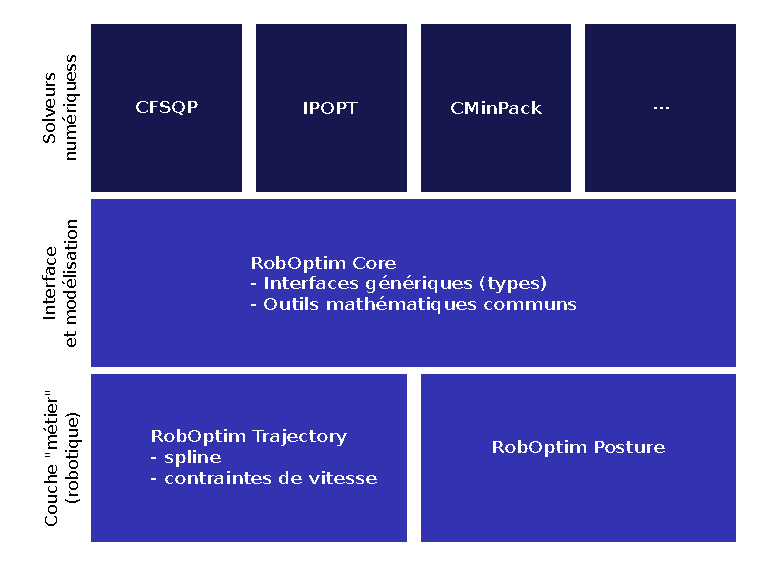
\includegraphics{src/chap1-roboptim/roboptim-architecture.pdf}
  \end{center}
  \caption{Architecture logicielle de RobOptim}
\end{figure}

\subsection{RobOptim core et ses plug-ins}

Le noyau de RobOptim fournit la modélisation mathématique des
fonctions, la classe définissant les problèmes d'optimisation ainsi
que les interfaces pour les solveurs. Le noyau, toutefois, ne contient
aucun algorithme de résolution. Ce paquet principal contient également
les outils mathématiques utiles pour résoudre les problèmes. Par
exemple, on peut augmenter le niveau de différenciabilité d'une
fonction via l'utilisation d'une méthode numérique se fondant sur la
méthode des différences finies. Cette méthode permet d'évalue la
dérivée d'une fonction en tirant des points aux alentours d'un point
de référence pour évaluer la courbure de la fonction aux alentours de
ce point. Plusieurs stratégies sont implémentées tirant deux ou cinq
points selon les cas. Cette fonctionnalité est implémentée via
l'utilisation du ``Design Pattern''\index{Design Pattern (motif de
  conception)} décorateur\index{Design Pattern (motif de
  conception)!Visiteur} tel que décrit dans le livre de
référence~\citep{design.pattern}. Ce motif de conception a la
particularité d'augmenter les capacités d'une classe sans en altérer
le comportement propre. Dans ce cas, cette classes paramétrée prend un
type de fonction en entrée, en hérite, tout en fournissant un niveau
de calcul supplémentaire des dérivées. D'autres outils permettent de
combiner des fonctions: les sommer, soustraire, multiplier entre elles
ou bien encore les combiner. Un autre décorateur fournit également un
cache afin d'éviter d'avoir à effectuer une nouvelle fois des calculs
lourds qui ont déjà été demandé précédemment.

Au delà de la définition des fonctions, le noyau fournit l'interface
pour les solveurs. Deux solutions sont alors possibles: soit se lier à
une ou des bibliothèques tierces fournissant des algorithmes de
résolution, soit utiliser le système de plug-in\index{plug-in}
permettant d'en charger à l'execution. L'objectif de ce système est de
pouvoir complètement déléguer au système la résolution d'un problème:
il y a un certain nombre de solveurs disponibles sur le système et
l'on pourrait ainsi, avoir une sélection automatique de l'algorithme
adéquat en fonction du type de problème en entrée. En pratique, ce
méchanisme permet simplement de pouvoir changer de solveur pendant
l'exécution du programme.


\subsection{Les solveurs}


Il est important d'insister sur le fait que ce travail n'a pas pour
but d'écrire un nouveau solveur ou bien de tenter d'apporter des
améliorations à une ou des approches existantes. La littérature du
domaine est foisonante et bénéficie d'un effort de recherche
important. Toutefois, l'objectif final de ce travail reste la
possibilité de pouvoir utiliser dans un même paradigme plusieurs
solveurs de types différents. Des plug-ins RobOptim ont été écrit pour
trois solveurs:
%
\begin{description}
\item[CMinPack\index{CMinPack}] solveur permettant de résoudre des problèmes de type
  moindre carrés linéaires,
\item[CFSQP\index{CFSQP}] solveur pour les problèmes non-linéaires, contraintes
  égalités et inégalités, calcul du gradient requis,
\item[IPOPT\index{IPOPT}] solveur pour les problèmes non-linéaires, contraintes
  égalités et inégalités, calcul du gradient et hessien
  requis\footnote{Une version alternative qui ne nécessite pas le
    calcul du hessien est également fournis par le paquet logiciel.}.
\end{description}

Ces solveurs sont disponibles sous la forme de plug-in pour RobOptim
core et peuvent être chargés dynamiquement dans n'importe quel
problème d'optimisation RobOptim.


\subsection{Optimisation de trajectoires avec RobOptim}

Un paradigme de programmation unifié permet également d'unifier les
outils de développement. En effet, le développement de bibliothèques
de fonctions de coût et de contraintes prend tout son sens une fois
que l'on a pu montrer que la même architecture est utilisable quelque
soit la structure du problème à résoudre. De ce constat, RobOptim
s'est enrichi d'une couche propre à la robotique, l'optimisation de
trajectoires.

Cette couche définit des trajectoires robotiques sous forme de
splines\index{spline}, c'est à dire de courbes
paramétrées\index{courbe paramétrée} par des points de
contrôle\index{point de contrôle}. Il est alors naturel de tenter de
vouloir altérer ces points de contrôle afin de rafiner le comportement
de la trajectoire: tenter de minimiser le temps nécessaire pour
réaliser le mouvement, ou l'énergie ou tout autre critère adéquat.

Cette bibliothèque fournit des bornes sur les vitesses du système à la
fois pour la vitesse de rotation et les vitesses linéaires. Le
problème d'optimisation de trajectoires est un problème semi-infini
dans la mesure où un souhait raisonnable est, par exemple, de borner
la vitesse du robot à tout moment de la trajectoire. Malheureusement,
la résolution de ce type de problèmes dans le cas général est
difficile et la technique la plus couramment utilisée reste une
discrétisation temporelle des contraintes. Ces stratégies présente
l'inconvénient d'augmenter très largement le nombre du contrainte du
problème. De plus, le pas de discrétisation est difficile à évaluer et
a un très fort impact sur la vitesse de résolution. Enfin, si on
ajoute la possibilité d'accélérer ou de décélérer la trajectoire au
problème, le solveur peut tenter de changer la paramétrisation
temporelle afin de placer toutes les contraintes au début du mouvement
et pouvoir, par exemple, passer au travers d'un obstacle. Un tel
comportement peut être éviter en attachant la contrainte non pas à un
moment temporel donné mais plutôt à un point de la trajectoire
indépendamment de sa paramétrisation temporelle. Il suffit pour cela
de se donner une échelle fixe, de 0 à 1, représentant respectivement
le début et la fin de la trajectoire, et permettant aux contraintes de
se déplacer avec la reparamétrisation de la trajectoire. La
discrétisation de contraintes utilisant ce type de représentation est
supporté par RobOptim et permet de simplifier la résolution de
problèmes d'optimisation de trajectoires.


\section{Scénaro d'utilisation: écriture d'une application robotique complexe}


Afin d'illustrer les propos des sections précédentes, nous allons
désormais nous attacher à résoudre un problème de robotique avec le
paradigme de RobOptim. L'exemple choisi est un problème de robotique
humanoïde. Une stratégie possible pour pouvoir générer une trajectoire
de marche est de tout d'abord générer un ensemble d'empreintes de pas
et ensuite de générer un mouvement tel que le robot place
successivement ses pieds dans les empreintes de pas générées tout en
conservant son équilibre. Si cette stratégie est adoptée, le problème
initial se ramène à trouver une pile de pas appropriée pour passer
d'un point $A$ à un point $B$. Ce dernier problème se ramène lui-même
à trouver le mouvement sans collision dans le plan d'une boîte en
rotation et translation. Une fois cette trajectoire trouvée, il suffit
de placer les pas le long de la trajectoire de la boîte pour obtenir
la pile de pas souhaitée.


Pour planifier le mouvement de la boîte, nous avons choisi d'utiliser
un algorithme aléatoire de type RRT -- Rapidly exploring Random Tree
--. Cet arbre va tenter d'échantillonner l'espace $\mathbb{R}^2 \times
SO(1)$ des translations et rotation en deux dimensions tout en validant
que les configurations tirées ne violent pas de contraintes ainsi que
le chemin amenant du n\oe ud le plus proche au nouveau n\oe ud
tiré. Malheureusement, cette méthode rend des trajectoires rarement
réalistes et qui ne sont pas toujours acceptables. Il est donc courant
d'utiliser une méthode probabiliste pour trouver un premier chemin
évitant les collisions qui est ensuite améliorée dans une deuxième
passe réalisée par un algorithme d'optimisation. C'est cette seconde
passe que nous avons choisi d'exprimer dans le paradigme de RobOptim.


\subsection{Définition de la trajectoire et fonction de coût}

\subsection{B-Splines et courbes paramétrées}

Comme indiqué dans la section précédente, les trajectoires sont
définies sous la forme d'une courbe paramétrée. Ce type de courbe
appelé B-spline\index{spline!B-spline} est définie comme une
combinaison linéaire d'une famille de fonctions de base. Les deux
définitions ci-dessous permettent de calculer analytiquement ces
courbes et sont tirées de~\citep{algo.3d}

\begin{mydef}\label{def:chap1_coxdeboor}
  Soit $n \in \mathbb{N}$, le nombre de points de contrôles. Soit $k
  \geq 1$, le degré des polynômes considérés. Soit $\Xi = (t_0, \dotsc,
  t_{n+k-1})$ un vecteur appelé, vecteur nodal avec $t_0 \geq \dotsc
  \geq t_{n+k-1}$. Les valeurs $t_i$ sont appelés noeuds. Les
  fonctions de base $N_{i,k}$ que nous allons définir, et donc les
  courbes B-splines que nous construirons ensuite, sont les
  polynomiales sur chaque intervalle $[t_i,t_{i+1}]$, pour $i =
  0,\dotsc,n-2$.

  La fonction $N_{i,k}$ est définie par récurrence\index{récurrence},
  comme suit:

  Pour $i = 0, \dotsc, n+k-2$, on pose:

  \begin{equation}
    N_{i,1}(t) = \left\{
  \begin{array}{l l}
    1 & \quad \text{si $t_i \leq t \leq t_{i+1}$ et $i = 0$ ou $t \neq t_i$} \\
    0 & \quad \text{sinon} \\
  \end{array} \right.
  \end{equation}

  Pour $r \geq 2$ et pour $i = 0, \dotsc, n + k - 1 - r$, on a la
  formule de récurrence:

  \begin{equation}
    N_{i,r}(t) = \frac{t - t_i}{t_{i+r-1}-t_i} N_{i,r-1}(t) +
    \frac{t_{i+r} - t}{t_{i+r} - t_{i+1}} N_{i+1,r-1}(t)
  \end{equation}

  La formule permettant de calculer les $N_{i,r}$ à partir des
  $N_{j,r-1}$ s'appelle la formule de Cox-de-Boor\index{Cox-de-Boor
    (formule de)}. Lorsque les dénominateurs de la formule s'annulent,
  on pose $\frac{0}{0} = 0$. C'est le cas lorsque plusieurs n\oe uds
  $t_i$ sont confondus.

\end{mydef}

\begin{mydef}\label{def:chap1_spline}
  Soit maintenant $P_0, \dotsc, P_{n-1}$ des points de contrôle. La
  courbe B-spline Q d'ordre $n$ et de degré $k - 1$ aillant $\Xi$ pour
  vecteur nodal et les $P_i$ pour points de contrôle s'exprime comme:

  \begin{equation}
    \left\{
    \begin{array}{ccc}
      Q : [t_{k-1},t_n] & \rightarrow & \mathbb{R}^3\\
      t & \mapsto & Q(t) = \sum_{i=0}^{n-1} P_i N_{i,k}(t)
    \end{array}
    \right.
  \end{equation}

  La courbe Q s'exprime donc comme une somme des fonctions $N_{i,k}$,
  pondérée par les points de contrôle.
\end{mydef}


Dans notre application, nous avons choisi d'utiliser des B-splines
uniforme de degré 3. Une B-spline est dîte uniforme lorsque les
intervalles temporels entre les points de contrôle définis par le
vecteur nodal $\Xi$ est constant entre chaque point de contrôle. Dans
notre cas, cette valeur sera dénotée $\lambda$ et fera parti des
variables d'optimisation. Les autres variables d'optimisation sont les
points de contrôle eux-mêmes, soit trois variables par point de
contrôle: $(x,y) \in \mathbb{R}^2$ la position du robot dans le plan
et $\theta \in S^1$ l'orientation du robot. Le vecteur de variables
d'optimisation ainsi constitué est illustra par
la~\autoref{tbl:param}.

\begin{table}[htbp]
  \begin{center}
\definecolor{LightGreen}{rgb}{0,.75,0}
\definecolor{DarkGreen}{rgb}{0,.25,0}
\begin{tabular}{|l|l l l|l|l l l|}
  \hline
  \textcolor{red}{$\lambda$}
  & \textcolor{LightGreen}{$x_0$}
  & \textcolor{LightGreen}{$y_0$}
  & \textcolor{LightGreen}{$\theta_0$}
  & \ldots
  & \textcolor{DarkGreen}{$x_n$}
  & \textcolor{DarkGreen}{$y_n$}
  & \textcolor{DarkGreen}{$\theta_n$} \\
  \hline
\end{tabular}
  \end{center}
  \caption{Variables d'optimisation du problème. \label{tbl:param}}
\end{table}

\subsubsection{Fonction de coût}


La paramétrisation choisit permet d'accélérer la courbe. En effet,
plus la valeur de $\lambda$ décroît plus la courbe est
accélérée. L'objectif est alors simplement de tenter de réaliser le
mouvement le plus vite possible. On réalise alors une optimisation
temps minimal\index{temps minimal} utilisant la fonction de coût
suivante:

\begin{eqnarray}
\text{Coût}(\mathbf{x}) & = & (1, 0, \dotsc, 0)^T \mathbf{x}
\end{eqnarray}

Dans les faits, le solveur va progressivement saturer les contraintes
en accélérant la courbe. En particulier jusqu'à ce que la contrainte
de vitesse détaille ci-dessous soit saturée. La~\autoref{fig:speed}
montre le processus de saturation d'une contrainte sur la vitesse dans
le cadre d'une spline unidimensionnelle.

\begin{figure}[htbp]
  \begin{center}
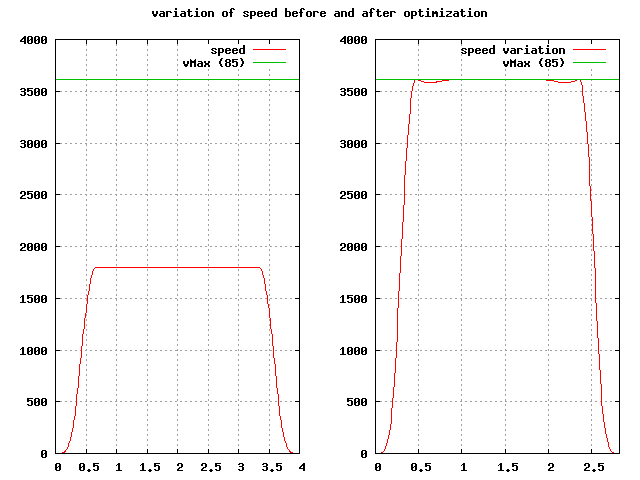
\includegraphics[width=\linewidth]{src/chap1-roboptim/time-optimization.png}
  \end{center}
  \caption{Saturation de la contrainte vitesse. \label{fig:speed}}
\end{figure}


\subsection{Contraintes}

\subsubsection{Contrainte sur la vitesse}

\index{Contrainte!de vitesse}
Le but de la contrainte sur les vitesses est double: s'assurer de la
correction de la trajectoire générée tout en privilégiant la marche en
avant par rapport à la marche sur le côté. Outre l'aspect
anthropomorphique, les robots humanoïdes ont un comportement dégradé
quand ils marchent ``en crabe''. L'espace accessible par les jambes
est réduit dans cette direction et la conception des semelles du robot
ont tendance à le faire glisser dans ce cas. Les contraintes sur les
vitesses sont dupliquées afin de s'appliquer à la fois au pied gauche
et au pied droit. La formulation de la contrainte pour tous les points
de la trajectoire $t$ et pour chaque pied est:

\begin{equation}
  \begin{split}
  \forall t, \forall \text{pied} \in \{\text{gauche}, \text{droite}\}, &\\
  \text{ContrainteVitesse}_{(t,\text{pied})}(\mathbf{x}) & =
  (\frac{v_{\text{pied}}^{x}}{v_{\text{max}}^{x}})^2 +
  (\frac{v_{\text{pied}}^{y}}{v_{\text{max}}^{y}})^2 - 1
  \end{split}
\end{equation}

$v_{\text{pied}}^{x}$ et $v_{\text{pied}}^{y}$ étant respectivement
les vitesses frontales et orthogonales du pied
considéré. $v_{\text{max}}^x$ et $v_{\text{max}}^y$ respectivement les
vitesses frontales et orthogonales maximum du robot. Plus le ratio
$\frac{v_{\text{max}}^x}{v_{\text{max}}^y}$ est élevé, plus le robot
privilégiera la marche en avant pendant l'optimisation au détriment de
la vitesse d'exécution du mouvement.

Cette contrainte impose à la vitesse des pieds de rester dans une
ellipse allongée vers l'avant. Cette contraine impose un mouvement
privilégiant la marche en avant et s'assure que le mouvement des pieds
est suffisamment lent pour pouvoir être jouée sur le robot. Afin
d'être certain que la contrainte est vérifiée en permanence, le temps
est discrétisé et on ajoute la contrainte pour tous les pas de temps.

\begin{figure}[htbp]
  \begin{center}
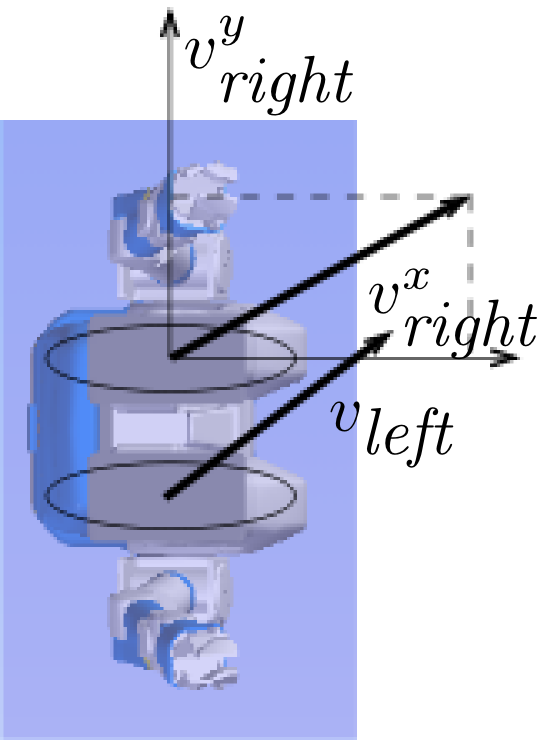
\includegraphics[width=5cm]{src/chap1-roboptim/speed-constraint-arrows.png}
  \end{center} \caption{Vitesses séparées du pied gauche et du pied
  droit. \label{fig:boxoptim}}
\end{figure}
\FloatBarrier


\subsubsection{Contrainte sur les obstacles}

\index{Contrainte!d'évitement des obstacles}
Les contraintes sur les obstacles se définissent naturellement: on
souhaite maintenir une distance minimale entre le robot et chaque
obstacle à tout moment. Comme avec la contrainte précédente, on
discrétise le temps afin de vérifier régulièrement la contrainte le
long de la trajectoire. La contrainte en tous points de la trajectoire
$t$ et pour tous les obstacles est la suivante:

\begin{eqnarray}
\forall t, \forall j, \text{Distance}(\mathcal{R}(t), \mathcal{O}_j) \geq d_{\min}
\end{eqnarray}

$\mathcal{R}$ représente ici la position du robot et $\mathcal{O}_j$
la position de l'obstacle $j$ de l'environnement. $d_{min}$ représente
une distance de sécurité déterminée empiriquement entre les obstacles
et le robot.


\subsection{Résolution et résultats expérimentaux}


La fonction de coût est une fonction linéaire mais les contraintes
sont non-linéaires. Il est nécessaire de définir des types RobOptim
pour ces fonctions, le type de problème associé:
$\text{Problème}_{\text{FonctionLinéaire}, \text{Fonction}_1}$. Le
gradient analytique a été déterminé pour toutes les fonctions afin
d'accélérer les calculs. Les calculs des fonctions et des gradients
associés sont détaillés dans FIXME. La~\autoref{fig:obstacle} montre
un exemple de chemin optimisé par le solveur CFSQP en simulation et
la~\autoref{fig:results} un exemple d'application sur le
robot. Le~\autoref{tbl:benchmarks} illustre les temps de calcul
rencontrés sur deux scénarios.

\begin{figure}[htbp]
  \begin{center}
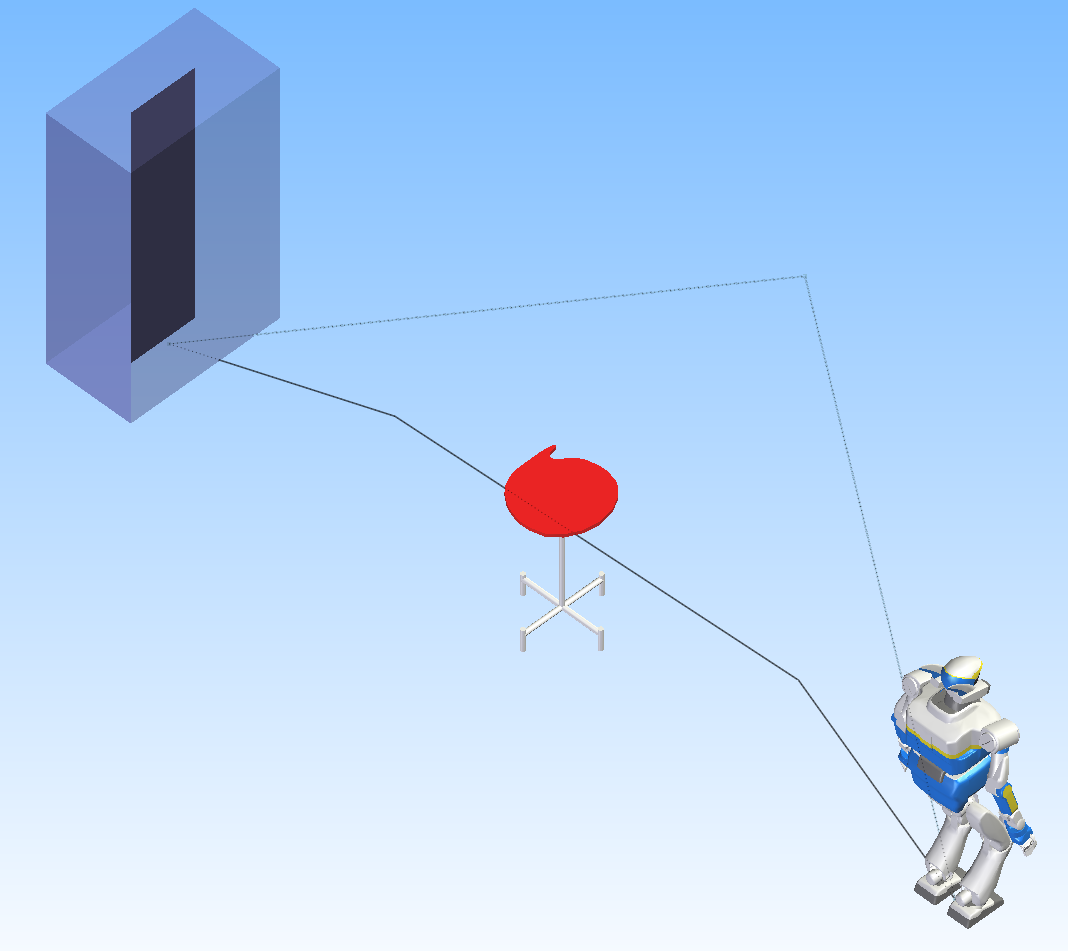
\includegraphics[width=.8\linewidth]{src/chap1-roboptim/straight-line-obstacle.png}
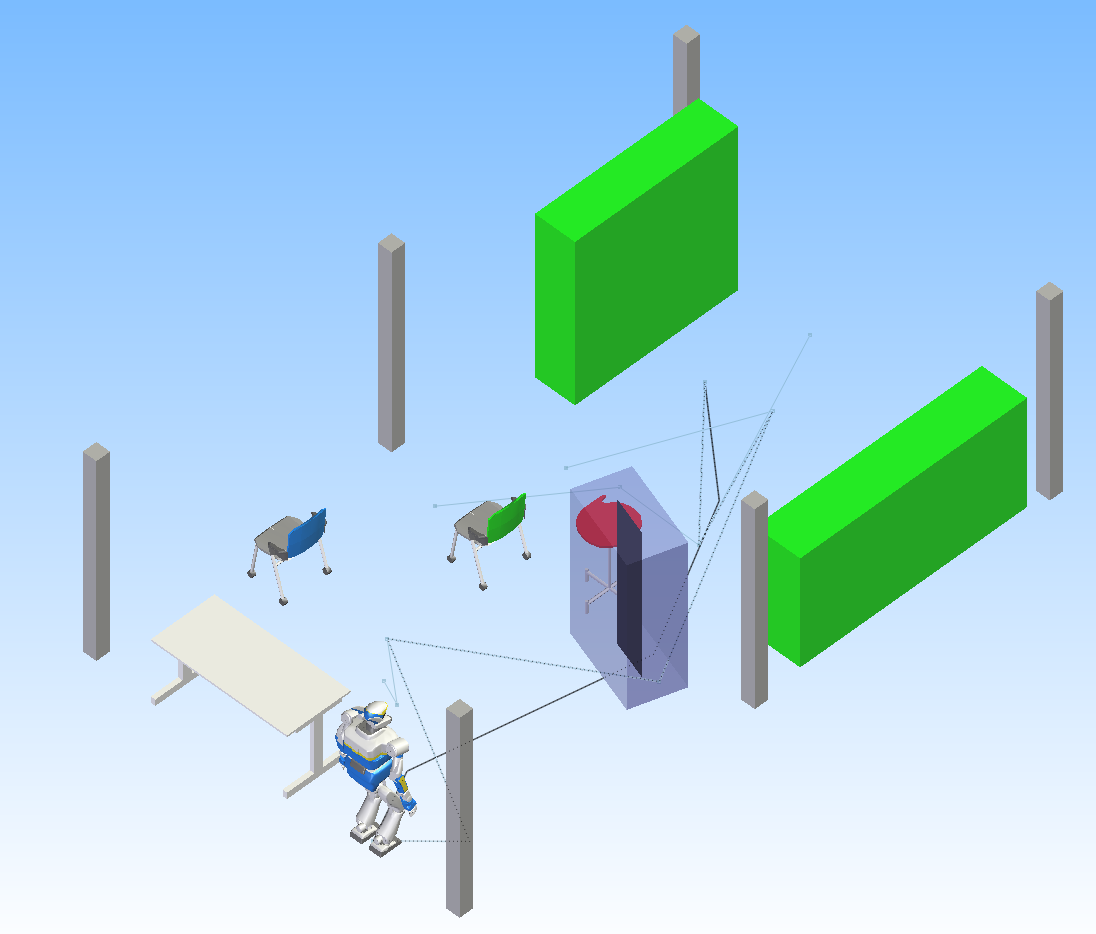
\includegraphics[width=.8\linewidth]{src/chap1-roboptim/optim-length.png}
  \end{center} \caption{Exemples d'optimisation d'une trajectoire en
  présence d'obstacles. \label{fig:obstacle}}
\end{figure}

\begin{figure}[htbp]
  \begin{center}
    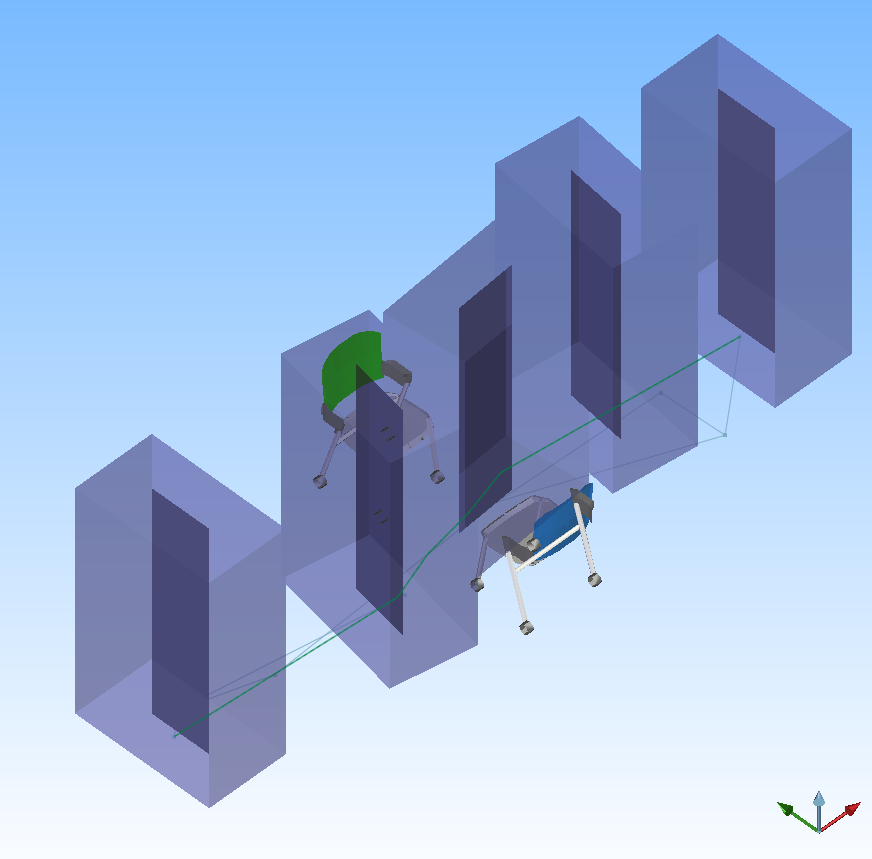
\includegraphics[width=\linewidth]{src/chap1-roboptim/two-chairs.png}
    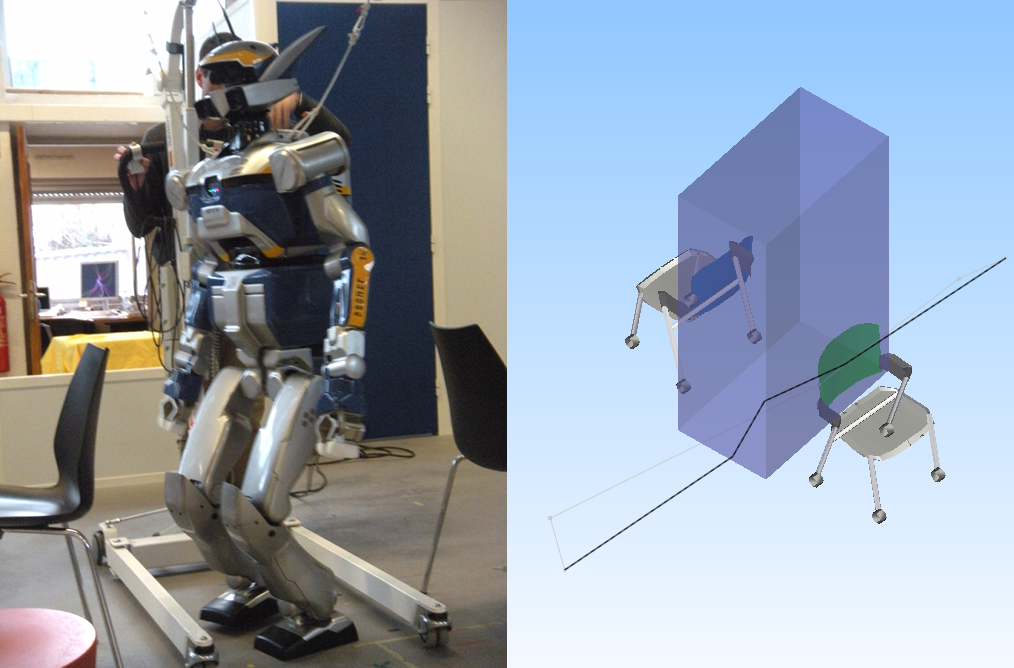
\includegraphics[width=\linewidth]{src/chap1-roboptim/hrp2-two-chairs.png}
  \end{center}
 \caption{Résultat expérimental sur le robot humanoïde
   HRP-2. \label{fig:results}}
\end{figure}

\begin{table}
  \begin{center}
    \begin{tabular}{|c|l l l|l|}
      \hline \bf Scenarii & Planification & Optimisation &
      \emph{Calcul complet}\\ \hline \bf Passage entre deux chaises &
      8.58s & 47.22s & \emph{2 min 05.55 s}\\ \hline \bf Salle
      réaliste avec de nombreux obstacles & 4.14 s & 1 min 9.35 s &
      \emph{4 min 5.11 s}\\ \hline
    \end{tabular}
  \end{center}
  \caption{Temps de calculs. Le temps de calcul complet comprends la
    planification, l'optimisation et la phase de génération de
    mouvement corps complet.\label{tbl:benchmarks}}
\end{table}


\section{Conclusion}

Ce chapitre a été dédié a la conception d'une modélisation orienté
objet pour la résolution de problèmes d'optimisation numériques ainsi
qu'à son implémentation, la suite logicielle RobOptim. Après avoir
observé les solveurs disponibles sur le marché, on peut facilement
s'apercevoir de l'écart considérable entre d'un côté la théorie
mathématique et son implémentation en pratique. En pratique, chaque
solveur vient avec son formalisme, ses interfaces et force ses
utilisateurs à apprendre une nouvelle formalisation pour chaque
nouveau solveur utilisé. De ce fait, réaliser des comparaisons est
mal-aisé, l'apprentissage inutilement difficile et les interfaces
souvent peu claires ou mal documentées. En fournissant un point
d'entrée pour plusieurs algorithmes, il n'y a qu'une interface et un
paradigme à expliquer ce qui présente un gain net vis-à-vis de
l'approche habituelle. De plus, de nombreux outils sont utiles en
optimisation tout en étant décorrélé de l'algorithme de résolution. Le
calcul des gradients par différence finies est un bon exemple. Dans
RobOptim, il a été intégré à la fois pour pouvoir éviter d'avoir à
calculer les gradients de manière analytique mais il peut également
servir à vérifier le gradient analytique. Du point de vue logiciel,
l'accent a été mis sur la création d'un ensemble de bibliothèques
logicielles simples à utiliser et assurant la correction du problème
posé. Cette correction passe par l'utilisation d'un système de typage
fort permettant de détecter à la compilation les problèmes qui peuvent
se poser. En effet, RobOptim interdit, à la compilation, la
construction d'un problème invalide: si certains gradients sont
manquants ou bien si certains types de fonction sont incorrects, la
compilation du fichier échouera car les contraintes de typage ne
seront pas respectées. Malgré ce système de typage imposant des règles
strictes, une grande flexibilité a été gardée dans le choix de
l'algorithme qui peut s'effectuer à l'exécution. Le système de plug-in
de RobOptim permettant de charger les algorithmes dynamiquement
pendant l'exécution du programme. La suite logicielle a été validée
sur un exemple réel de robotique qu'est l'optimisation de trajectoire
de marche pour un robot humanoïde.

\chapter{Suivi de trajectoire}
\label{chap:suivi}

\epigraph{Text text text text text text text text text text text text
  text text text text text text text text text text text text text
  text text text text text text text text text text text text text
  text text text text text text text text text text text text text
  text text text text}{Some Author}
\clearpage

\lettrine[lines=2, lraise=0.1, nindent=0em, slope=-.5em]%
{C}{e} chapitre est dédié au problème de la génération et de
l'exécution asservie de trajetoires pour un robot humanoïde. Les
robots humanoïdes sont des robots aillant une forme anthropomorphique:
une tête, deux bras, deux jambes et un torse. La locomotion est donc
bipède et les robots humanoïdes ont la possibilité d'effectuer des
tâches dextres. De ces choix résultent un système hautement dimensioné
pour lequel il est difficile de générer des trajectoires et dont le
contrôle est délicat, l'équilibre d'un système bipède étant précaire
par nature. Au long de ce chapitre, nous verrons comment modéliser ce
système, comment représenter et calculer des mouvements pour ce
dernier afin qu'il puisse se mouvoir et réaliser différentes
tâches. Serons ensuite étudiée les différentes approches de la
littérature ainsi que leurs forces et leurs faiblesses. La troisième
section portera sur l'apport de cette thèse au problème de l'exécution
de trajectoire via la proposition d'une architecture de contrôle pour
les robots humanoïdes asservie capteur. Les résultats expérimentaux
seront ensuite détaillés pour illustrer une tâche dans laquelle le
système proposé se révèle utile. Enfin, les prospectives montreront
quelles sont les possibilités d'améliorations de l'approche proposée
et quels futurs travaux restent à réaliser.

\section{Génération de mouvements pour les robots humanoïdes}
\subsection{Structure robotique}

Un robot est un système composé par des actionneurs -- moteurs --, des
capteurs et des unités de calcul logique -- ordinateurs -- travaillant
de concert pour constituer une entité cohérente pouvant impacter le
monde réel afin de réaliser l'objectif qui lui a été confié. En ce qui
concerne la génération de l'exécution de mouvements, deux éléments
sont primordiaux: d'une part les capacités motrices du système,
modélisés sous la forme d'un arbre cinématique et d'autre part sa
forme dans le monde représentée par la forme géométrique des
différentes partie du système. La forme géométrique d'un robot variant
généralement sous l'action de ses actionneurs, elle est donc
conditionée par l'état de l'arbre cinématique.

\begin{mydef}
  Un arbre cinématique est un ensemble de joints formant un arbre.
  Soit $\mathcal{A}$ un arbre cinématique, on a:

  \begin{equation}
    \mathcal{A} = \emptyset \cup \{ (\mathcal{J}_0, \mathcal{C}_0),
    \dotsc, (\mathcal{J}_n, \mathcal{C}_n) \}
  \end{equation}

  Un arbre est donc soit l'ensemble vide soit une liste de joints
  associé à un sous-arbre. Cette définition permet de construire
  récursivement un arbre cinématique.

  A cet arbre de joints correspond une liste de joints, les joints
  sont habituellement référencés par leur ordre dans cette liste sous
  la notation $\mathcal{J}_n$ où $n$ est la position du joint dans la
  liste.
\end{mydef}

\begin{mydef}
  Le joint $\mathcal{J}_n$ modélise le mouvement du repère $n+1$ par
  rapport au repère $n$ selon un certain nombre de paramètres appelés
  degrés de liberté. Chaque joint définit implicitement son repère
  attaché. Le repère attaché à $\mathcal{J}_0$ est habituellement
  appelé repère ``monde'' et est noté $\mathcal{W}$.

  Un joint peut donc se modéliser comme une fonction:

  \begin{equation}
    \left\{
    \begin{array}{cccc}
      \mathcal{J}_n : & \mathbb{R}^m & \rightarrow & SE(3)\\
      & \mathbf{q} & \mapsto & \mathcal{J}_n(t)
    \end{array}
    \right.
  \end{equation}

  Dans l'équation le joint $\mathcal{J}_n$ possède $m$ degrés de
  liberté permettant de déterminer la transformation relative entre le
  repère $n$ et $n + 1$ qui est un élément du groupe spécial euclidien
  de dimension 3. Ces fonctions permettent donc d'exprimer des
  contraintes sur les mouvements des corps du robot au niveau des
  articulations actionées.
\end{mydef}

Plusieurs types de joints sont habituellement utilisés en robotique,
mais nous n'allons ici en détailler que deux:
\begin{description}
\item[Joint libre -- ou joint flottant --] Ce joint comporte six degrés de libertés, soit le
  nombre de paramètres nécessaire et suffisant pour spécifier une pose
  dans $SE(3)$. Autrement dit, ce joint n'impose aucune contrainte
  particulière sur le mouvement et correspond donc à la fonction
  identité, à la représentation de la pose près.
\item[Joint rotation] Ce joint comporte un seul degré de liberté. Dans
  ce cas, la position du prochain corps du robot est défini par la
  valeur de ce degré de liberté, interprété comme une rotation d'un
  angle équivalent autour d'un axe. A chaque joint rotation est donc
  soit associé un axe de rotation, soit un axe standard est choisi:
  par exemple, toutes les rotations seront réalisées autour de l'axe
  X.
\end{description}


Une fois cette structure construite, un souhaite naturel est de
souhaiter pouvoir exprimer son état. C'est l'objectif du vecteur de
configuration.

\begin{mydef}
  Soit $\mathbf{q}$ le vecteur de configuration de l'arbre cinématique
  $\mathcal{C}$. Soit $\mathcal{J}_0, \dotsc, \mathcal{J}_n$
  l'ensemble des joints de $\mathcal{C}$. Le vecteur de configuration
  a pour dimension: $\sum_{i=0}^n \#\mathcal{J}_i$, la somme des arités
  des joints interprétés comme fonctions, c'est à dire la somme du
  nombre de degrés de liberté de tous les joints.


  Les valeurs du vecteur de configuration sont alors les valeurs des
  degrés de liberté des joints concaténés les uns aux autres selon un
  parcours de l'arbre donné. En général, le parcours main gauche de
  l'arbre est utilisé.
\end{mydef}

\begin{figure}[htbp!]
  \begin{center}
  \begin{tikzpicture}
    \Tree [ .{$\mathcal{J}_0$ (6)} [ .{$\mathcal{J}_1$ (1)} {$\mathcal{J}_2$ (2)} {$\mathcal{J}_3$ (1)} ] {$\mathcal{J}_4$ (1)} ]
  \end{tikzpicture}

  \begin{tabular}{|ccc|c|cc|c|c|}
    \hline
    $\mathcal{J}_0$ (1) & \ldots & $\mathcal{J}_0$ (6)
    & $\mathcal{J}_1$ (1) & $\mathcal{J}_2$ (1) & $\mathcal{J}_2$ (2) & $\mathcal{J}_3$ (1) & $\mathcal{J}_4$ (1)\\
    \hline
  \end{tabular}
  \end{center}

  \caption{Un exemple de chaîne cinématique et son vecteur de
    configuration correspondant. Les nombres entre parenthèses
    indiquent le nombre de degrés de liberté dans l'arbre ou le numéro
    du degré de liberté dans le joint pour le vecteur de
    configuration.}
\end{figure}

On notera que l'arbre cinématique d'un robot humanoïde est souvent
composé d'un joint libre à la racine suivi de joints rotation pour le
reste de l'arbre. À partir de maintenant, cette forme sera
systématiquement utilisée ce qui nous permettra de diviser le vecteur
de configuration en deux parties: d'un côté la position du robot dans
le plan, définie par une sous-partie des degrés de liberté du joint
libre à la racine, le repère de ce joint définissant de ce fait le
repère monde $\mathcal{W}$ et d'autre part les degrés de liberté
internes correspondant à une réalité méchanique. On aura donc:

\begin{equation} \label{eq:chap2_configuration}
  \begin{aligned}
    \mathbf{x} &= [x, y, r_z]\\
    \mathbf{q} &= (\mathbf{x}, [z, r_x, r_y, \mathbf{q}_{\text{int}}])
    \in \mathcal{C} = \text{SE}(2) \times \mathcal{C}_{\text{int}}
  \end{aligned}
\end{equation}

Les six paramètres du joint racine sont: $[x, y, z, r_x, r_y, r_z]$ et
définissent une position dans l'espace 3d. Toutefois, dans la mesure
où la position du robot est contrainte par la physique, c'est à dire
que l'on peut raisonnablement supposer un contact planaire entre les
pieds du robot et le sol, on peut se contenter de considérer la
position du robot en deux dimensions dans le plan. Pour cette raison,
on peut considérer: $\mathbf{x} = [x, y, r_z] \in \text{SE}(2)$ pour
déterminer la position du robot dans l'espace. $\mathcal{C}$
représente alors l'espace des configurations et
$\mathcal{C}_{\text{int}}$ est l'espace des configurations
correspondant aux degrés de liberté internes uniquement. Ce découpage
peut sembler arbitaire au premier abord mais prend son sens quand on
considère quels degrés de liberté peuvent dériver suite à des erreurs
de modélisation ou d'exécution: la position du robot dans le plan peut
s'avérer fausse et doit être estimée et corrrigée constamment alors
que les degrés de liberté $[z, r_x, r_y]$ ne peuvent pas subir de
dérives durant le mouvement. Le problème de la correction des erreurs
est détaillé plus loin dans ce chapitre et le problème de la
localisation d'un robot humanoïde est abordée dans le chapitre
suivant.


Une fois cette chaîne cinématique définie, on peut y attacher les
informations concernant les corps du robot, leur réalité physique:
forme et information inertielles en particulier. La forme est stoquée
sous la forme d'une soupe de polygones réalisant une approximation de
la forme originale du corps du robot. Quant aux informations
inertielles, elles consistent en le poids du corps, la position de son
centre de masse et sa matrice d'inertie.


\subsection{Cinématique directe et inverse}

\subsubsection{Cinématique directe}

A partir de la structure définie dans la section précédente, la
première opération que l'on souhaite pouvoir réaliser est pouvoir
déterminer la position des corps du robot en fonction de la
configuration de ce dernier. Cette opération, appelée calcul de la géométrie directe, consiste en la fonction suivante:
\begin{equation}
  \text{GéométrieDirecte}_{\mathcal{C}}(q) = \{
  \transformation{\mathcal{W}}{\mathcal{J}_0}, \dotsc,
  \transformation{\mathcal{W}}{\mathcal{J}_n} \}
\end{equation}

La notation $\transformation{\mathcal{A}}{\mathcal{B}}$ représente la
transformation qui donne la position du repère $\mathcal{B}$ relative
au repère $\mathcal{A}$. L'intéret de cette représentation est de pouvoir assembler les transformations facilement, en effet, on a:

\begin{equation}
  \transformation{\mathcal{A}}{\mathcal{C}} = \transformation{\mathcal{A}}{\mathcal{B}} \transformation{\mathcal{B}}{\mathcal{C}}
\end{equation}
%FIXME: pas de sens sans definir le ops, ici multiplication matricielle


La géométrie directe donne donc la position de tous les corps dans le
repère monde. Dans la section précédente, on a défini un joint comme
la position du repère attaché au joint suivant par rapport à la
position du joint actuel.

\begin{mydef}\label{def:chap2-geomdirect}
Soit $\mathcal{J}_n$ un joint de l'arbre cinématique et $\Delta =
\{\mathcal{J}_0, \dotsc, \mathcal{J}_n\}$ le chemin dans l'arbre de la
racine au noeud $\mathcal{J}_n$. Soit $\mathbf{q}_i$ les degrés de
liberté du joint $\mathcal{J}_i$. La position du joint $\mathcal{J}_n$
dans le repère monde est:
\begin{equation}
  \transformation{\mathcal{W}}{\mathcal{F}_i} = \prod_{j \in \Delta} \mathcal{J}_j (\mathbf{q}_j)
\end{equation}
\end{mydef}


\subsubsection{Cinématique inverse}

La Définition~\autoref{def:chap2-geomdirect} permet de construire la
position de tous les corps du robot dans le repère monde attaché au
joint racine de la structure. Cependant, lors de la conception d'un
problème robotique, il est courant de vouloir, par exemple,
positionner un effecteur du robot -- un préhenseur par exemple -- à un
endroit particulier de l'espace Euclidien. Dans ce cas, le problème
inverse doit être résolu: trouver une configuration telle qu'un corps
particulier du robot atteigne une position donnée. Ce problème est
appelé géométrie inverse.


Une difficulté de ce problème est que l'on doit inverser une équation
dont le nombre de variables correspond au nombre de degrés de liberté
du robot et dépend évidemment de sa structure. Si l'on souhaite
positionner un corps à un endroit précis en rotation et translation,
six variables sont nécessaires. De ce fait, selon le nombre de degrés
de liberté du système et la position à atteindre, 0, 1 ou une infinité
de solutions peuvent exister. La résolution analytique n'étant pas
toujours possible, les outils numériques ont montré leur capacité à
résoudre efficacement ce problème. Une technique de résolution
possible sera détaillée dans la section~FIXME.

FIXME: vitesse des corps

\subsection{Mouvements dynamiques d'un corps dans l'espace}

La géométrie et cinématique permettent de calculer la vitesse de corps
dans l'espace indépendamment de leur réalité physique. Cependant, ce
n'est pas suffisant pour pouvoir générer un mouvement complexe: le
poids des corps du robot, leurs propriétés inertielles ainsi les
forces exercées s'appliquant au robot doivent être prises en compte
pour pouvoir donner un mouvement qui n'est pas seulement viable dans
un monde sans physique, mais également dans le monde réel où les lois
de la physique s'appliquent.

Pour se faire, nous allons commencer par rappeler les notions de
mécanique nécessaire à la génération de mouvements et les différents
modèles simplifiés utilisés en robotique humanoïde. Tout l'enjeu de la
robotique humanoïde se joue ici: d'un côté on ne peut ignorer la
physique pour générer un mouvement de marche mais de l'autre le coût
important de la résolution des modèles de la physique classique
Newtonienne empêche l'écriture de contrôleurs suffisamment rapides
pour pouvoir fonctionner en temps réel sur un robot. Il y a ici un
compromis à trouver qui fait toute la richesse de la robotique
humanoïde: quelles simplifications adopter? quels calculs peuvent être
réalisés à l'avance, une fois pour toute, et quels calculs doivent
être fait en ligne? Nous allons tout d'abord nous attacher à rappeler
les lois de la mécanique classique avant de nous intéresser aux
différentes simplifications qui permettent de rendre le problème
tractable.


\subsubsection{Quelques éléments de mécanique}
\paragraph{Lois fondamentales de la mécanique}

\begin{mydef}(Relation fondamentale de la dynamique)\\
  Tout point de masse $m$ de position $M$ soumis à un ensemble de
  forces dont la somme est $\vect{F}$ est mû par un mouvement
  d'accélération $\gamma$ donnée par la relation suivante:
  \begin{equation}\label{eq:newton}
    \vect{F} = m \ddot{\vect{x}}
  \end{equation}
\end{mydef}

\begin{mydef}(Principe d'action-réaction)\\
  Soient $P_1$ et $P_2$ deux points de masses respectives $m_1$ et
  $m_2$. Si $\vect{F}_{1/2}$ est la force exercée par $P_1$ sur $P_2$ et
  $\vect{F}_{2/1}$ la force exercée par $P_2$ sur $P_1$, alors:
  \begin{equation}\label{eq:reaction}
    \vect{F}_{1/2} = -\vect{F}_{2/1}
  \end{equation}
\end{mydef}

\begin{mydef}(Principe de colinéarité)\\
  Soient $P_1$ et $P_2$ deux
  points de masses respectives $m_1$ et $m_2$. La force $\vect{F}_{1/2}$
  exercée par $P_1$ sur $P_2$ est colinéaire au vecteur $\vec{P_1P_2}$
\end{mydef}

\paragraph{Systèmes de points}

\begin{mydef}(Moment d'un vecteur en un point)\\
  Soit $\vect{V}$ un vecteur de point d'application $M$. Le moment en
  un point $O$ de $\vect{V}$ est défini par le produit vectoriel
  suivant:
  $$
  \moment{\vect{V}}{O} = \vec{OM} \crossprod \vect{V}
  $$
\end{mydef}

Dans toute cette section, $(P_i)_{i=1,...,n}$ est un système de points de masses respectives $m_i$,
de positions respectives $M_i$, de vitesses respectives $\vi$ et d'accélérations respectives $\gammai$.

Pour chaque point $P_i$, on peut écrire la relation fondamentale de la
dynamique~(\ref{eq:newton}) en distinguant les forces internes
$\vect{F}_{j/i}$ appliquées par les autres points du système et les
forces externes $\vect{F}^{ext}_{i}$
issues de causes externes au système:
$$
\sum_{j=1, j\not=i}^n \vect{F}_{j/i} + \vect{F}^{ext}_{i} = m_i
\gammai
$$
On peut également écrive le moment de chaque membre de cette égalité
en un point $O$:
$$
\sum_{j=1, j\not=i}^n \vec{OM_i}\crossprod \vect{F}_{j/i} +
\vec{OM_i}\crossprod\vect{F}^{ext}_{i} = m_i \vec{OM_i}\crossprod \gammai
$$
En sommant les deux égalités précédentes pour tous les points du
système, les termes relatifs aux forces internes s'annulent par les
principes d'action-réaction et de colinéarité. En effet, si on
considère deux points $P_i$ et $P_j$ du systèmes les forces relatives
à ces deux points vérifient:
$$
\vect{F}_{i/j} + \vect{F}_{j/i} = 0
$$
et
\begin{eqnarray*}
\vec{OM_i}\crossprod \vect{F}_{j/i} + \vec{OM_j}\crossprod
\vect{F}_{i/j}&=&
\vec{OM_i}\crossprod \vect{F}_{j/i} - \vec{OM_j}\crossprod
\vect{F}_{j/i} \\
&=&
\vec{M_{j}M_{i}} \crossprod \vect{F}_{j/i} \\
&=& 0
\end{eqnarray*}
La dernière égalité découle du principe de colinéarité.
Il en résulte les égalités suivantes:
\begin{eqnarray}
\label{eq:1}
\sum_{i=1}^n \vect{F}^{ext}_{i} &=& \sum_{i=1}^n m_i \gammai \\
\label{eq:2}
\sum_{i=1}^n \vec{OM_i}\crossprod\vect{F}^{ext}_{i}
&=& \sum_{i=1}^n m_i \vec{OM_i}\crossprod \gammai
\end{eqnarray}

\begin{mydef}(Centre de masse)\\
  Soit $G$ le centre de masse et $M$ la
  masse totale du système de
  points:
  $$
  G = \frac{1}{M}\sum_{i=1}^{n} m_i M_i
  $$
\end{mydef}

En dérivant deux fois cette égalité, on en déduit l'accélération du
centre de masse du système:
$$
\gammaG = \frac{1}{M}\sum_{i=1}^{n} m_i \gammai
$$
Cette expression injectée dans (\ref{eq:1}) nous donne la propriété
suivante bien connue: la somme des forces appliquées à un système est
égale à la masse du système que multiplie l'accélération de son centre
de masse.
$$
\sum_{i=1}^n \vect{F}^{ext}_{i} = M \gammaG \\
$$
Cette propriété découle de la relation fondamentale de la dynamique et
du principe d'action-réaction.


\paragraph{Torseurs}

\begin{mydef} (Torseur)\\
  Un torseur est un champ de vecteurs $\vect{M}$ qui vérifie la propriété
  suivante: il existe un vecteur $\vect{R}$ tel que pour tout couple de
  points $O$ et $P$ la relation suivante soit satisfaite:
  $$
  \vect{M}_O = \vect{M}_P + \vec{OP} \crossprod \vect{R}
  $$
  $\vect{R}$ est unique. Il est appelé la {\em résultante} du torseur
  noté:
  $$
  \left\{\vect{M}_O|\vect{R}\right\}_{O}
  $$
\end{mydef}

\begin{myexample} (Le torseur des vitesses d'un solide)\\
  Le champ de vecteurs des vitesses d'un solide est un torseur dont la
  résultante est le vecteur vitesse de rotation généralement noté
  $\vec{\omega}$.
\end{myexample}

\begin{myexample} (Le champ des moments des forces extérieures sur un système)\\
  Si l'on considère le système de points $P_i$ soumis à des forces
  extérieures $\vect{F}_i^{ext}$, on définit le moment de ces forces en
  un point $O$ par:
  $$
  \moment{}{O} = \sum_{i=1}^{n} \vec{OM_i}\crossprod \vect{F}_i^{ext}
  $$
  On vérifie alors aisément que ce champ de moment est un torseur dont
  la résultante est la somme des $\vect{F}_i^{ext}$. En
  effet,
  \begin{eqnarray*}
    \moment{}{O} &=& \sum_{i=1}^{n} \vec{OM_i}\crossprod \vect{F}_i^{ext}
    =\sum_{i=1}^{n} (\vec{OP}+\vec{PM_i})\crossprod \vect{F}_i^{ext} \\
    &=& \sum_{i=1}^{n} \vec{OP}\crossprod \vect{F}_i^{ext} +
    \vec{PM_i}\crossprod \vect{F}_i^{ext} \\
    &=& \moment{}{P} + \vec{OP} \crossprod \sum_{i=1}^{n} \vect{F}_i^{ext}
  \end{eqnarray*}
\end{myexample}


\paragraph{Torseur cinétique}

Le torseur cinétique d'un système de points est le champ, noté $\vec{\sigma}$, des
moments de quantités de mouvement du système:
$$
\vec{\sigma}_{O} = \sum_{i=1}^n \vec{OM_i} \crossprod m_i \vi
$$
La résultante du torseur cinétique est la quantité de mouvement du
système:
$$
\vect{P} = \sum_{i=1}^n m_i \vi
$$
Si $O$ est un point fixe, on peut dériver la relation suivante
pour obtenir:
\begin{eqnarray*}
  \dot{\vec{\sigma}}_O &=& \sum_{i=1}^n \vi \crossprod m_i \vi + \vec{OM_i}
  \crossprod m_i \gammai \\
  &=& \sum_{i=1}^n \vec{OM_i} \crossprod m_i \gammai
\end{eqnarray*}
Cette dernière égalité nous permet d'énoncer la propriété suivante:
\begin{property}
  la dérivée du moment cinétique d'un système de points par rapport à un
  point fixe est égale au
  moment des forces extérieures par rapport à ce point sur le système:
  \begin{equation}\label{eq:newton3}
    \dot{\vec{\sigma}}_0 = \moment{\vect{F}^{ext}}{O}
  \end{equation}

  La dérivée de la résultante cinétique est égale à la résultante des
  forces extérieures:
  \begin{equation}\label{eq:newton2}
    \dot{\vect{P}} = \sum_{i=1}^n \vect{F}_i^{ext}
  \end{equation}

\end{property}

\textbf{Remarque:} il est aisément vérifiable que la propriété du
moment cinétique est valide également au centre de masse même si
celui-ci n'est pas fixe:
$$
\dot{\vec{\sigma}}_G = \moment{\vect{F}^{ext}}{G}
$$

\paragraph{Cas des solides}

Un solide est un ensemble d'atomes considérés comme des masses
ponctuelles. Les efforts que ces points exercent les uns sur les
autres respectent les principes d'action-réaction et de colinéarité.
Un approximation courante consiste à considérer les solides comme des milieux
continus. Cela a pour conséquence de remplacer les sommes par des
intégrales dans les résultats précédents.

\begin{mydef} (Torseur cinétique)\\

Dans le cas d'un solide, la résultante cinétique ou quantité de
mouvement devient:
$$
P = \int_S \vect{v}_M dm(M)
$$
où $dm(M)$ est la mesure de densité massique et $\vect{v}$ le champ
des vitesses qui rappelons le est un torseur:
$$
\vect{v}_M = \vG + \vec{MG}\crossprod \vec{\omega}
$$
Il en résulte que:
\begin{eqnarray*}
P &=& \int_S (\vG + \vec{MG}\crossprod \vec{\omega}) dm(M) \\
&=& M\vG + \int_S (\vec{MG}) dm(M)\crossprod \vec{\omega} \\
&=& M\vG
\end{eqnarray*}
par définition du centre de masse.
\end{mydef}

Le moment cinétique au centre de masse s'écrit:
\begin{eqnarray*}
\vec{\sigma}_G &=& \int_S \vec{GM}\crossprod \vect{v}_M dm(M)\\
&=& \int_S \vec{GM}\crossprod (\vG+\vec{\omega}\crossprod\vec{GM})dm(M)\\
&=& \int_S \vec{GM}dm(M)\crossprod\vG +
\int_S \vec{GM}\crossprod(\vec{\omega}\crossprod\vec{GM})dm(M)\\
&=& \int_S \vec{GM}\crossprod(\vec{\omega}\crossprod\vec{GM})dm(M)\\
\end{eqnarray*}
par définition du centre de masse.

\textbf{Remarque:} Il est intéressant de remarquer les deux points
suivants:
\begin{enumerate}
  \item L'opérateur $\hat{J}$ qui à $\vec{\omega}$ associe $\vec{\sigma}_G$
    est linéaire. Sa matrice dans toute base orthonormée est
    symétrique positive définie.
  \item  $\vec{\omega}$ et $\vec{\sigma}_G$ ne sont en général pas colinéaires.
\end{enumerate}


\subsubsection{ZMP}

\begin{figure}
  \centerline {
    \input{zmp.pdftex_t}
  }
  \caption{L'équilibre statique du pied implique que le torseur des
    efforts extérieurs: l'effet de la gravité, la réaction du sol et
    l'action du robot sur le pied s'annule.}
  \label{fig:zmp}
\end{figure}

Nous considérons maintenant un robot humanoïde muni de deux pieds
plats en phase de simple contact. La définition et l'analyse du ZMP
reposent sur la condition de stabilité du pied du robot en contact avec
le sol supposé horizontal.

Considérons donc le pied en contact avec le sol. Les actions
extérieures appliquées sur ce pied sont (Figure~\ref{fig:zmp}):
\begin{enumerate}
  \item l'action du robot privé de son pied sur la cheville,
    représentée par le torseur:
    $$
    \left\{\vect{M}^{robot}_A | \vect{R}^{robot} \right\}_{A}
    $$
    où $A$ est le centre de l'articulation de la cheville.
  \item l'action de la gravité sur le pied représentée par le torseur
    $$
    \left\{\vect{0} | m \vect{g} \right\}_{G}
    $$
    où $G$ est le centre de masse du pied, $\vect{g}$ le vecteur
    d'accélération due à la gravité et $m$ la masse du pied.
  \item l'action du sol sur le pied représentée par le torseur
    $$
    \left\{\vect{M}^{ground}_O | \vect{R}^{ground} \right\}_{G}
    $$
    où $O$ est l'origine du repère supposée appartenir au plan du sol.
\end{enumerate}
L'hypothèse de stabilité du pied sur le sol s'exprime donc par 6
équations qui lient les résultantes et moments ci-dessus. En supposant
connus le poids et le centre de masse du pied, l'action du robot sur
le pied, on peut en déduire l'action du sol sur le pied puis vérifier
que cette action est possible étant donné que les efforts de contact
du sol sur le pied ont une composante verticale positive.
Ecrivons ces équations:
\begin{eqnarray*}
  \vect{R}^{robot}+ m \vect{g}+ \vect{R}^{ground} &=& 0 \\
  \vect{M}^{robot}_A + \vec{OA}\crossprod\vect{R}^{robot}
  +\vec{OG}\crossprod m\vect{g} + \vect{M}^{ground}_O &=& 0
\end{eqnarray*}
Ainsi l'action du sol sur le pied est donnée par:
\begin{eqnarray*}
  \vect{R}^{ground} &=& -\vect{R}^{robot} - m \vect{g} \\
  \vect{M}^{ground}_O &=& -\vect{M}^{robot}_A - \vec{OA}\crossprod\vect{R}^{robot}
  - \vec{OG}\crossprod m\vect{g}
\end{eqnarray*}

\paragraph{Définition du ZMP}

Le ZMP est le point du sol en lequel les composantes horizontales du
moment du sol sur le pied sont nulles. Nous le notons $Z$. Exprimons
le moment des actions du sol sur le pied en $Z=(Z_x,Z_y,0)$:
\begin{eqnarray*}
\vect{M}_Z^{ground} &=& \vect{M}_O^{ground} + \vec{ZO}\crossprod
\vect{R}^{ground} \\
&=& \left(\begin{array}{c} M^{ground}_{O\,x} \\ M^{ground}_{O\,y} \\ M^{ground}_{O\,z}
\end{array}\right)
+
\left(\begin{array}{c} -Z_x \\ -Z_y \\ 0
\end{array}\right)
\crossprod
\left(\begin{array}{c} R^{ground}_x \\ R^{ground}_y \\ R^{ground}_z
\end{array}\right) \\
&=&
\left(\begin{array}{c}
M^{ground}_{O\,x} - Z_y R^{ground}_z\\
M^{ground}_{O\,y} + Z_x R^{ground}_z \\
M^{ground}_{O\,z} + Z_y R^{ground}_x - Z_x R^{ground}_y
\end{array}\right)
\end{eqnarray*}
L'annulation des deux premières composantes donne lieu à deux
équations dont les inconnues sont $Z_x$ et $Z_y$. Ce système
d'équations est régulier si et seulement si la composante $R^{ground}_z$
est non-nulle, hypothèse raisonnable dans la phase de simple support
du robot. Les coordonnées du ZMP sont dans ce cas:
$$
ZMP =
\left(\begin{array}{c}
-\frac{M^{ground}_{O\,y}}{R^{ground}_z} \\
\frac{M^{ground}_{O\,x}}{R^{ground}_z} \\
0
\end{array}\right)
$$
\subsection{Pourquoi le ZMP doit-il rester dans le polygone support ?}

Pour répondre à cette question, nous modélisons l'action du sol sur le
pied par un champ de forces défini dans la partie $S$ du plan
correspondant à la zone de contact du pied. Nous notons
$$
\vect{F}(x,y) = \left(\begin{array}{c}
f_x(x,y) \\ f_y(x,y) \\ f_z(x,y)
\end{array}\right)
$$
la force du sol sur le pied au point de coordonnées $(x,y,0)$. Le moment des actions du sol sur le pied au
ZMP s'exprime donc de la façon suivante:
\begin{eqnarray*}
\vect{M}^{ground}_{ZMP} = \int_S \vec{Z_{mp}M} \crossprod \vect{f}(x,y) dS(M)
\end{eqnarray*}
où $dS(M)$ est une mesure surfacique.
Les composantes horizontales de ce moment s'écrivent:
\begin{eqnarray}\label{eq:3}
  \int_S (y-Z_y)f_z(x,y) dx dy &=& 0 \\
  \label{eq:4}
  \int_S (Z_x-x)f_z(x,y) dx dy &=& 0 \\
\end{eqnarray}
Supposons que le ZMP soit en dehors de l'enveloppe convexe de la
surface d'appui (non-nécessairement polygonale). Alors, il existe une
droite qui sépare le ZMP de la surface d'appui. Au prix d'un
changement de repère, on peut supposer que cette droite est l'axe
$O\vec{y}$ du repère, que $Z_x < 0$ et que tous les points de la surface
d'appui ont des abscisses positives. Le terme $(Z_x-x)$ de l'intégrale
de l'équation~(\ref{eq:4}) est donc uniformément négatif sur $S$ et
donc (\ref{eq:4}) ne peut être satisfaite que si $f_z$ est
uniformément nulle, condition exclue par nos hypothèses.

Ainsi, une condition nécessaire de stabilité du pied sur le sol est
que le ZMP soit dans l'enveloppe convexe de la surface d'appui.


\paragraph{Le ZMP comme critère d'équilibre}

La position du ZMP peut également être calculée à partir de la dérivée du moment cinétique et de la résultante cinétique du robot.
Exprimons les équations de la dynamique~(\ref{eq:newton3}) et (\ref{eq:newton2}) au centre de masse du robot:
\begin{eqnarray*}
m\dot{\vect{v}}_G &=& \vect{R}^{ground} + m \vect{g} \\
\dot{\sigma}_G &=& \vect{M}_G^{ground}
\end{eqnarray*}
Exprimons maintenant le moment des forces du sol sur le robot en un point $Z=(x_Z, y_Z, 0)$ du sol:
\begin{eqnarray*}
\vect{M}_Z^{ground} &=& \vect{M}_G^{ground} + \vec{ZG} \crossprod (\vect{R}^{ground}) \\
&=& \dot{\sigma}_G + m \vec{ZG} \crossprod (\dot{\vect{v}}_G - m\vect{g})
\end{eqnarray*}
En notant $\sigma_G = ({\sigma}_x, {\sigma}_y, {\sigma}_z)$ et $(x_G, y_G, z_G)$ la position du centre de masse, l'équation précédente s'écrit:
\begin{eqnarray*}
\vect{M}_Z^{ground} &=& \left(\begin{array}{lll}
\dot{\sigma}_x\ +\ m\ (y_G - y_Z)\ (\ddot{z}_G + g)\ -\ m\ z_G\ \ddot{y}_G \\
\dot{\sigma}_y\ +\ m\ z_G\ \ddot{x}_G\ -\ m\ (x_G-x_Z)\ (\ddot{z}_G + g) \\
\dot{\sigma}_z\ +\ m\ (x_G - x_Z)\ \ddot{y}_G\ -\ m\ (y_G-y_Z)\ \ddot{x}_G
\end{array}\right)
\end{eqnarray*}
Pour exprimer les coordonnées du ZMP, il suffit de résoudre le système d'équations obtenu en annulant les composantes $x$ et $y$ de $\vect{M}_Z^{ground}$.
Nous obtenons alors:
\begin{eqnarray*}
x_{ZMP} &=& x_G - \frac{\dot{\sigma}_y\ +\ m\ z_G\ \ddot{x}_G}{m\ (\ddot{z}_G + g)} \\
y_{ZMP} &=& y_G + \frac{\dot{\sigma}_x\ -\ m\ z_G\ \ddot{y}_G}{m\ (\ddot{z}_G + g)}
\end{eqnarray*}

\paragraph{Mouvement de marche dynamique}

\begin{figure}
  \centerline{
    \input{dynamics.pdftex_t}
  }
  \caption{Efforts internes et externes exercés sur le robot.}
  \label{fig:dynamics}
\end{figure}

Dans cette section, nous établissons les équations de mouvement
dynamique d'un robot en phase de simple appui sur le sol, composé d'un
corps ${\cal B}$, d'une jambe ${\cal L}$, d'un tibia ${\cal S}$ et
d'un pied ${\cal F}$ et représenté sur la figure~\ref{fig:dynamics}.
Pour simplifier, nous supposons que ${\cal L}$ et ${\cal S}$ ont une masse
nulle. Nous notons ${\cal R}=(O,\vec{x},\vec{y},\vec{z})$ un repère
fixe de l'environnement.

Les différents efforts en présence sont les suivants:
\begin{itemize}
  \item $\vect{R}^{\cal B}$ la résultante du corps sur la jambe,
  \item $\vect{M}^{\cal B}_C$ le moment  appliqué par le
    corps sur la jambe en $C$,
  \item $\vect{R}^{\cal L}$ la résultante de la jambe sur le tibia,
  \item $\vect{M}^{\cal L}_B$ le moment  appliqué par la
    jambe sur le tibia en $B$,
  \item $\vect{R}^{\cal S}$ la résultante du tibia sur le pied,
  \item $\vect{M}^{\cal S}_A$ le moment  appliqué par le
    tibia sur le pied en $A$,
  \item $\vect{R}^{ground}$ la résultante du sol sur le pied,
  \item $\vect{M}^{ground}_O$ le moment appliqué par le sol sur le pied en $O$.
\end{itemize}

\subparagraph{Efforts sur la jambe et sur le tibia.}
En isolant successivement les corps ${\cal L}$ et ${\cal S}$ et en
écrivant les équations de la dynamiques pour ces corps, nous obtenons
les relations suivantes:
\begin{eqnarray}
  \label{eq:resultante-L}
  \vect{R}^{\cal B} - \vect{R}^{\cal L} &=& 0 \\
  \label{eq:resultante-S}
  \vect{R}^{\cal L} - \vect{R}^{\cal S} &=& 0 \\
  \label{eq:moment-L}
  \vect{M}^{\cal B}_C + \vec{BC}\crossprod \vect{R}^{\cal B} -
  \vect{M}^{\cal L}_B &=& 0 \\
  \label{eq:moment-S}
  \vect{M}^{\cal L}_B + \vec{AB}\crossprod \vect{R}^{\cal L} -
  \vect{M}^{\cal S}_A &=& 0
\end{eqnarray}

\subparagraph{Efforts sur le corps du robot.}
Les efforts qui s'appliquent sur le corps du robot sont la gravité et
les efforts de la jambe. Ces efforts donnent lieu aux deux équations
suivantes:
\begin{eqnarray}\label{eq:resultante-B}
m \vec{\gamma}_G &=& m\vect{g} - \vect{R}^{\cal B} \\
\label{eq:moment-B}
\frac{d\vec{\sigma}_G}{dt} &=& -\vec{GC}\crossprod \vect{R}^{\cal B} - \vect{M}^{\cal B}_C
\end{eqnarray}

Les équations~(\ref{eq:resultante-L}) et ~(\ref{eq:resultante-S})
représentent les résultantes des efforts exercés sur ${\cal L}$ et
${\cal S}$ respectivement. Elles permettent de conclure à l'égalité
des résultantes suivantes que nous notons $\vect{R}$:
$$
\vect{R}^{\cal B} = \vect{R}^{\cal L} = \vect{R}^{\cal S} = \vect{R}
$$
Les équations~(\ref{eq:moment-L}) et
(\ref{eq:moment-S}) représentent les moments en $B$ et $A$ des efforts
sur les corps ${\cal L}$ et ${\cal S}$ respectivement.

En notant $\theta_{\cal B}$,$\theta_{\cal L}$,$\theta_{\cal S}$ et
$\theta_{\cal F}$ respectivement l'orientation du corps par rapport à
l'axe $\vec{z}$, les angles relatifs de ${\cal L}$ par rapport à ${\cal B}$, de
${\cal S}$ par rapport à ${\cal L}$ de ${\cal F}$ par rapport à ${\cal
  S}$, et $l_{\cal B}$, $l_{\cal L}$, $l_{\cal S}$ les distance entre
$G$ et $C$, entre $B$ et $C$ et entre $A$ et $B$, nous avons les égalités suivantes:
$$
\vec{BC} =
\left(\begin{array}{c}
-l_{\cal L} \sin(\theta_{\cal B}+\theta_{\cal L}) \\
0\\
l_{\cal L} \cos(\theta_{\cal B}+\theta_{\cal L})
\end{array}\right)
\ \ \ \
\vec{AB} =
\left(\begin{array}{c}
-l_{\cal S} \sin(\theta_{\cal B}+\theta_{\cal L}+\theta_{\cal S}) \\
0\\
l_{\cal S} \cos(\theta_{\cal B}+\theta_{\cal L}+\theta_{\cal S})
\end{array}\right)
$$
\subparagraph{Position de $G$ et moment cinétique de ${\cal B}$.}
Les coordonnées de $G$ sont données par les relations suivantes:
\begin{eqnarray}
  \label{eq:xG}
  x_G &=& x_A -l_{\cal S} \sin(\theta_{\cal B}+\theta_{\cal
    L}+\theta_{\cal S}) -l_{\cal L} \sin(\theta_{\cal B}+\theta_{\cal
    L}) -l_{\cal B} \sin(\theta_{\cal B}) \\
  \label{eq:zG}
  z_G &=& z_A + l_{\cal S} \cos(\theta_{\cal B}+\theta_{\cal
    L}+\theta_{\cal S}) + l_{\cal L} \cos(\theta_{\cal B}+\theta_{\cal
    L}) + l_{\cal B} \cos(\theta_{\cal B})
\end{eqnarray}
A partir de maintenant, nous notons $\Theta = (\theta_{\cal B},
\theta_{\cal L}, \theta_{\cal S})$ un paramétrage de la configuration
du robot. Le moment cinétique du corps ${\cal B}$ s'écrit:
\begin{equation}\label{eq:sigma-G}
\vec{\sigma}_G = \hat{J}(\Theta) \vec{\omega}_{\cal B}
\end{equation}
où $\hat{J}(\Theta)$ est l'opérateur d'inertie de ${\cal B}$ dans
la configuration $\Theta$ et $\vec{\omega}_{\cal B} = \dot{\theta}_{\cal B}\vec{y}$ est le vecteur rotation du corps ${\cal B}$. La matrice de $\hat{J}(\theta_{\cal B})$
dans la base $(\vec{x},\vec{y},\vec{z})$ a pour expression:
$$
\left(\begin{array}{ccc}
\cos\theta_{\cal B} & 0 & -\sin\theta_{\cal B} \\
0 & 1 & 0 \\
\sin\theta_{\cal B} & 0 & \cos\theta_{\cal B}
\end{array}\right)
J_0
\left(\begin{array}{ccc}
\cos\theta_{\cal B} & 0 & \sin\theta_{\cal B} \\
0 & 1 & 0 \\
-\sin\theta_{\cal B} & 0 & \cos\theta_{\cal B}
\end{array}\right)
$$
où $J_0$ la matrice de $\hat{J}(0)$ dans la base $(\vec{x},\vec{y},\vec{z})$.

\subparagraph{Accélération du centre de masse.}
En dérivant~(\ref{eq:xG}) et (\ref{eq:zG}), on obtient une expression
de la forme:
\begin{eqnarray}
\label{eq:vG}
\vect{v}_G &=& M(\Theta) \dot{\Theta}
\end{eqnarray}
où
$$
M(\Theta) =
\left(\begin{array}{ccc}
z_A-z_G & z_A-z_C & z_A-z_B \\
0 & 0 & 0 \\
x_G-x_A & x_C-x_A & x_B-x_A
\end{array}\right)
$$
est une matrice qui dépend de la configuration du robot.
En dérivant~(\ref{eq:vG}) on obtient:
\begin{eqnarray}
\label{eq:gammaG}
\vec{\gamma}_G = M(\Theta)\ddot{\Theta} + \dot{M}(\Theta,\dot{\Theta})\dot{\Theta}
\end{eqnarray}
avec
{\tiny
$$
\begin{array}{l}
\dot{M}(\Theta,\dot{\Theta})=\\
\left(\begin{array}{ccc}
(x_A-x_G)\dot{\theta}_{\cal B}+(x_A-x_C)\dot{\theta}_{\cal
  L}+(x_A-x_B)\dot{\theta}_{\cal S} &
(x_A-x_C)(\dot{\theta}_{\cal B}+\dot{\theta}_{\cal L}) +
(x_A-x_B)(\dot{\theta}_{\cal S}) &
(x_A-x_B)(\dot{\theta}_{\cal B}+\dot{\theta}_{\cal
  L}+\dot{\theta}_{\cal S}) \\
0 & 0 & 0 \\
(z_A-z_G)\dot{\theta}_{\cal B}+(z_A-z_C)\dot{\theta}_{\cal
  L}+(z_A-z_B)\dot{\theta}_{\cal S} &
(z_A-z_C)(\dot{\theta}_{\cal B}+\dot{\theta}_{\cal L}) +
(z_A-z_B)(\dot{\theta}_{\cal S}) &
(z_A-z_B)(\dot{\theta}_{\cal B}+\dot{\theta}_{\cal
  L}+\dot{\theta}_{\cal S}) \\
\end{array}\right)
\end{array}
$$
}
D'après~(\ref{eq:resultante-B}), nous pouvons écrire:
\begin{eqnarray}\label{eq:R-1}
\vect{R} &=& m(\vect{g} -\vec{\gamma}_G) \\
\label{eq:R-2}
&=& m(\vect{g} - M(\Theta)\ddot{\Theta} - \dot{M}(\Theta,\dot{\Theta})\dot{\Theta})
\end{eqnarray}
En dérivant~(\ref{eq:sigma-G}), nous obtenons une expression de la
forme:
$$
\frac{d\vec{\sigma}_G}{dt} = \hat{J}(\Theta) \frac{d\vec{\omega}_{\cal
    B}}{dt} + \dot{\hat{J}}(\Theta,\dot{\Theta})\vec{\omega}_{\cal B}
$$
Grâce à~(\ref{eq:moment-B}), nous pouvons écrire la relation
suivante:
\begin{eqnarray}\label{eq:moment-C-1}
\vect{M}^{\cal B}_C &=& -\vec{GC}\crossprod \vect{R} -
\frac{d\vec{\sigma}_G}{dt} \\
\label{eq:moment-C-2}
&=& -\vec{GC}\crossprod \vect{R} -
\hat{J}(\Theta) \ddot{\theta}_{\cal B} \vec{z} -
\dot{\hat{J}}(\Theta,\dot{\Theta})\dot{\theta}_{\cal B} \vec{z}
\end{eqnarray}
En rassemblant les équations~(\ref{eq:R-2}) et (\ref{eq:moment-C-2})
et en utilisant les relations~(\ref{eq:moment-L}) et
(\ref{eq:moment-S}), nous arrivons au système suivant:
\begin{eqnarray}
\vect{R}&=& m(\vect{g} - M(\Theta)\ddot{\Theta} - \dot{M}(\Theta,\dot{\Theta})\dot{\Theta})\\
\vect{M}^{\cal B}_C&=& -\vec{GC}\crossprod \vect{R} -
\hat{J}(\Theta) \ddot{\theta}_{\cal B} \vec{z} -
\dot{\hat{J}}(\Theta,\dot{\Theta})\dot{\theta}_{\cal B} \vec{z}\\
\vect{M}^{\cal L}_B &=& \vect{M}^{\cal B}_C + \vec{BC}\crossprod \vect{R}  \\
\vect{M}^{\cal S}_A &=&\vect{M}^{\cal L}_B + \vec{AB}\crossprod \vect{R}
\end{eqnarray}

\subparagraph{Conclusion.} Etant donnée une trajectoire du système sous
la forme de l'évolution de $\Theta$ au cours du temps, les quatre
équations précédentes permettent de calculer
\begin{itemize}
  \item la réaction du tibia sur le pied $\vect{R}$,
  \item le moment $\vect{M}^{\cal B}_C$ appliqué sur la jambe par le moteur de
    l'articulation de la hanche,
  \item le moment $\vect{M}^{\cal L}_B$ appliqué sur le tibia par le
    moteur de l'articulation du genou,
    \item le moment $\vect{M}^{\cal S}_A$ appliqué sur le pied par le
      moteur de l'articulation de la cheville.
\end{itemize}
Les efforts du tibia sur le pied permettent ensuite de calculer la
position du ZMP et de vérifier que le mouvement est admissible.


\subsection{Génération d'une trajectoire de marche}

La section précédente a construit incrémentalement, à partir des lois
fondamentales de la dynamique, les relations nécessaires pour pouvoir
générer une trajectoire de marche pour un robot humanoïde. Il s'agit
désormais de choisir une stratégie de résolution qui ne soit non
seulement correcte, mais qui puisse être mise en place sur le robot
pour générer une trajectoire de marche stable.

\paragraph{Énoncé du problème}

La tâche à résoudre peut être énoncée ainsi: le robot doit aller du
point $A$ au point $B$ de façon à préserver son équilibre. La
stratégie la plus utilisée consiste en les étapes suivantes:
\begin{enumerate}
\item Planifier une série de points d'appuis, c'est à dire d'emprunte
  de pas reliant les deux points. Les techniques classiques de
  planification de mouvement tel que la programmation dynamique -- A*
  -- ou bien encore les algorithmes probabilistes type RRT peuvent
  être utilisés dans ce cadre. En sortie, nous avons donc une suite
  d'empreintes de pas pour les deux pieds du robot annoté d'un moment
  de début et d'un moment de fin. Les moments où les deux pieds du
  robot sont au sol sont appelés phase de double support et les
  moments où un seul pied est au sol les phase de simple support.
\item Le ZMP est alors utilisé comme critère de stabilité, on définit
  alors une trajectoire de ZMP telle qu'à tout moment le ZMP est dans
  l'enveloppe convexe des points de contacts. Une heuristique simple
  consiste à partir de la projection du centre de masse au sol au
  temps initial -- le ZMP et le centre de masse sont confondus à
  l'arrêt --, puis de passer le ZMP sous la cheville du pied gauche,
  réaliser un pas avec le pied droit, passer le ZMP sous la cheville
  du pied droit, réaliser un pas avec le pied gauche, etc. Il en
  ressort une trajectoire de référence pour le ZMP définie par une
  ligne brisée.
\item À partir de la trajectoire du ZMP, une trajectoire du centre de
  masse du robot doit être calculée. La section suivante détaillera
  ensuite comment suivre cette trajectoire du centre de masse pendant
  la marche.
\end{enumerate}

Le problème reste alors la troisisème étape: comment passer d'une
trajectoire de ZMP à une trajectoire de centre de masse tout en
préservant les contraintes temps réel qui sont inhérantes au contrôle
d'un système robotique.

\paragraph{De la réalité physique à un modèle calculatoire tractable}

Tout d'abord, rappelons la formule du ZMP:

\begin{equation}
\left(
\begin{array}{cc}
x_{\text{ZMP}}\\
y_{\text{ZMP}}
\end{array}
\right) = \left(
\begin{array}{cc}
x_G - \frac{\dot{\sigma}_y\ +\ m\ z_G\ \ddot{x}_G}{m\ (\ddot{z}_G + g)}\\
y_G + \frac{\dot{\sigma}_x\ -\ m\ z_G\ \ddot{y}_G}{m\ (\ddot{z}_G + g)}
\end{array}
\right)
\end{equation}

$x_G$, $y_G$, $z_G$ étant la position du centre de masse dans
l'espace, $\sigma$ le moment d'inertie du centre de masse, $m$ la
masse totale du robot et $g$ la constante de gravité. L'objectif ici
est de déduire $x_{G}$ à partir du $x_{ZMP}$ choisi. La résolution
d'une telle équation est malheureusement difficile car il n'existe pas
de solution analytique et les solutions numériques sont lentes et
nécessitent l'évaluation de plusieurs grandeurs dont le calcul du
moment d'inertie autour du centre de masse.

Cependant, cette équation peut devenir linéaire au prix des hypothèses suivantes:
\begin{itemize}
\item Moment d'inertie du centre de masse négligeable: $\dot{\sigma}_x = \dot{\sigma}_y = 0$
\item Hauteur du centre de masse constante: $z_G$ constant, $\ddot{z_G} = 0$
\end{itemize}

Ces hypothèses nous permettent d'obtenir les relations linéaires suivantes:
\begin{eqnarray*}
x_{\text{ZMP}} &=& x_G - \frac{z_G}{g} \ddot{x}_G\\
y_{\text{ZMP}} &=& y_G - \frac{z_G}{g} \ddot{y}_G
\end{eqnarray*}

Ce modèle dît du ``Pendule Inverse Linéarisé'' pose le problème sous
la forme d'une équation différentielle non-homogène du second
ordre. La résolution explicite d'une telle équation est possible et
peut s'exprimer sous la forme suivante:

\begin{equation}
  \mathbf{x}(t) = \cosh(\sqrt{\frac{g}{z_G}}.t) . \mathbf{V} + \sinh(\sqrt{\frac{g}{z_G}}.t) . \mathbf{W} + \mathbf{r}(t)
\end{equation}

$\mathbf{V}$ et $\mathbf{W}$ étant des constantes déterminées par les
conditions aux limites du système, à savoir que le centre de masse
atteigne la position fixée au début et à la fin avec une vitesse
nulle. $\textbf{r}(t)$ est un polynôme d'ordre 3, tout comme la
trajectoire du ZMP et dont les coefficients sont entièrement
déterminés par elle. Les valeurs de $\mathbf{V}$ et $\mathbf{W}$ sont
déterminées par les conditions aux limites du système:

\begin{equation}
  \left(
  \begin{array}{c}
    \mathbf{x}_x(0)\\
    \mathbf{x}_y(0)
  \end{array}
  \right) = \left(
  \begin{array}{c}
    \mathbf{V}_x + \mathbf{r}_x(0)\\
    \mathbf{V}_y + \mathbf{r}_y(0)
  \end{array}
  \right)
\end{equation}

\begin{equation}
  \left(
  \begin{array}{c}
    \dot{x}(0)\\
    \dot{y}(0)
  \end{array}
  \right) = \left(
  \begin{array}{c}
    \frac{g}{z_G} . \mathbf{W}_x + \dot{\mathbf{r}}_x(0)\\
    \frac{g}{z_G} . \mathbf{W}_y + \dot{\mathbf{r}}_y(0)
  \end{array}
  \right)
\end{equation}

Ces quatre variables nous permettent de pouvoir déterminer la position
et vitesse initiale du centre de masse. On a alors:

\begin{equation}
  \left(
  \begin{array}{c}
    \mathbf{V}_x\\
    \mathbf{V}_y
  \end{array}
  \right) = \left(
  \begin{array}{c}
    \mathbf{x}_x(0) - \mathbf{r}_x(0)\\
    \mathbf{x}_y(0) - \mathbf{r}_y(0)\\
  \end{array}
  \right)
\end{equation}

\begin{equation}
  \left(
  \begin{array}{c}
    \mathbf{W}_x\\
    \mathbf{W}_y
  \end{array}
  \right) = \left(
  \begin{array}{c}
    \frac{z_G}{g}(\dot{\mathbf{x}}_x(0) - \dot{\mathbf{r}}_x(0))\\
    \frac{z_G}{g}(\dot{\mathbf{x}}_y(0) - \dot{\mathbf{r}}_y(0))
  \end{array}
  \right)
\end{equation}

Cependant, nous n'avons pas de variable libre supplémentaire qui nous
permettrait de contraindre la position et vitesse finale ($t=T$) de la
trajectoire du centre de masse. Une stratégie pour contourner le
problème peut être alors de remarquer qu'un changement de
$\dot{\mathbf{x}}(0)$ fait varier $\mathbf{x}(T)$ de façon
monotone. Il est alors possible de réaliser une recherche par
dichotomie sur les valeurs de $\dot{\mathbf{x}}(0)$ afin de
contraindre la position finale du centre de masse. Dans la mesure où
l'on peut également adapter la longueur du pas $T$, il est possible de
choisir $T$ telle que les vitesses initiales et finales du centre de
masse peuvent être négligées et la trajectoire du centre de masse
considérée $\mathcal{C}^2$ sur la totalité de la trajectoire de
marche.


Cette stratégie de calcul a pour avantage d'être simple à comprendre
et à implémenter mais également peu coûteuse en terme de temps de
calcul. Elle a été développée par Nicolas Perrin dans~FIXME. Les
limites de cette approche se situent dans les nombreuses hypothèses
limitantes du modèle simplifié ainsi que par la recherche dichotomique
des paramètres adaptés pour assurer la continuité de la trajectoire de
centre de masse.


\subsection{Exécution d'une trajectoire}


La section précédente a montré comment générer, à partir d'une
séquence d'empreintes de pas, une trajectoire de centre de masse qui
assure la stabilité du robot. Une fois cette trajectoire associée aux
trajectoires des pieds, on obtient une représentation une
représentation d'une trajectoire de marche. Cette représentation est
avantageuse car elle ne fixe pas directement la position des corps du
robot, il est alors encore possible de déplacer le haut du corps pour,
par exemple, aller saisir un objet. Ce type de tâche étant typiquement
définie comme un asservissement sur la donnée d'un capteur, il est
nécessaire de pouvoir découpler ce qui relève de la planification et
donc d'un processus lent et ce qui relève de l'asservissement capteur,
c'est à dire d'un comportement réactif. On peut alors se demander,
comment passer d'une série de trajectoires à une commande pouvant être
envoyée aux actionneurs du système.


Ce problème peut se résoudre en tant que problème d'optimisation:
l'objectif serait de minimiser la vitesse des actionneurs tout en
ajoutant des contraintes pour suivre les trajectoire de référence. On
pourrait imaginer avoir trois contraines pour la trajectoire du centre
de masse et des deux pieds. Il est alors possible d'ajouter encore une
contrainte, pour atteindre un objet à saisir avec la main, par
exemple.


C'est à ce moment qu'une différenciation s'opère entre d'un côté les
stratégies d'optimisation numériques classiques et les stratégies
d'optimisation adaptées à la robotique de l'autre. Les problèmes que
la robotique traite possèdent deux caractistiques qui les rend
spécifique:
\begin{enumerate}
\item Ils n'admettent pas toujours une solution: il est possible
  l'objet soit trop loin pour pouvoir être atteint.
\item Les contraintes du problème ont une importance variable: suivre
  les trajectoires de référence sur les pieds et le centre de masse
  est critique car ces contraintes permettent d'assurer la stabilité
  du robot. Échouer la saisie d'un objet est comparativement beaucoup
  moins important car il sera toujours possible de retenter la saisie
  sans que cela mette le système dans une situation critique.
\end{enumerate}

Enfin, le suivi de trajectoire et la génération de la commande doit
être réalisée à une fréquence fixe. Le solveur doit donc pouvoir
réaliser une itération durant un tour de la boucle temps réel ce qui
impose des limitations très strictes sur la complexité des calculs
pouvant être réalisé. Face à ces particularités, la stratégie de
résolution adoptée ici est celle de la ``pîle de tâches''.


\subsubsection{Tâche et pile de tâches}

\paragraph{Tâche}

L'objectif d'un contrôleur est de pouvoir calculer la commande à
envoyer aux actionneurs qui va réaliser un certain nombre d'objectifs
assignés au robot. Habituellement, il est mal aisé d'exprimer ses
objectifs directement dans l'espace des commandes du système. À la
place, nous pouvons exprimer ces objectifs sous forme de tâche. Chaque
tâche vît dans un espace qui lui est propre et adapté à la contrainte
que l'on souhaite exprimer. Par exemple, dans le cas d'un
asservissement visuel, l'espace de la tâche sera l'espace image
2d. Une tâche d'asservissement visuel sera alors de réaliser un
mouvement tel qu'un ensemble de points de l'image puisse atteindre une
position prédéfinie.

\begin{mydef}
Une tâche est une fonction calculant l'erreur entre l'état courant
d'une amer noté $s$ et un état de référence pré-défini de cet amer
noté $s*$:

\begin{equation}
  \mathbf{e} = \mathbf{s} - \mathbf{s}^{*}
\end{equation}

L'objectif est donc de réaliser la tâche, c'est à dire de ramener
l'erreur calculée par la tâche à zéro. L'erreur d'une tâche peut être
de dimension supérieure à 1, dans ce cas l'objectif est de ramener
toutes les composantes du vecteur d'erreur à $0$. La définition de
l'opérateur de comparaison entre les deux états est dépendant de
l'espace de la tâche.
\end{mydef}

\paragraph{Jacobien}

La résolution d'une tâche passe par l'utilisation du jacobien de la
tâche. Ce dernier est noté:

\begin{equation}
  \mathbf{J}_i = \frac{\partial \mathbf{e}_i}{\partial \mathbf{q}}
\end{equation}

Il lie l'espace des vitesses de la tâche à l'espace des vitesses
articulaires du robot via la relation:

\begin{equation}
  \dot{\mathbf{e}}_i = \mathbf{J}_i \dot{\mathbf{q}}
\end{equation}


\paragraph{Pile de tâches}

On peut calculer la vitesse articulaire du robot en inversant la
relation précédente:

\begin{equation}
  \dot{\mathbf{q}} = \mathbf{J}_1^{+} \dot{\mathbf{e}}_1^{*} + \mathbf{P}_1 \mathbf{z}
\end{equation}

$\mathbf{J}_1^{+}$ est la pseudo-inverse de $\mathbf{J}_1$ ou inverse
des moindre carrés de $\mathbf{J}_1$. $\dot{\mathbf{e}}_1$, la
consigne, est le mouvement souhaité dans l'espace de la
tâche. $\mathbf{P}_1$ est le projecteur vectoriel sur le noyau du
jacobien $\mathbf{J}_1$ et $\mathbf{z}$ un vecteur quelconque. Le
projecteur est défini par:

\begin{equation}
  \mathbf{P}_1 = \mathbf{I} - \mathbf{J}_1^{+} \mathbf{J}_1
\end{equation}

Ce projecteur assure que quelque soit le vecteur $\mathbf{z}$ choisi,
il ne pourra pas interférer sur la réalisation de la consigne
$\dot{\mathbf{e}}_1$. Par exemple, on peut prendre:

\begin{equation}
  \mathbf{z} = \mathbf{J}_2^{+} \dot{\mathbf{e}}_2^{*}
\end{equation}

Dans ce cas, on aboutît à une commande telle que l'on essaie d'abord
de réaliser la consigne $\dot{\mathbf{e}}_1^{*}$ puis
$\dot{\mathbf{e}}_2^{*}$, sans perturber la réalisation de la première
tâche. Ce pile de tâche possède deux niveaux de priorité, mais peut
être généralisée à autant de niveaux de priorité que souhaité. Ce
méchanisme de résolution est particulièrement adapté dans la mesure où
l'on va d'abord résoudre la tâche de priorité la plus haute pour
ensuite tenter de réaliser les secondes tâches avec les degrés de
liberté restants. Si le problème n'est pas soluble dans sa totalité,
les tâches possédant les priorités les plus élevées seront réalisées
d'abord.


Différentes solutions sont possibles pour calculer la consigne, la
plus simple consiste à utiliser une régulation proportionnelle:

\begin{equation}
  \mathbf{s}_1^{*} = -\lambda (\mathbf{s}_1 - \mathbf{s}_1{*})
\end{equation}

$\lambda$ étant le gain du régulateur proportionnel.


\subsection{Limites de la boucle ouverte}


Le schéma de contrôle consistant à simplement suivre une trajectoire
planifiée n'est pas toujours satisfaisante. En effet, les nombreuses
hypothèses réalisées dans le cadre de l'utilisation de modèles
linéaires pour la marche entretiennent un flou entre les mouvements
stables et instables sur une plate-forme donnée. En effet, les
hypothèses tell que négliger les moments autour du centre de masse,
supposer un sol plan, ne sont jamais respectées en réalité. Il faut
donc pouvoir apprécier ce qui est une entorse ``acceptable'' aux
hypothèses sur lequel le raisonnement a été effectué. Il en découle
une grande part de ``savoir-faire'' dans l'implémentation d'un
algorithme de marche fiable. Et même avec ce savoir-faire, l'écart
entre le modèle et la réalité est telle qu'il met souvent en péril la
réalisation de tâches complexes. Lors de l'utilisation d'un modèle
linéaire, l'erreur de positionnement du robot peut augmenter d'un ou
deux centimètres par pas. Dès lors, prendre un objet ou interagir avec
un humain se révèle impossible après un déplacement de quelques mètres
sans un méchanisme de compensation adapté. Inversement, l'utilisation
d'un modèle physique réaliste aboutît à des temps de calcul
importants, trop long pour pouvoir être utilisé pour s'asservir sur un
capteur notamment. La recherche d'un compromis entre réactivité,
fiabilité et précision est un réel enjeu pour la robotique humanoïde.


\subsection{Conclusion}

Cette section propose une stratégie de génération de mouvement pour
les robots humanoïdes de l'État de l'Art. Nous sommes parti des
fondements de la robotique avec la définition d'un arbre cinématique,
de la cinématique directe et inverse pour ensuite détailler comment
les relations fondamentales de la physique ont permis de définir des
modèles de génération de mouvement tractables pour le calcul de
trajectoire de référence pour la marche. On a enfin montré que ces
trajectoires pouvaient être suivies via un contrôleur temps réel
reposant sur le paradigme de la pile des tâches. L'utilisation de
tâches permet la conception de contrôleurs versatiles, pouvant être
étendu facilement par la définition de nouvelles tâches. Cette
stratégie globale relève de nombreux travaux du domaine réalisés qui
seront détaillés dans la section suivante.



\section{État de l'Art}

\subsection{Travaux de référence en robotique}
\subsection{Modèles pour la marche dynamique}
\subsection{Contrôleurs pour robots humanoïdes}
\subsection{Exécution de trajectoires asservies}




\section{Correction de mouvement temps réel}
\subsection{Trajectory following: from mobile robots to humanoids}


Le problème du suivi de trajectoire a été largement étudié et
l'utilisation d'une technique classique de la littérature robotique
telle que celle illustrée par la figure~\ref{fig:system} semble
naturel. Cependant, nous allons montrer qu'appliquer les stratégies de
la robotique mobile n'est pas sufffisant pour réaliser un suivi de
trajectoire référencé capteur sur un robot humanoïde.


La figure~\ref{fig:system} montre comment peut fonctionner un
contrôleur réalisant un asservissement capteur pour le suivi de
trajectoire sur un robot mobile. Un système de localisation externe
fournie une appréciation de la position du robot qui permet de
déformer continuement la trajectoire de référence
$\gamma$. L'estimation de la position du robot par le système de
localisation est dénoté $\hat{\mathbf{x}}$. De cette estimation, une
erreur sur le positionnement peut être calculée et ajoutée composante
par composante à la trajectoire de référence en utilisant, par
exemple, un proportionnel, c'est à dire $k_x$, $k_y$, $k_{r_z}$ sur la
figure.


\begin{figure}[ht!]
  \begin{center}
    \begin{tikzpicture}[x=.40\textwidth,y=2.5cm]

      \path node (plus) at (-0.45,0) [shape=rectangle,draw,color=white]
            {\color{black} $\bigoplus$};

      \path node (robot) at (-0.15,0)
            [shape=rectangle,draw,label=3:$\hat{\mathbf{x}}$] {robot};

      \path node (errorcomp) at (-0.15,0.6)
            [shape=rectangle,draw,label=185:$\mathbf{\delta \mathbf{x}}$]
            {$\begin{array}{c} 
                k_x (x^{ref} - \hat{x})\\
                k_y (y^{ref} - \hat{y})\\
                k_{r_z} (r_z^{ref} - \hat{r_z})\end{array}$};

      \draw[-] (-0.45,0.6) -- (errorcomp.west);
      \draw[->] (-0.45,0.6) -- (-0.45,0.07);

      \draw[->] (0.1,0.6) -- (errorcomp.east);
      \draw[-] (0.1,0.6) -- (0.1,0.);
      \draw[->] (robot.east) -- (0.2,0.);

      \draw[->] (-0.45,0.) -- (robot.west);

      \draw[->] (-0.6,0.) -- (-0.474,0.) node [above left]
           {$\mathbf{\dot{\mathbf{x}^{\text{ref}}}}$};

      \draw[->] (-0.6,0.8) -- (errorcomp.160) node [above left]
           {$\mathbf{x}^{\text{ref}}$};
    \end{tikzpicture}
  \end{center}
  \caption{Correction de trajectoire pour un robot type base
    mobile. $\mathbf{x}^{\text{ref}} = (x^{\text{ref}},
    y^{\text{ref}}, r_z^{\text{ref}})$, $\mathbf{\dot{x}^{\text{ref}}}
    = (\dot{x}^{\text{ref}}, \dot{y}^{\text{ref}},
    \dot{r_z}^{\text{ref}})$ et $\mathbf{\hat{x}} = (\hat{x}, \hat{y},
    \hat{r_z})$ sont respectivment la position et vitesse du robot
    dans le plan et dans la réalité. La commande planifiée
    $\mathbf{\dot{x}}$ est corrigée en sommant $\delta \mathbf{x}$ une
    correction déterminée par l'erreur de positionnement d'un point de
    référence du robot entre le plan et la position donnée par le
    système de localisation. \label{fig:system}}
\end{figure}

Si l'on appliquait ce système à un robot humanoïde, il mettrait à jour
une trajectoire de référence, celle du centre de masse, par
exemple. Tant que le robot a au moins un pied au sol, le bassin est
contrôlable localement ce qui permet d'appliquer la correction en
modifiant la valeur de degrés de liberté de la jambe.


\paragraph{Stabilité de la trajectoire corrigée}


Contrairement aux robots mobiles, les trajectoires stables pour un
robot humanoïde sont peu nombreuses en proportion. Tout l'enjeu de la
génération d'une trajectoire pour un robot humanoïde est d'assurer sa
stabilité. Il faut donc vérifier que la correction de la trajectoire
initiale ne viendra pas compromettre cette stabilité. Comme nous
l'avons vu dans la section précédente, il faut corriger la trajectoire
sans faire sortir le ZMP du polygône support:

\begin{equation} \label{eq:zmp2}
  \mathbf{z} = \mathbf{x}  - \frac{z_c}{g} \ddot{\mathbf{x}}
\end{equation}

La linéarité de l'équation signifie que perturber le center masse par
une fonction \mbox{$\delta \mathbf{x}$} dépendant du temps perturbe le
ZMP de manière linéaire:

\begin{equation} \label{eq:zmpperturbation}
\begin{split}
  \mathbf{z'} &= (\mathbf{x} + \mathbf{\delta x}) - \frac{z_c}{g} .
  \frac{d^2 (\mathbf{x} + \mathbf{\delta x})}{d t^2}\\
  &= \mathbf{x} - \frac{z_c}{g} \ddot{\mathbf{x}} +
  \underbrace{\mathbf{\delta x} - \frac{z_c}{g} \ddot{\mathbf{\delta
        x}}}_{\text{perturbation induite}}
\end{split}
\end{equation}

En utilisant le modèle linéaire, il est possible d'étudier comment
modifier la trajectoire du centre de masse pour assurer l'équilibre de
la trajectoire.

De plus, il est possible d'effectuer le raisonnement en utilisant le
modèle linéaire sur la perturbation uniquement. On peut donc utiliser
un algorihtme de génération de mouvement hors-ligne coûteux et
raffiner le mouvement en temps réel via la méthode proposée dans la
section suivante. L'intérêt est de pouvoir combiner à la fois des
trajectoires qui sont trop dynamiques pour pouvoir utiliser le modèle
linéaire tout en considérant localement que les équations sont
linéaires pour ajuster localement la trajectoire.


\paragraph{Singularités des trajectoires corrigées}


Dans la mesure où le bassin d'un robot humanoïde n'est que locallement
actionable, il est primordial de générer des corrections qui
n'introduisent pas de singularités durant le mouvement. Typiquement,
un écart trop important entre les points de contact et la trajectoire
du centre de masse -- souvent proche du bassin -- peut provoquer des
singularités. Il est donc nécessaire non seulement de corriger le
positionnement du bassin, mais également de déformer les points de
contacts afin d'éviter les singularités. Dans le cas contraire, on
observerait une ``dérive'' du bassin qui s'éloignerait progressivement
des empreintes de pas planifiées.

Il apparaît donc clairement qu'une solution naïve inspirée de la
robotique mobile n'est pas une solution viable. Dès lors, corriger la
trajectoire d'un robot humanoïde pour pouvoir s'asservir sur un
capteur demande une approche originale qui sera détaillée dans la
section suivante. Le schéma de contrôle proposé tient compte de ces
deux problèmes afin de fournir une approche adaptée à la locomotion
bipède.

\section{Suivi de trajectoire pour la robotique humanoïde}\label{closedloop}


Cette section propose un contrôleur pour le suivi de trajectoire
boucle-fermée pour les robots humanoïdes qui prend en compte leurs
particularités.

Suivre une trajectoire asservie consiste à exécuter une trajectoire
pré-calculée tout en s'assurant que les erreurs d'exécution sont bien
compensées. Un tel système se divise en quatre composants:

\begin{enumerate}
\item un générateur de trajectoire,
\item un système de localisation fournissant une estimation de la position du robot,
\item un système d'estimation de l'erreur calculant l'écart entre la
  position actuelle du robot et celle à laquelle il est censé se
  trouver,
\item et un composant générant une trajectoire mise à jour permettant
  de réduire l'écart constaté.
\end{enumerate}


The trajectory generator provides two reference data: the footstep
sequence, a set of footsteps $S_i$ such as \mbox{$0 \leq i \leq
  n^{\text{step}}$} and a whole-body trajectory \mbox{$\gamma(t \in
  [t_{\text{min}}, t_{\text{max}}]) \in \mathcal{C}$}. One advantage
of the proposed control scheme is to alter the future footstep
positions to avoid singularities. Given a known perturbation of the
footstep sequence, it is then possible to deduce the correction that
should be applied to the feet and center of mass trajectories. Once
those trajectories are computed, inverse geometry can be used to
regenerate the joints trajectories.


One iteration of the control loop is described by
Algorithm~\ref{fig:control_loop} and can be summarized as:
\begin{enumerate}
\item estimate the robot position,
\item compute the position error \mbox{$\delta \mathbf{x}$},
\item filter the error to avoid perturbing too much the initial
  trajectory and to absorb localization noise,
\item recompute the next steps positions to compensate execution
  errors and make sure the feet will land on the planned position,
\item check if the recomputed next step is feasible,
\item regenerate smooth trajectories for the feet, center of mass and
  ZMP.
\item regenerate the joints trajectories. This step is denoted by
  \mbox{$\gamma \bigoplus \delta \gamma$} in the algorithm. The
  \mbox{$\gamma \bigoplus \delta \gamma$} operation returns $\gamma$
  altered by the rigid transformation \mbox{$\delta \gamma$}. $\delta
  \gamma$ is the perturbation applied to the whole-body trajectory and
  is not directly computed as the inverse geometry is directly applied
  on the updated body positions.
\end{enumerate}


\begin{algorithm}
  \begin{algorithmic}
    \REQUIRE {$\gamma$, $t_{\text{current}}, t_{\text{next\_correction}}$}
    \ENSURE {$\gamma$, $t_{\text{current}}, t_{\text{next\_correction}}$}
    \IF {$\gamma(t_{\text{current}})$ is double support \AND
      $t_{\text{current}} \geq t_{\text{next\_correction}}$}
    \STATE estimate robot position $\mathbf{\hat{x}}$
    \STATE compute robot position error $\delta \mathbf{x}$
    \STATE compute offset $\delta \gamma$ absorbing the execution
    error $\delta \mathbf{x}$
    \IF {the perturbation $\delta \gamma$ can be applied}
    \STATE $\forall t \in [t_{\text{current}}, t_{\text{max}}],
    \gamma(t) \leftarrow \gamma(t) \bigoplus \delta \gamma(t)$
    \STATE $t_{\text{next\_correction}} \leftarrow t_{\text{current}} + 2 T_{\text{step}}$
    \ENDIF
    \ENDIF
    \STATE $\mathbf{q} \leftarrow \gamma(t_{\text{current}})$
    \STATE $t_{\text{current}} \leftarrow t_{\text{current}} + \Delta t$
  \end{algorithmic}
  \caption{Control loop at time $t_{\text{current}}$ achieving a
    closed-loop following of trajectory $\gamma$ (next correction will
    be applied at
    $t_{\text{next\_correction}}$). \label{fig:control_loop}}
\end{algorithm}


First, the robot position $\hat{\mathbf{x}}$ is perceived. The
localization system will not be detailed in this paper, see
\cite{08ijhr.stasse, 06humanoids.thompson} for instance for more
details. Although common limitations of these systems are taken into
account. The precision of the robot estimation does not decrease over
time, but can vary during the execution. This produces a noise which
may perturb the control scheme. The localization system can also fail
to provide an estimation or even sometimes provide aberrant values.

Secondly, an error $\mathbf{\delta \mathbf{x}}$ is computed by
comparing the planned and estimated position of the tracked reference
body. A threshold is applied to this value to bound the applied
corrections. In practice, it also filters out outliers and the noise
that the localization system may introduce in the system.


\begin{figure}[ht!]
  \begin{center}
    \begin{tikzpicture}[x=.40\textwidth,y=2.5cm]
      \def\w{0.3}
      \def\h{0.35}

      \def\ws{0.05}
      \def\hs{0.2}

      \def\noisex{0.01}
      \def\noisey{0.3}

      \foreach \dy in {0., 1.}
               {
                 \draw[pattern=dots,rounded corners]
                 (0.,0.25+\dy) rectangle (0.+\w,0.25+\dy+\h);

                 \draw[rotate=-10,rounded corners]
                 (\noisex,0.25+\noisey + \dy) rectangle
                 (\noisex+\w,0.25+\noisey+\dy+\h);

                 % left step planned
                 \filldraw[pattern=north east lines] (
                 0. + 0.1   * \w,
                 0.5 + \dy + 0.225 * \h)
                 rectangle (
                 0. + 0.1   * \w + \ws,
                 0.5 + \dy + 0.225 * \h + \hs);

                 % right step planned
                 \filldraw[pattern=north east lines] (
                 0. + 0.75 * \w,
                 \dy + 0.225  * \h)
                 rectangle (
                 0. + 0.75  * \w + \ws,
                 \dy + 0.225 * \h + \hs);

                 % left step real
                 \draw[rotate=-10] (
                 \noisex + 0.1   * \w,
                 0.5 + \noisey + \dy + 0.225 * \h)
                 rectangle (
                 \noisex + 0.1   * \w + \ws,
                 0.5 + \noisey + \dy + 0.225 * \h + \hs);

                 % right step real
                 \draw[rotate=-10] (
                 \noisex + 0.75 * \w,
                 \noisey + \dy + 0.225  * \h)
                 rectangle (
                 \noisex + 0.75  * \w + \ws,
                 \noisey + \dy + 0.225 * \h + \hs);
               }

               \draw[smooth,-,thick]
               (0.75 * \w + \ws/2.,\h/2.) --
               (0.75 * \w + \ws/2.,1.+\h/2.)
               node[midway,left]
               {
                 $\gamma$
               };

               \draw[smooth,rounded corners=1ex,-,thick]
               (0.75 * \w + \ws/2. + 0.03,0.15+\h/2. + 0.15) --
               (0.75 * \w + \ws/2. + 0.03 + 0.03,0.15+\h/2. + 0.15 + 0.4) --
               (0.75 * \w + \ws/2.,1.+\h/2.)
               node[at start,right]
               {
                 $\gamma \bigoplus \delta \gamma$
               };

               \draw[smooth,rounded corners=1ex,<->,thick]
               (-0.02, 0.25+0.45) --
               (-0.03, 0.25+0.35) --
               (-0.02, 0.25+0.25)
               node[at start,left]
               {
                 $\Delta r_z$
               };

               \draw[smooth,rounded corners=1ex,<->,thick]
               (-0.02, 0.25+0.) --
               (-0.02, 0.25+0.15)
               node[midway,left]
               {
                 $\Delta x$
               };

               \draw[smooth,rounded corners=1ex,<->,thick]
               (0., 0.25-0.1) --
               (0.03, 0.25-0.1)
               node[midway,below]
               {
                 $\Delta y$
               };

               \path node (txt1) at (0.075+\w,0.25+0.)
                     [shape=rectangle,draw,color=white]
                     {\color{black} $\mathbf{x}$};

               \path node (txt1) at (0.08+\w,0.25+0.3)
                     [shape=rectangle,draw,color=white]
                     {\color{black} $\mathbf{\hat{x}}$};

    \end{tikzpicture}
  \end{center}
  \caption{Correction of the next step due to a position error. Dotted
    rectangles are the planned positions $\mathbf{x}$ of the robot
    waist and feet before and after the next step. Non-dotted
    rectangles corresponds to the robot localization
    $\mathbf{\hat{x}}$. Error w.r.t to axis X, Y and yaw rotation is
    \mbox{$(\Delta x, \Delta y, \Delta r_z) = \delta \mathbf{x}$,
      $\gamma$} the reference trajectory and $\delta \gamma$ the
    corrected trajectory reaching the planned
    step. \label{fig:footstepreplan}}
\end{figure}
%
%
%
Then, the relative position of the next footstep w.r.t. to the current
one is changed to compensate the perceived
error. Fig.~\ref{fig:footstepreplan} illustrates this process.
%
%
From this point, smooth trajectories can be regenerated for feet and
center of mass. To ensure smoothness, the trajectory correction is
progressively applied during the next two steps. To finish, joint
values are recomputed using these new reference trajectories.
%
%
%
Additionally, a test is added to check that a correction can be
computed for the current time $t_{\text{current}}$. A correction can
be applied if no correction is being applied,
i.e.\ \mbox{$t_{\text{current}} \geq t_{\text{next\_correction}}$} and if the
robot is in the double support phase. Indeed starting a correction in
the middle of a step would be dangerous and starting a correction
while another correction is being applied would lead to erroneous
results.
%
%
Previous works such as \cite{04humanoids.harada, 07icra.morisawa} aim
at allowing sudden changes in the robot trajectory. The proposed
control scheme is different and aim at following as closely as
possible a preplanned trajectory.
%
%
%\vspace{0.3cm}
\paragraph{Estimation of the position error}
%
We make the assumption that an external system provides
\mbox{$\hat{\mathbf{x}} \in \text{SE}(2)$}, an estimation of the
current robot position.
%
If $\mathbf{x} \in \text{SE}(2)$ is the robot planned position and
$\hat{\mathbf{x}} \in \text{SE}(2)$ the robot localization, the
position error is defined by: $\mathbf{\delta x} = \mathbf{x} . \hat{\mathbf{x}}^{-1}$\label{eq:errorpos}
%
%\begin{equation} \label{eq:errorpos}
%  \mathbf{\delta x} = \mathbf{x} . \hat{\mathbf{x}}^{-1}
%\end{equation}
%
%In Eq. (\ref{eq:errorpos}), $\mathbf{\delta x}(t)$ can be
In the previous equation, $\mathbf{\delta x}(t)$ can be
interpreted as the planned robot position with respect to the current
robot position at time $t$. By consequence, at the beginning of the
trajectory $t_{\text{min}}$, the error is always equal to zero: $\delta \mathbf{x}(t_{\text{min}}) = 0$ \label{eq:errorpos_prop}
%
%\begin{equation} \label{eq:errorpos_prop}
%  \delta \mathbf{x}(t_{\text{min}}) = 0
%\end{equation}
%
%\vspace{0.3cm}
\paragraph{Footstep sequence modification}
%
%
Given a position error of the waist, it is possible to alter the
remaining steps in the footstep sequence to absorb this offset.
%
The purpose of this step is to take into consideration that the
previous step has not been executed correctly, leading to a different
relative position than the one which has been initially planned. To
cancel the error, the next footsteps positions will be modified
so that the robot will step in the planned locations.
%
%
The footstep positions are \mbox{$S \in
  \text{SE}(2)^{n^\text{step}}$}. Let consider $\mathbf{\delta {x}}$,
the current position error, \mbox{$S^{\text{future}} \subset S$} the
steps which have not been played yet. The footstep positions will be
changed according to the following computation: $\forall s \in S^{\text{future}}, s \gets \mathbf{\delta {x}} . s$ \label{eq:footstepmodif}
%
%\begin{equation} \label{eq:footstepmodif}
%  \forall s \in S^{\text{future}}, s \gets \mathbf{\delta {x}} . s
%\end{equation}
%
%
%\vspace{0.3cm}
\paragraph{Whole-body trajectories modification}
%
A new placement of the next feet has been computed. It is now necessary
to modify the two feet and the center of mass trajectories
synchronously to reach the corrected foot prints.
%
The correction is computed by considering the simplified model
introduced in section \ref{problem}. Hence, no hypothesis is done on
the strategy used to plan the reference trajectories. One interest of
this approach is to totally dissociate the planning and correction
algorithms. To compute a small perturbation the simplified model is
sufficient. It allows extremely reactive correction without
compromising the overall trajectory quality.
%
%
The linearized inverse pendulum model allows the computation of the
center of mass trajectory $\mathbf{c}(t)$ given a ZMP trajectory
$\mathbf{z}(t)$ by solving Eq.~(\ref{eq:zmp1}). Considering $\mathbf{r}$ a
polynomial depending only of $\mathbf{z}$, $(V_x, V_y, W_x, W_y)$ free
parameters used to constrain the initial position and velocity of the
center of mass, a general following form of a polynomial center of
mass trajectory is:
%
\begin{equation} \label{eq:zmpsol}
  \mathbf{c}(t) = \cosh(\sqrt{\frac{g}{z_c}}.t) . \mathbf{V} + \sinh(\sqrt{\frac{g}{z_c}}.t) . \mathbf{W} + \mathbf{r}(t)
\end{equation}
%
Given the formulation in Eq.~(\ref{eq:zmpsol}), it is possible to
continuously modify the center of mass trajectory to make it follow
\mbox{$\bar{\mathbf{z}}(t)$} the corrected trajectory. This new
trajectory can be expressed as the sum of two polynomials:
%
\begin{equation} \label{eq:zmpsolcor}
  \bar{\mathbf{c}}(t) = \cosh(\sqrt{\frac{g}{z_c}}.t) . \mathbf{V} +
  \sinh(\sqrt{\frac{g}{z_c}}.t) . \mathbf{W} + \mathbf{r}(t) + \mathbf{\Delta}(t)
\end{equation}
%
To apply smoothly the correction from $t_1$ to $t_2$, several
constraints expressed in Eq.~\ref{eq:cst} have to be respected.
$\delta \mathbf{x}_x$ and $\delta \mathbf{x}_y$ are respectively the
$x$ and $y$ components of the 2d rigid transformation $\delta
\mathbf{x}$.
%
\begin{equation}
\begin{aligned}
  \mathbf{\Delta}(t_1) &= \frac{\partial \mathbf{\Delta}}{\partial t}(t_1) = \frac{\partial
    \mathbf{\Delta}}{\partial t}(t_2) = 0\\
  \mathbf{\Delta}(t_2) &= \left(
  \begin{array}{c}
    \delta \mathbf{x}_x \\
    \delta \mathbf{x}_y
  \end{array}
  \right)
\end{aligned}
\label{eq:cst}
\end{equation}
%
\begin{figure}[ht!]
  \begin{center}

    \begin{tikzpicture}[x=.40\textwidth,y=2.cm]%FIXME 2.5
      \def\xmin{0.}
      \def\xmax{1.}
      \def\ymin{0.5}
      \def\ymax{2.5}

      % grid
      \draw[style=help lines, ystep=.5, xstep=.25] (\xmin,\ymin) grid
      (\xmax,\ymax);

      % axes
      \draw[->] (\xmin,\ymin) -- (\xmax,\ymin) node[right] {$t$};
      \draw[->] (\xmin,\ymin) -- (\xmin,\ymax) node[above]
           {$\mathbf{\Delta}(t)$};

      % xticks and yticks
      \node at (0.05, \ymin) [below] {start};
      \node at (0.95, \ymin) [below] {end};

      \draw[color=black, domain=\xmin:\xmax] plot[id=cur]
      function{1} node [right] {initial};

      \draw[color=black, domain=\xmin:\xmax] plot[id=des]
      function{2} node [right] {desired};

      \draw[color=black, domain=\xmin:\xmax] plot[id=trans]
      function{-2. * x * x * x + 3 * x * x + 1} node [below] {};

    \end{tikzpicture}
  \end{center}
  \caption{Polynomial curve $\mathbf{\Delta}(t)$ providing a smooth
    transition between feet and center of mass
    trajectories. \label{fig:transition}}
\end{figure}
%
These four constraints determine the polynomial four parameters
leading to the curve illustrated by Fig.~\ref{fig:transition}.
%
%
\begin{figure}[ht!]
  \begin{center}
    \begin{tikzpicture}
      \begin{axis}[
          xlabel=time ($\mathrm{s}$),
          ylabel=$x$ position ($\mathrm{m}$),
          no markers
          ]

        \addplot[
          mark=x,
          red
        ] table[
          x expr=(\thisrowno{0}-0)*0.005
        ] {dat/feet_follower_feet-follower-com.dat};
        \label{com}
        \addplot[
          mark=x,
          red,
          line width=1.25pt
        ] table[
          x expr=(\thisrowno{0}-0)*0.005,
          y expr=\thisrowno{1}-0.
        ] {dat/feet_follower_correction-com.dat};
        \label{comcorr}

        \addplot[
          mark=*,
          blue,
          loosely dashed
        ] table[
          x index=0,
          y index=4,
          x expr=(\thisrowno{0}-0)*0.005
        ] {dat/feet_follower_feet-follower-left-ankle.dat};
        \label{lf}

        \addplot[
          mark=*,
          blue,
          line width=1.25pt,
          loosely dashed
        ] table[
          x index=0,
          y index=4,
          x expr=(\thisrowno{0}-0)*0.005,
          y expr=\thisrowno{4}-0.
        ] {dat/feet_follower_correction-left-ankle.dat};
        \label{lfcorr}

        \addplot[
          mark=triangle*,
          green,
          dashed
        ] table[
          x index=0,
          y index=4,
          x expr=(\thisrowno{0}-0)*0.005
        ] {dat/feet_follower_feet-follower-right-ankle.dat};
        \label{rf}

        \addplot[
          mark=triangle*,
          green,
          dashed,
          line width=1.25pt
        ] table[
          x index=0,
          y index=4,
          x expr=(\thisrowno{0}-0)*0.005,
          y expr=\thisrowno{4}-0.
        ] {dat/feet_follower_correction-right-ankle.dat};
        \label{rfcorr}
      \end{axis}
    \end{tikzpicture}
  \end{center}
  \caption{Evolution, during two steps, of the $x$ position of the
    center of mass~(\ref{com}), left foot~(\ref{lf}) and right foot
    (\ref{rf}). Bold curve depicts a step a $0.3 \mathrm{m}$
    forward. Dashed curve depicts the center of mass~(\ref{comcorr}),
    left foot~(\ref{lfcorr}) and right foot~(\ref{rfcorr})
    trajectories with a correction of $0.05 \mathrm{m}$ in the forward
    direction. \label{fig:traj}}
\end{figure}
%
%
This reshapes the center of mass trajectory by taking advantage of the
linear formulation of the simplified model. Additionally, the feet
trajectories are modified to reach the corrected positions at the end
of the step. The smooth correction is also obtained by using a third
degree polynomial with similar constraints: initial position remains
as before, the goal position must fit the corrected position and the
velocity of the correction is equal to zero at the beginning and the
end of the transition. Fig.~\ref{fig:traj} compares resulting
trajectories before and after the correction.
%
%
These three corrections must be executed in the correct order: as
stated before a correction is computed during a double support phase
and applied during the next two steps. We will make the assumption,
without any loss of generality, that the next flying foot is the left
one. In that case the correction of the left foot is progressively
applied during the single support phase. During the ZMP shift of this
step, the center of mass correction is also applied. Then, during the
next step, the correction of the right foot is applied. The timeline
of the correction is illustrated by Fig.~\ref{fig:traj}.
%
%
%\vspace{0.3cm}
\paragraph{Error thresholding and new step feasibility}
%
%
Correction does not compromise the robot stability. However, any
correction is not feasible due to the robot mechanical limits and
auto-collision. Therefore, it is important to bound corrections in
order to avoid producing infeasible steps. It is also important to
validate new steps w.r.t to auto-collision.
%
%
The base hypothesis is that the reference trajectory which has been
computed off-line is safe i.e.\ stable and without any
auto-collision. By consequence, the goal is to determine how much this
initial trajectory can be modified without compromising its safety.
%
First, a maximum error has been determined empirically. The maximum
lateral perturbation is $\pm 0.04 \mathrm{m}$ , the maximum forward
perturbation $\pm 0.05 \mathrm{m}$ and the maximum angular
perturbation is $\pm 0.1 \mathrm{rad}$ every two steps.
%
\begin{figure}[ht!]
  \begin{center}
    \begin{tikzpicture}[x=.40\textwidth,y=2.5cm]
      \def\w{0.3}
      \def\h{0.25}

      \def\ws{0.05}
      \def\hs{0.2}

      \def\noisex{0.01}
      \def\noisey{0.3}

      % left step planned
      \filldraw[pattern=north east lines] (
      0. + 0.1   * \w,
      0. + 0.225 * \h)
      rectangle (
      0. + 0.1   * \w + \ws,
      0. + 0.225 * \h + \hs);
      \filldraw[pattern=north east lines] (
      0. + 0.1   * \w,
      1. + 0.225 * \h)
      rectangle (
      0. + 0.1   * \w + \ws,
      1. + 0.225 * \h + \hs);


      % right step planned
      \filldraw[pattern=north east lines] (
      0. + 0.75 * \w,
      0. + 0.225  * \h)
      rectangle (
      0. + 0.75  * \w + \ws,
      0. + 0.225 * \h + \hs);

      \filldraw[pattern=north east lines] (
      0. + 0.75 * \w,
      1. + 0.225  * \h)
      rectangle (
      0. + 0.75  * \w + \ws,
      1. + 0.225 * \h + \hs);


      \foreach \dy in {0., 1.}
               {
                 \draw[pattern=dots,rounded corners] (0.,\dy)
                 rectangle (0.+\w,\dy+\h);
               }

               % valid 1
               \filldraw[pattern=north east lines,rotate=-10] (
               0. + 0.75 * \w,
               1. + 0.225  * \h)
               rectangle (
               0. + 0.75  * \w + \ws,
               1. + 0.225 * \h + \hs);

               % valid 2
               \filldraw[pattern=north east lines,rotate=10] (
               0. + 0.75 * \w + 0.1,
               1. + 0.225  * \h)
               rectangle (
               0. + 0.75  * \w + \ws + 0.1,
               1. + 0.225 * \h + \hs);


               % invalid 1
               \filldraw[color=black,rotate=10] (
               0. + 0.75 * \w,
               1. + 0.225  * \h)
               rectangle (
               0. + 0.75  * \w + \ws,
               1. + 0.225 * \h + \hs);

               % invalid 2
               \filldraw[color=black,rotate=-10] (
               0. + 0.75 * \w - 0.12,
               1. + 0.225  * \h)
               rectangle (
               0. + 0.75  * \w + \ws - 0.12,
               1. + 0.225 * \h + \hs);

               % arrow
               \draw[smooth,-,thick]
               (0.75 * \w + \ws/2.,\h/2.) --
               (0.75 * \w + \ws/2.,1.+\h/2.)
               node[midway,left]
               {
                 $\gamma$
               };

               \path node (txt1) at (0.375+\w,0.2)
                     [shape=rectangle,draw,color=white]
                     {\color{black} current position};

               \path node (txt1) at (0.375+\w,1.2)
                     [shape=rectangle,draw,color=white]
                     {\color{black} position after the step};
    \end{tikzpicture}
  \end{center}
  \caption{Validation of the recomputed next step. Waist position is
    symbolized by dotted rectangle, valid steps by hashed rectangles
    and invalid steps by black rectangles.
    \label{fig:stepvalid}}
\end{figure}
%
%
\begin{figure}
  \begin{center}
    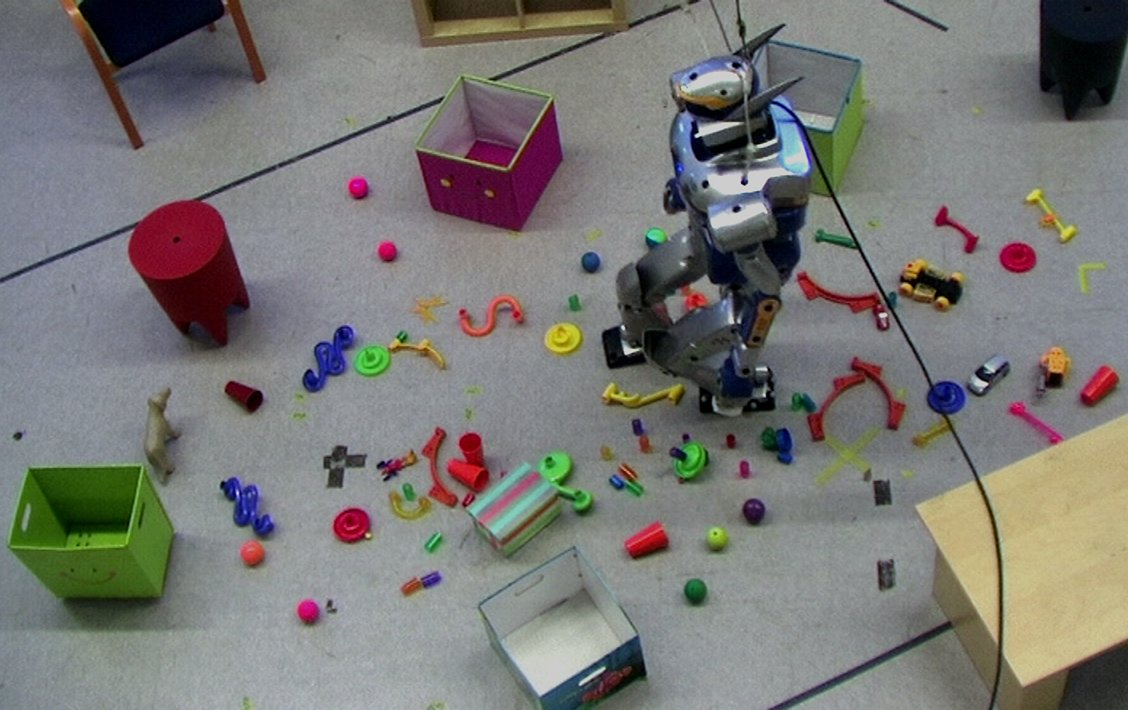
\includegraphics[width=\textwidth]{src/chap2-suivi-trajectoire/demo.jpg}
  \end{center}
  \caption{HRP-2 walking in a cluttered environment while avoiding
    obstacles. The final position is reached with a precision of $\pm
    3\mathrm{cm}$. The final error is the consequence of both noise in
    the robot position estimation and drifts in the two last steps
    which happen too late to be not compensated. \label{fig:scenario}}
\end{figure}
%
%
%
Secondly, the new step is validated. The decision is based on the
relative movement of the first corrected foot. Let consider that, for
instance, the next moving foot is the left one. The original left foot
position is \mbox{$s \in \text{SE}(2)$}, the new corrected left foot
position is \mbox{$s' \in \text{SE}(2)$}. The relative position of the
original and new foot is computed. If the $y$ component of the result
is positive, the new step is accepted. In practice, it means that the
step is ``pushed'' away and will not induce an auto-collision. On the
opposite, with the right foot, the step is accepted if the $y$
component is negative.
%
%
If a correction is invalidated, another one is computed during the
next double support phase. In practice, the estimated error during the
next step will be close to the current estimation, in particular the
sign (i.e. direction) of the error will remain the same. As the flying
foot will change the delayed correction has a high probability of
being accepted.
%
%
This naive system has been empirically validated. However, it prevents
some valid corrected steps. In the future, this will be replaced by a
fast on-line steps validation algorithm described by
\cite{10icra.perrin}.

\section{Résultats expérimentaux}\label{exp}


The proposed method has been validated on HRP-2 using the following
scenarii: the robot walks in a narrow and constrained environment
while stepping over obstacles. The trajectory length is
$2.5\mathrm{m}$ and is executed in approximately $40\mathrm{s}$.
%
%
This setup demonstrates that the execution using this control scheme
is precise and reliable. The robot reaches its goal position with an
error of a few centimeters whereas open loop control schemes is off by
more than a meter. Moreover, the control scheme is reliable: during
the movement, the localization precision can change, the robot
position tracking can fail\ldots The control scheme is designed to be
robust toward these situations.
%
%
This experiment uses the pattern generator described by
\cite{10icra.perrin} and the stack of tasks formalism
\cite{09icar.mansard} to implement the control scheme. The pattern
generator provides reference trajectories for the center of mass and
the feet. Trajectory following tasks for these particular bodies are
then inserted into the control framework. Computing the control such
as the tasks are satisfied is then realized by the solver.
%
%
This experiment video is available on the
web (\mbox{\url{http://youtu.be/cUZ0nNiPs70}}). Fig.~\ref{fig:scenario}
provides an overview of the scenario: the robot starts on the right
side and walks toward the left side.
%
%
%The final position precision depends on the localization precision and
%the steps difficulty. In the proposed scenario, there is no occlusion
%in order to ensure us a good localization. On the opposite, the long
%steps as the one executed on this movement are prone to large
%execution errors.
In this context, the planned final position is
reached with a precision of $\pm 2 \mathrm{cm}$. This trajectory has
been executed five times consecutively with any obstacle collision.
Using a different footsteps sequence with smaller steps, the planned
position can be reached with an error lower than $1 \mathrm{cm}$.


\subsection{De la génération à l'exécution, de la simulation à la réalité}
\subsection{Architecture naïve, boucle ouverte, d'exécution}
\subsection{Fermeture de la boucle d'exécution}

\section{Résultats expérimentaux}

\section{Prospectives}

\chapter{Primitives de mouvement}
\label{chap:primitive}

\epigraph{Vous n'avez qu'à marcher de vertus en vertus.}{Jean
  Racine\\\emph{Britannicus}}
\clearpage

\section{Problématique}

\lettrine[lines=2, lraise=0.1, nindent=0em, slope=-.5em]%
{L}{e} chapitre précédent a introduit la possibilité d'asservir une
trajectoire de marche sur un robot humanoïde. Cependant, les tâches
accomplies par les robots humanoïdes ne se limitent pas à la
locomotion et il est intéressant de se demander s'il est possible de
combiner aux tâches de navigation d'autres tâches asservies par les
données capteurs afin de réaliser des comportements complexes. De
manière indirecte, la question qui se pose ici est celle de la limite
à placer entre d'une part raisonnement numérique et d'autre part
raisonnement logique. Ce problème récurrent de la robotique et pour
lequel il n'existe pas, de consensus au sein de la communauté trouve
ici une solution élégante. En effet, un contrôleur fondé sur le
paradigme de la pile de tâches\index{pile de tâches} ne se limite pas
à une description d'objectifs ou de contraintes robotiques dans des
espaces plus naturels que l'espace des configurations ou l'espace
cartésien, il ouvre surtout la voie à des mécanismes de supervision
décidant à quel moment insérer telle ou telle tâche à un niveau de
priorité donné. La pile de tâches réalise donc la jonction entre d'une
part, le monde du calcul numérique puisque la finalité du système est
de calculer la commande du système et d'autre part le monde de la
logique dans lequel les utilisateurs humains souhaitent exprimer leur
\emph{desiderata} au système robotique: va jusqu'à la cuisine,
apporte-moi la bouteille, ouvre la porte, etc. Il est clair que ce
type d'ordre nécessite la résolution d'abstractions et que la logique
mathématique semble être un moyen particulièrement adapté pour y
parvenir. Ces mécanismes de décision de haut niveau sont appelés
``superviseurs'' et ont pour objectif d'instancier et d'orchestrer
tous les composants d'une architecture robotique. Dans le cadre de
notre architecture, il faut donc pouvoir instancier des piles de
tâches à partir d'une description de haut niveau des ordres passés au
robot. Ce chapitre propose un langage de description des tâches
permettant de faire le lien entre représentation logique et
représentation numérique.


Nous allons commencer par détailler l'état de l'Art et en particulier
les autres travaux ayant trait aux architectures robotiques haut
niveau et à l'ordonnancement de tâches ainsi que plus généralement aux
applications robotiques complexes. Dans un second temps, le langage de
description sera décrit et quelques scénarii types seront
démontrés. Enfin, nous nous concentrerons sur les problèmes
d'asservissement posés par les robots humanoïdes avant de conclure.


\section{État de l'Art}


La perception et l'exécution de tâches asservies en robotique
représentent deux domaines particulièrement actifs. Un livre de
référence sur la localisation robotique et le SLAM\index{Simultaneous
  Localization and Mapping (SLAM)}, le domaine lié à la cartographie
et localisation simultanée en robotique est \cite{05thrun}. Les
travaux de navigation en robotique humanoïdes sont plus rares. On peut
citer les travaux de James Kuffner, Joel Chestnutt, Koichi Nishiwaki
-- \begin{CJK*}{UTF8}{min}正西脇 光一\end{CJK*} --
  \cite{05michel.humanoids,05ozawa.smc,03chestnutt.humanoids,02nishiwaki.rsj}
  de l'Université de Freiburg en Allemagne \cite{10osswald.icra}. Dans
  le domaine la vision pour les humanoïdes, l'utilisation de
  l'asservissement visuel a été tenté \cite{10dune.iros} ainsi que des
  techniques de SLAM telles que
  \cite{06stasse.iros,09kwak.humanoids}. Une introduction à
  l'asservissement visuel\index{asservissement visuel} est
  \cite{06chaumette.ram,07chaumette.ram}. La possibilité d'utiliser un
  robot humanoïde pour la modélisation automatique d'objets 3D a
  également été envisagée par \cite{09foisotte.icra,08stasse.ras}. Une
  approche fondée sur la replanification à partir de données vision
  sur HRP-2\index{HRP-2} a également été publiée dans
  \cite{11dang.humanoids}.


\section{Description d'un mouvement robotique complexe}


Décrire le comportement d'une pile de tâches\index{pile de tâches}
revient à décrire deux éléments primordiaux: d'une part les tâches
exprimées dans le solveur et de l'autre les différents changements
d'état de la pile au cours du mouvement. Concernant les
tâches\index{tâche}, il s'agit ici de représenter des fonctions
mathématiques génériques ne présentant pas de point commun permettant
une représentation générique de ces dernières. Par exemple si l'on se
limitait aux fonctions linéaires $\mathbf{A}(t) \mathbf{x} +
\mathbf{b}(t)$, encoder la matrice $\mathbf{A}$ et le vecteur
$\mathbf{b}$ serait envisageable pour un ensemble discret de valeurs
$t$ données. Le cas évoqué est trop contraint pour notre problème et
les modélisations informatiques développées dans le
\autoref{chap:chap1} n'aident pas: elles ont pour but de venir fournir
un modèle pour l'expression d'une fonction mathématique sous la forme
d'un algorithme et non pas sous la forme d'une donnée structurée
pouvant facilement être encodée. Le choix a donc été fait de définir
un ensemble de tâches permettant de réaliser un certain nombre
d'actions intéressantes. Rien n'empêche alors cet ensemble de
``primitives'' d'être étendu au cours du temps mais il nécessite
l'extension du modèle de description défini ici.


La seconde partie est la représentation des changements d'état. Un
changement d'état du solveur survient quand une tâche est: ajoutée,
supprimée ou bien encore quand sa priorité est modifiée. De manière
générale les transitions peuvent être, soit temporelles -- avance de 5
mètres puis saisis la poignée de la porte --, soit logique -- si tu es
à moins de 10 cm de la position finale, arrête-toi --. Pour comprendre
la stratégie choisie, il faut garder à l'esprit que pour réaliser un
scénario complexe certains comportements seront intégrés dans la
boucle temps réel tandis que d'autres -- typiquement les informations
capteurs -- seront traitées à l'extérieur. Les deux catégories
d'événements, temporelle ou logique, ne mettent pas en jeu les mêmes
mécanismes. Les événements temporels sont décidés à l'avance et
doivent être exécutés avec une grande précision pour assurer un
comportement correct du système tandis que les événements logiques
sont le résultat d'un mécanisme de décision externe.

De ce fait, la stratégie adoptée a été de permettre la représentation
de transitions temporelles dans le modèle de description uniquement
tandis que l'on considère que les transitions événementielles, de fait
plus lentes et difficiles à encoder, sont gérées à l'extérieur du
contrôleur par un logiciel décisionnel ayant la possibilité de
regénérer le mouvement s'il devient invalide suite à la réception
d'une nouvelle donnée capteur. De nombreux logiciels adaptés à cette
tâche ont été développés tel que SMACH\footnote{Site web officiel:
  \url{http://www.ros.org/wiki/smach}}.


\subsection{Primitive de mouvement}
\index{primitive de mouvement}

La première tâche a été de définir des primitives de mouvement de
haut niveau. Les primitives proposées sont:
\begin{enumerate}
\item La locomotion\index{locomotion}: mouvement synchronisé des deux
  jambes et du centre de masse du robot pour réaliser un déplacement
  tout en assurant sa stabilité.
\item La manipulation\index{manipulation} et le contact: mouvement
  réalisant le placement d'une partie spécifiée du robot à un
  emplacement donné dans l'espace euclidien. La tâche peut contraindre
  la position et/ou la rotation du corps à positionner.
\item Regard ou asservissement visuel\index{asservissement visuel}: le
  robot doit maintenir un point dans son champ de vision.
\end{enumerate}


\subsection{Primitive de locomotion}

Une tâche de locomotion est définie initialement comme une série de
points de contact à réaliser pour atteindre une position
finale. Chacun des points de contact\index{point de contact} étant
annoté par l'effecteur devant réaliser le contact à cet endroit. À
partir de ces informations, une trajectoire des effecteurs réalisant
les appuis est déduite ainsi que du centre de masse pour préserver
l'équilibre dynamique du système. Afin de pouvoir utiliser les
techniques décrites dans le \autoref{chap:suivi}, nous nous limiterons
à la marche sur un sol plat utilisant le pied gauche et le pied droit
du robot. Le calcul de la trajectoire des effecteurs et du centre de
masse est encore un problème ouvert à l'heure actuelle. Les modèles
simples peuvent être embarqués dans les contrôleurs au prix de
nombreuses simplifications détaillées dans le chapitre précédent
tandis que les modèles les plus compliqués nécessitent une résolution
hors du contrôleur rendant le comportement du système non réactif. Le
chapitre précédent a proposé une stratégie pour fusionner les
avantages des deux approches. Nous considérons ici la totalité de
l'approche développée au cours du chapitre précédent comme une
implémentation d'une primitive de locomotion. En particulier, l'erreur
de positionnement du robot est considérée comme une entrée de la
primitive de mouvement.


\subsubsection{Tâche d'alignement de deux repères}

Cette primitive de mouvement repose principalement sur la définition
d'une tâche où le solveur doit positionner un corps du robot à un
endroit précis à la fois en rotation et en translation. C'est cette
tâche qui va permettre de faire suivre la trajectoire des pieds
notamment.

\begin{figure}
  \begin{center}
    \begin{equation}
      \left (
      \begin{array}{cccc}
        \cline{1-4}
        \multicolumn{1}{|c}{R_{11}} & R_{12} & R_{13} & \multicolumn{1}{|c|}{t_x} \\
        \multicolumn{1}{|c}{R_{21}} & R_{22} & R_{23} & \multicolumn{1}{|c|}{t_y} \\
        \multicolumn{1}{|c}{R_{31}} & R_{32} & R_{33} & \multicolumn{1}{|c|}{t_z} \\
        \cline{1-4}
        0 & 0 & 0 & 1
      \end{array}
      \right )
    \end{equation}
  \end{center}
  \caption{Structure d'une matrice homogène représentant un élément de
    $\text{SE}(3)$: les coefficients $R_{i,j}$, $(i,j) \in \{1,
    \dotsc, 3\}$ forment la matrice de rotation associé à la
    transformation et $\{t_x, t_y, t_z\}$ le vecteur de
    translation. Une matrice de rotation ayant elle-même une forme
    contrainte: elle doit être une matrice orthogonale de déterminant
    1. \label{fig:matrixhomo}}
\end{figure}


Soit $\mathbf{M}, \mathbf{M}^{*} \in \text{SE}(3)^2$
respectivement la position actuelle du corps du robot et la position
de référence à atteindre. On peut alors définir l'erreur de cette
tâche comme:

\begin{equation}\label{eq:featurepoint6d}
  \mathbf{e} = \mathbf{M} (\mathbf{M}^{*})^{-1}
\end{equation}

On remarquera que dans (\autoref{eq:featurepoint6d}), $\mathbf{e}$ est
un élément de $\text{SE}(3)$. Les éléments de $\text{SE}(3)$ peuvent
s'exprimer de nombreuses façons différentes: matrice homogène -- 16
paramètres --, translation et quaternion -- 7 paramètres
--\index{quaternion}, vecteur de rotation -- 6 paramètres --
\index{vecteur (de rotation)}, etc. Il faut garder à l'esprit qu'une
paramétrisation minimale de $\text{SE}(3)$ nécessite six
paramètres. De fait, tout représentation utilisant un espace de
dimension supérieure vient avec un ensemble de contraintes à respecter
car tous les éléments de cet espace de dimension supérieur ne peuvent
faire partie de $\text{SE}(3)$. Par exemple, une matrice homogène a une
structure bien particulière tel qu'illustré sur la
\autoref{fig:matrixhomo}.

De fait, les représentations non minimales ne constituent pas une
solution acceptable pour représenter notre erreur, car elles
provoquent l'insertion de contraintes supplémentaires inutiles dans le
problème d'optimisation. Il faut donc choisir pour représenter
$\mathbf{e}$ une représentation minimale, dans notre cas par une
translation et une rotation autour d'un axe.

En effet, toute rotation peut être représentée par trois paramètres
\mbox{$\mathbf{\theta} = (\alpha, \beta, \gamma) \in \mathbb{R}^3$}. Le
vecteur $(\alpha, \beta, \gamma)$ normalisé représentant l'axe autour
duquel la rotation s'effectue et la norme du vecteur
$|\mathbf{\theta}|$ la quantité de rotation réalisée autour de cet
axe, voir \autoref{fig:utheta}.

\begin{figure}
  \begin{center}
    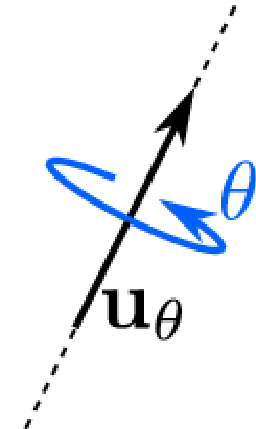
\includegraphics[width=.1\linewidth]{src/chap3-primitive-mouvement/utheta.pdf}
  \end{center}
  \caption{Représentation d'une rotation par un axe de rotation $u$ et
    une quantité de rotation $\theta$. Une représentation minimale à
    trois paramètres est possible en posant: $\theta = |u|$. \label{fig:utheta}}
\end{figure}


Cette représentation est minimale, car la translation est représentée
par trois paramètres et la rotation par trois paramètres:

\begin{equation}
  \mathbf{e} = \left(
  \begin{array}{c}
    t_x\\
    t_y\\
    t_z\\
    \theta_x\\
    \theta_y\\
    \theta_z
  \end{array}
  \right)
\end{equation}

En considérant les trois premiers éléments du vecteur d'erreur ou bien
les trois derniers, on peut restreindre la tâche à positionner le corps
respectivement en translation ou en rotation uniquement.


\subsubsection{Tâche de position du centre de masse}


Le second type de tâche nécessaire pour définir la primitive de
locomotion est la tâche de positionnement du centre de masse.

Cette tâche nécessite la connaissance du poids de tous les corps du
robot $m_i$ où $i \in \mathcal{B}$. $\mathcal{B}$ l'ensemble des corps
du robot. Le centre de masse\index{centre de masse} du robot est alors
défini comme le barycentre des centres de masse de chaque corps:

\begin{equation}
  \mathbf{x} = \frac{1}{\sum_{i \in \mathcal{B}} m_i} \sum_{i \in \mathcal{B}} m_i \mathbf{x}_i
\end{equation}

$\mathbf{x}$ représentation la position du centre de masse du robot et
$\mathbf{x}_i$ la position du centre de masse du corps $i$.

L'erreur de positionnement du centre de masse est alors simplement:

\begin{equation}
  \mathbf{e} = \mathbf{x} - \mathbf{x}^{*}
\end{equation}

La définition de l'erreur ne posant pas de difficulté ici car
$\mathbf{x}$ est un élément de $\mathbb{R}^3$.


\subsubsection{Définition de la primitive de locomotion}

Une tâche de locomotion est par nature critique: un mauvais suivi de
la trajectoire de référence du centre de masse ou bien encore de la
trajectoire des pieds aboutit à une perte de l'équilibre du robot. De
ce fait, établir une priorité entre ces tâches n'a pas de sens. On
préférera donc exprimer ces trois tâches -- pied gauche, pied droit et
centre de masse -- de la façon suivante:

\begin{equation}
  \mathbf{e} = \left(
  \begin{array}{c}
    \mathbf{e}_{\text{pied gauche}}\\
    \mathbf{e}_{\text{pied droit}}\\
    \mathbf{e}_{\text{centre de masse}}
  \end{array}\right)
\end{equation}

Les équations formulées dans cette section peuvent enfin être
paramétrées par le temps courant $t$ afin de permettre une
modification de la valeur de référence notée $\mathbf{M}^*$ ou
$\mathbf{x}^*$ selon les cas et permettre le suivi d'une trajectoire
plutôt que l'atteinte d'une référence constante.


Comme décrit dans le chapitre précédent, l'erreur des tâches décroît
exponentiellement -- dans le cas où la référence reste constante
--. Un suivi suffisamment précis de la trajectoire est alors
réalisable en augmentant suffisamment $\lambda$ le gain associé à la
tâche. Dans la mesure où l'erreur initiale de cette tâche est nulle --
le mouvement commence à la position actuelle du robot -- et varie de
manière continue, la tâche ne génère pas de grandes vitesses
articulaires malgré le gain important.


\subsubsection{Primitive de manipulation}


La primitive de manipulation est une instance directe de la tâche
d'alignement de repères présentée dans la section précédente. Elle
est utilisée pour placer la main à un endroit donné afin de saisir un
objet. Le déplacement d'un bras du robot ne mettant pas en jeu
l'équilibre du robot tant qu'elle se déplace peu rapidement et sans
perturber la tâche de suivi du centre de masse, on peut simplement
corriger l'erreur de positionnement de la main avec une interpolation
linéaire pour amener la main à la position désirée.


\subsubsection{Primitive de regard}


La dernière primitive introduite ici concerne l'asservissement de la
trajectoire du robot afin de préserver des amers dans une zone où
elles sont détectables par les capteurs du robot. Sur le robot HRP-2,
seules des caméras sont à la disposition des utilisateurs et leur
placement dans la tête permet naturellement de définir une tâche de
``regard'' où l'utilisateur souhaite garder un point au centre de
l'image captée par une caméra du robot.

Soit \mbox{$M = (X, Y, Z) \in \mathbb{R}^3$} un point 3D dont les
coordonnées sont définies par rapport à la position de la caméra du
robot et \mbox{$m = (x, y) \in \mathbb{R}^2$} sa projection sur le
plan image de la caméra\index{géométrie projective}. On a alors la
relation suivante:

\begin{equation}
  \mathbf{m} = \left(
  \begin{array}{c}
    x\\
    y
  \end{array}
  \right) = \left(
  \begin{array}{c}
    X / Z\\
    Y / Z
  \end{array}
  \right)
\end{equation}


Une fois de plus l'erreur se définit par la soustraction usuelle:

\begin{equation}
  \mathbf{e} = \mathbf{m} - \mathbf{m}^*
\end{equation}

\begin{figure}
  \begin{center}
    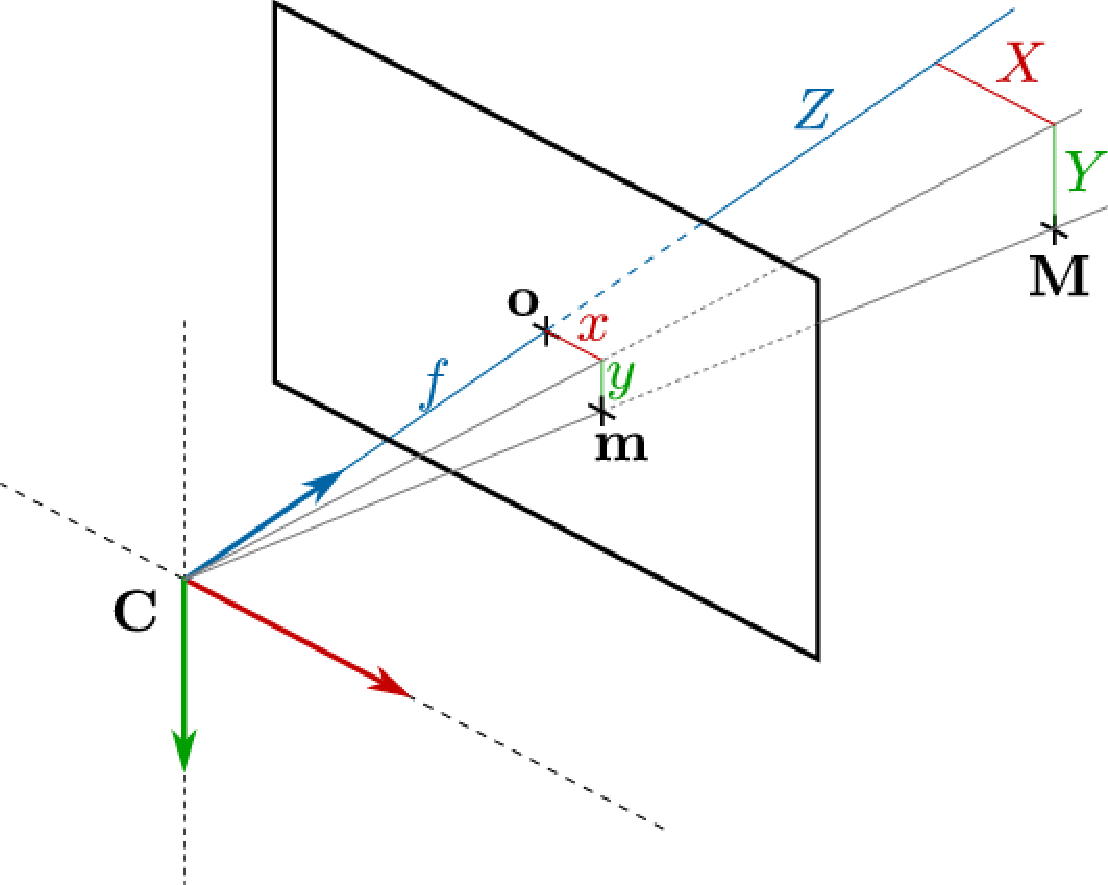
\includegraphics[width=.95\linewidth]{src/chap3-primitive-mouvement/cameraProj.pdf}
  \end{center}
  \caption{Projection du point 3D $M = (X, Y, Z)$ sur le plan image
    d'une caméra idéale. Les coordonées du point projeté sont ici $m =
    (x, y)$. $f$ est la distance focale de la caméra et $C$ le centre
    optique, deux paramètres intrinsèques de la caméra.}
\end{figure}




\subsection{Langage de description}

Le langage de description adopté est le YAML -- Yet Another Markup
Language -- \citep{yaml}\index{Yet Another Markup Language (YAML)}. Le
fichier est divisé en trois parties:
\begin{description}
\item[En-tête] fournissant les méta-informations sur le mouvement,
  notamment sa durée en secondes.
\item[Primitives de mouvement] définissant quelles primitives sont
  jouées et sur quel intervalle, ainsi que la configuration de chaque
  primitive.
\item[Primitives d'asservissement] définissant comment l'erreur de
  positionnement du robot est estimée au fil du temps.
\end{description}


\subsubsection{Primitive de locomotion}
\index{primitive!de locomotion}

Une primitive de locomotion est définie par un ensemble de points de
contacts définis sur la forme d'une pile de pas.

\begin{description}
\item[Intervalle.] Date de début et de fin de la primitive de mouvement.
\item[Empreinte de pas.] Liste des pas à effectuer. Les pas sont
  considérés comme des éléments de $\text{SE}(2)$ dans la mesure où
  l'algorithme de génération de pas fait l'hypothèse d'un sol plan.
\end{description}

Lors du chargement du plan, la génération des trajectoires de pieds et
de centre de masse initiales est réalisée hors ligne de manière
asynchrone. Tant que le calcul n'est pas terminé, il n'est pas
possible de lancer le mouvement.


\subsubsection{Primitive de manipulation}
\index{primitive!de manipulation}

Une primitive de manipulation est définie par un corps et une position
6d de référence. L'objectif est de faire coïncider le corps avec la
position 6d de référence. Cette tâche peut ne considérer que la
rotation ou la translation.

\begin{description}
\item[Intervalle.] Date de début et de fin de la primitive de manipulation.
\item[Corps à considérer.] Nom du corps à considérer. Des noms
  génériques ont été définis tels que: cheville gauche, cheville
  droite, poignet gauche, poignet droit, tête, torse et bassin.
\item[Consigne.] La position de référence vers laquelle le corps doit
  être amené. Il peut être de trois types. Soit statique, le corps
  doit maintenir sa position initiale, soit fixe dans ce cas le corps
  doit atteindre un point prédéterminé de l'espace, soit dynamique
  dans ce cas le corps doit suivre un point mobile.
\end{description}


\subsubsection{Primitive de regard}
\index{primitive!de regard}

La primitive de regard définit comment le robot peut maintenir son
regard vers un point 3D, éventuellement mobile.

\begin{description}
\item[Intervalle.] Date de début et de fin de la primitive de manipulation.
\item[Caméra à considérer.] Nom de la caméra utilisée. En pratique, la
  caméra est définie comme un corps ``virtuel'' du robot et l'on peut
  donc potentiellement aligner n'importe quelle partie du corps du
  robot vers un point donné.
\item[Consigne.] La position de référence vers lequel le corps doit
  pointer. Il peut être de deux types. Soit fixe, dans ce cas le corps
  doit pointer vers un point prédéterminé de l'espace, soit dynamique
  et dans ce cas le corps doit pointer vers un point mobile.
\end{description}


\subsubsection{Asservissement des primitives sur les données capteur}


Une fois la séquence de mouvement définie, il faut encore pouvoir
fermer la boucle sur les données capteur. Dans le cadre d'un mouvement
complexe, une stratégie intéressante est de pouvoir s'asservir
successivement sur plusieurs amers afin de planifier \emph{a priori}
quelle est la ou les amers les plus pertinentes à différents instants.


Soit $\mathcal{L}$ un système de localisation. Un système de
localisation est défini comme une fonction qui à tout instant fournit
une pose estimée d'un corps de référence du robot, dans notre cas le
bassin. On a donc:

\begin{equation}
  \begin{array}{ccc}
    \mathcal{L} : & \mathbb{R} \rightarrow & \text{SE}(2)\\
      & t \mapsto & \mathcal{L}(t)
  \end{array}
\end{equation}

Au cours du mouvement, $n$ systèmes de localisation fournissent une
estimation de la pose du robot. Une fois de plus, cette pose est
théoriquement dans l'espace 3D $\text{SE}(3)$, mais les contraintes
physiques font que seuls trois degrés de liberté doivent être
réellement estimés: $(x, y, \theta) \in \text{SE}(2)$. Ces trois
degrés correspondent à la position 2D de la projection du bassin sur
le sol. De ce fait, l'interpolation de $n$ poses 2D et la moyenne des
poses à la normalisation de l'angle $\theta$ prêt.


On associe à chaque système de localisation une fonction de poids
déterminant l'influence relative des systèmes de localisation dans
l'estimation finale de la pose:

\begin{equation}
  \begin{array}{ccc}
    m_i : & \mathbb{R} \rightarrow & \mathbb{R}\\
      & t \mapsto & m_i(t)
  \end{array}
\end{equation}

La fusion des données pour l'estimation de la pose est donc le
barycentre des poses 2d:

\begin{equation}
  \mathbf{\hat{x}}(t) = \frac{1}{\sum_{i \in n} m_i} \sum_{i \in n} m_i \mathcal{L}_i(t)
\end{equation}

En pratique, chaque système de localisation est représenté de la façon suivante:
\begin{description}
\item[Poids.] en fonction du temps. Il peut, soit être constant, soit
  varier dynamiquement.
\item[Erreur.] de positionnement en fonction du temps. Elle est fournie
  par un système de localisation externe.
\end{description}


\section{Scénarii de mouvements}


Nous allons voir ici plusieurs exemples de mouvements décrits en
utilisant le langage de description introduit dans la section
précédente. L'objectif est à la fois de démontrer la généricité de
l'approche par plusieurs scénarii différents ainsi que sa mise en
\oe uvre pratique.


\subsection{Locomotion simple}

Le premier scénario consiste en le déplacement du robot le long d'une
pile de pas prédéterminée pendant 20 secondes. La description
complète du plan est fournie par la \autoref{fig:plan_locomotion_simple}.

\begin{figure}
  \begin{center}
\begin{verbatim}
duration: 20 # durée complète du mouvement (secondes)

# Éléments de mouvement
motion:
  # Primitive de locomotion
  - walk:
      interval: [0, 20] # Date de début et de fin de la primitive

      # Pile de pas
      footsteps:
      - {x: 0.15, y: -0.19, theta: 0.}
      - {x: 0.15, y: +0.19, theta: 0.1}
      # etc.
\end{verbatim}
  \end{center}
  \caption{Plan de mouvement pour une séquence de marche non asservie.\label{fig:plan_locomotion_simple}}
\end{figure}

La marche est effectuée en boucle ouverte et l'erreur d'exécution
n'est pas compensée. Chaque pas est exprimé relativement au pas
précédent. Le corps effectuant chaque contact peut être déduit de la
séquence d'empreinte de pas: si la translation en $y$ du premier pas
dispose d'un signe négatif, le premier pas est effectué avec le pied
droit, sinon avec le pied gauche. L'alternance pied gauche/pied droit
à chaque pas est ensuite implicite.


Il n'y a pas, à ce niveau de vérification de la faisabilité des
pas. C'est le rôle du planificateur de s'assurer préalablement à la
génération du plan de mouvement que la séquence est réalisable.

\begin{figure}
  \begin{center}
    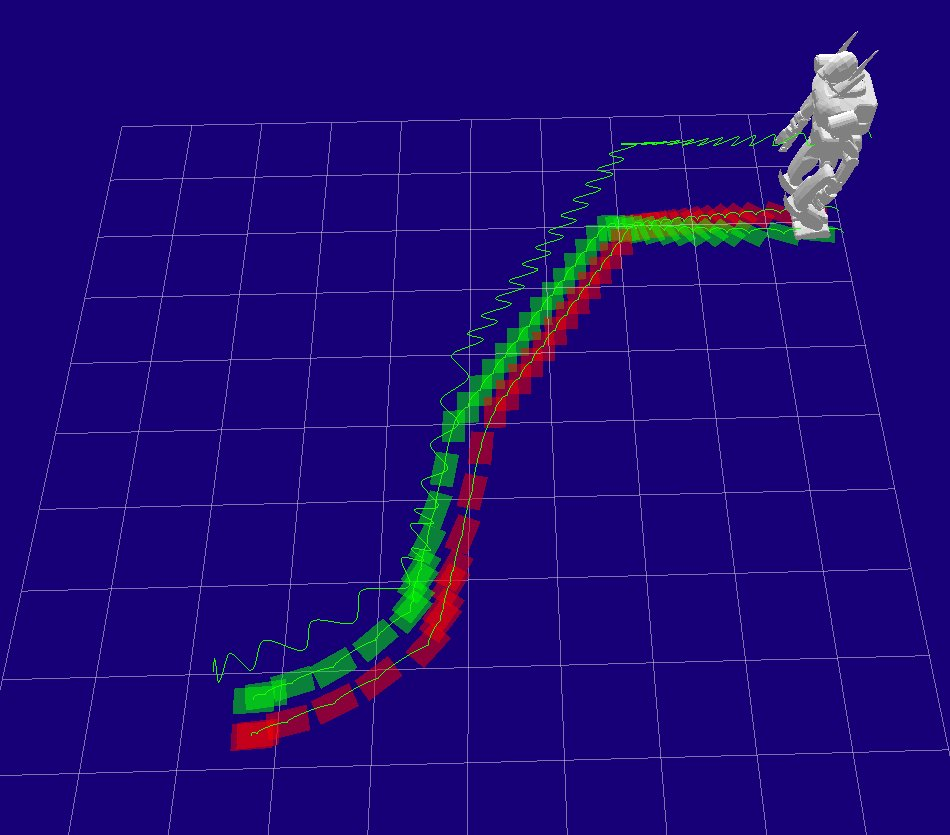
\includegraphics[width=.95\linewidth]{src/chap3-primitive-mouvement/footsteps1.jpg}
  \end{center}
  \caption{Exemple de pile de pas à partir de laquelle une primitive
    de locomotion peut être calculée.}
\end{figure}


\FloatBarrier

\subsection{Locomotion asservie}

On peut se demander désormais comment asservir la locomotion en
utilisant un composant de localisation. La
\autoref{fig:plan_locomotion_asservie} fournit une version alternative
du plan précédent ajoutant la correction de pas introduite dans le
\autoref{chap:suivi}.

\begin{figure}
  \begin{center}
\begin{verbatim}
duration: 20 # durée complète du mouvement (secondes)

# correction maximum autorisée sur un pas (x, y en mètre, theta en radians)
maximum-correction-per-step: {x: 0.02, y: 0.02, theta: 0.05}

# Éléments de mouvement
motion:
  # Primitive de locomotion
  - walk:
      interval: [0, 20] # Date de début et de fin de la primitive

      # Pile de pas
      footsteps:
      - {x: 0.15, y: -0.19, theta: 0.}
      - {x: 0.15, y: +0.19, theta: 0.1}
      # etc.

# Asservissement des tâches
servoing:
  # Asservissement via le système de capture de mouvements.
  - mocap:
      weight: 1.
      tracked-body: left-ankle
      perceived-body: left-foot
\end{verbatim}
  \end{center}
  \caption{Plan de mouvement pour une séquence de marche asservie sur
    un système de localisation -- ici un système de capture de
    mouvement --.\label{fig:plan_locomotion_asservie}}
\end{figure}

La seconde partie du plan décrit que l'erreur de positionnement
provient d'un unique système de localisation. Dans ce cas, un système
de capture de mouvement. Plusieurs systèmes de localisation ont été
testés pour fournir une estimation de la position du robot au cours du
mouvement:

\begin{description}
\item[Capture de mouvement.] Ce système permet une localisation
  quasi-parfaite permettant de s'abstraire de la plupart des problèmes
  de perception.
\item[Suivi d'un objet.] Un système réalisant le suivi d'un objet dans
  l'image captée par une caméra du robot et reconstituant sa
  position 3D peut également être utilisé. Dans ce cas, on suppose
  l'objet fixe dans le monde et on en déduit la position du robot.
\item[SLAM.] Les techniques de SLAM -- Simultaneous Localization and
  Mapping -- permettent de cartographier l'environnement tout en
  fournissant une estimation de la position actuelle du robot. La
  carte enregistrée permet d'assurer une localisation sans dérive
  quelque soit la longueur du mouvement à condition de pouvoir
  identifier des amers précédemment détectées régulièrement le long
  du mouvement.
\end{description}

\begin{figure}
  \begin{center}
\begin{verbatim}
duration: 20 # durée complète du mouvement (secondes)

# correction maximum autorisée sur un pas (x, y en mètre, theta en radians)
maximum-correction-per-step: {x: 0.02, y: 0.02, theta: 0.05}

environment:
  - object:
      name: table
      planned:
        position:
          x: 1.75
          y: 0.3
          z: -0.3
          rx: 0.
          ry: 0.
          rz: 2.

# Éléments de mouvement
motion:
  # Primitive de locomotion
  - walk:
      interval: [0, 20] # Date de début et de fin de la primitive

      # Pile de pas
      footsteps:
      - {x: 0.15, y: -0.19, theta: 0.}
      - {x: 0.15, y: +0.19, theta: 0.1}
      # etc.

# Asservissement des tâches
servoing:
  # Asservissement via le système de capture de mouvements.
  - visp:
      interval: [0, 20] # Date de début et de fin de l'élément d'asservissement.
      weight: 1.
      object-name: table
      position: /tracker_mbt/resultTransform
      camera-velocity: /tracker_mbt/camera_velocity
      frame-name: cameraBottomLeft
\end{verbatim}
  \end{center}
  \caption{Plan de mouvement pour une séquence de marche asservie sur
    un système de suivi d'objet.}
\end{figure}

\begin{figure}
  \begin{center}
\begin{verbatim}
duration: 20 # durée complète du mouvement (secondes)

# correction maximum autorisée sur un pas (x, y en mètre, theta en radians)
maximum-correction-per-step: {x: 0.02, y: 0.02, theta: 0.05}

# Éléments de mouvement
motion:
  # Primitive de locomotion
  - walk:
      interval: [0, 20] # Date de début et de fin de la primitive

      # Pile de pas
      footsteps:
      - {x: 0.15, y: -0.19, theta: 0.}
      - {x: 0.15, y: +0.19, theta: 0.1}
      # etc.

# Asservissement des tâches
servoing:
  # Asservissement via le système de localisation externe (SLAM).
  - control-ros:
      weight: 1.
      topic: /error
      signal: error
\end{verbatim}
  \end{center}
  \caption{Plan de mouvement pour une séquence de marche asservie sur
    un algorithme de SLAM. En pratique, dans ce cas l'évaluation de
    l'erreur est totalement effectuée hors du contrôle.}
\end{figure}

\FloatBarrier

\subsection{Scénario d'atteinte avec équilibre quasi statique}

Dans ce scénario, le robot place son poignet a un point prédéterminé
tout en préservant la position de son centre de masse. Le plan de
mouvement est détaillé dans la \autoref{fig:plan_atteinte}.

\begin{figure}
  \footnotesize
  \begin{center}
\begin{verbatim}
duration: 10 # durée complète du mouvement (secondes)

motion:
# Fixe la position des pieds.
  - task:
      # Date de début et de fin de la primitive.
      interval: [0, 10]
      # Type de la tâche: positionnement d'un corps.
      type: feature-point-6d
      # Corps à positionner (cheville gauche).
      operational-point: left-ankle
      # Gain de la tâche.
      gain: 1.
      # Consigne de la tâche: aucun mouvement.
      reference: static
      # Contrainte en translation *et* rotation.
      translation: on
      rotation: on
  - task:
      # Date de début et de fin de la primitive.
      interval: [0, 10]
      # Type de la tâche: positionnement d'un corps.
      type: feature-point-6d
      # Corps à positionner (cheville droite).
      operational-point: right-ankle
      # Gain de la tâche.
      gain: 1.
      # Consigne de la tâche: aucun mouvement.
      reference: static
      # Contrainte en translation *et* rotation.
      translation: on
      rotation: on
# Fixe la position du centre de masse.
  - task:
      # Date de début et de fin de la primitive.
      interval: [0, 10]
      # Type de la tâche: positionnement du centre de masse.
      type: feature-com
      # Gain de la tâche.
      gain: 1.
      # Consigne de la tâche: aucun mouvement.
      reference: static
      # Degré de liberté supplémentaires déverrouillés.
      extra-unlocked-dofs: [18., 19.] # HRP-2 chest dofs.

# Tâche d'atteinte.
  - task:
      # Date de début et de fin de la primitive.
      interval: [0, 10]
      # Type de la tâche: positionnement d'un corps.
      type: feature-point-6d
      # Corps à positionner (poignet droit).
      operational-point: right-wrist
      # Gain de la tâche.
      gain: 7.5
      # Consigne: position finale du poignet droit.
      reference: {x: 0.4, y: -0.3, z: 1.1}
      # Contrainte en translation uniquement.
      translation: on
      rotation: off
\end{verbatim}
  \end{center}
  \caption{Plan de mouvement pour une tâche d'atteinte.\label{fig:plan_atteinte}}
\end{figure}

Contrairement à la tâche de locomotion qui est totalement encapsulée
dans une primitive peu paramétrable, le scénario d'atteinte nécessite
la définition manuelle des tâches. Quatre tâches sont définies ici:
deux pour maintenir les pieds à leur place, une pour maintenir le
centre de masse à sa position initiale et une dernière qui génère le
mouvement du poignet droit.

Les tâches associées aux pieds et au centre de masse possèdent un gain
faible, car l'erreur a une erreur nulle initialement. Inversement, la
tâche associée au poignet droit a une erreur maximum initialement et
donc une vitesse maximum. Le gain permet alors de contrôler la vitesse
de réalisation de la tâche et donc, de manière indirecte, la vitesse
de déplacement du bras.

\FloatBarrier

\subsection{Scénario d'asservissement visuel de la tête}

La dernière primitive de mouvement considérée ici permet d'asservir le
regard du robot sur la position d'un point 3D, soit fixe, soit mobile
et estimé par un système externe. Le plan correspondant est la
\autoref{fig:plan_asservissement_complet}.

\begin{figure}
  \footnotesize
  \begin{center}
\begin{verbatim}
duration: 25 # durée complète du mouvement (secondes)
# correction maximum tous les deux pas
maximum-correction-per-step: {x: 0.04, y: 0.04, theta: 0.1}

environment:
  - object:
      name: table
      planned:
        position:
          x: 1.75
          y: 0.3
          z: -0.3
          rx: 0.
          ry: 0.
          rz: 2.

motion:
  # Primitive de locomotion
  - walk:
      interval: [0, 20] # Date de début et de fin de la primitive

      # Pile de pas
      footsteps:
      - {x: 0.15, y: -0.19, theta: 0.}
      - {x: 0.15, y: +0.19, theta: 0.1}
      # etc.

  # Asservissement de la tête
  - visual-point:
      interval: [0, 25]
      gain: 1.
      object-name: table
      frame-name: cameraBottomLeft

servoing:
  - visp:
      weight: 1.
      object-name: table
      position: /tracker_mbt/resultTransform
      frame-name: cameraBottomLeft
\end{verbatim}
  \end{center}
  \caption{Plan de mouvement pour une tâche de marche avec
    asservissement de la tête.\label{fig:plan_asservissement_complet}}
\end{figure}

\FloatBarrier

\section{De la difficulté à localiser un robot humanoïde}
\label{sec:chap3_localisation}


Plusieurs séries d'expérimentation ont été réalisées sur le robot
HRP-2 afin de tester le comportement des algorithmes de localisation
utilisant des capteurs embarqués.


\begin{figure}
  \begin{center}
    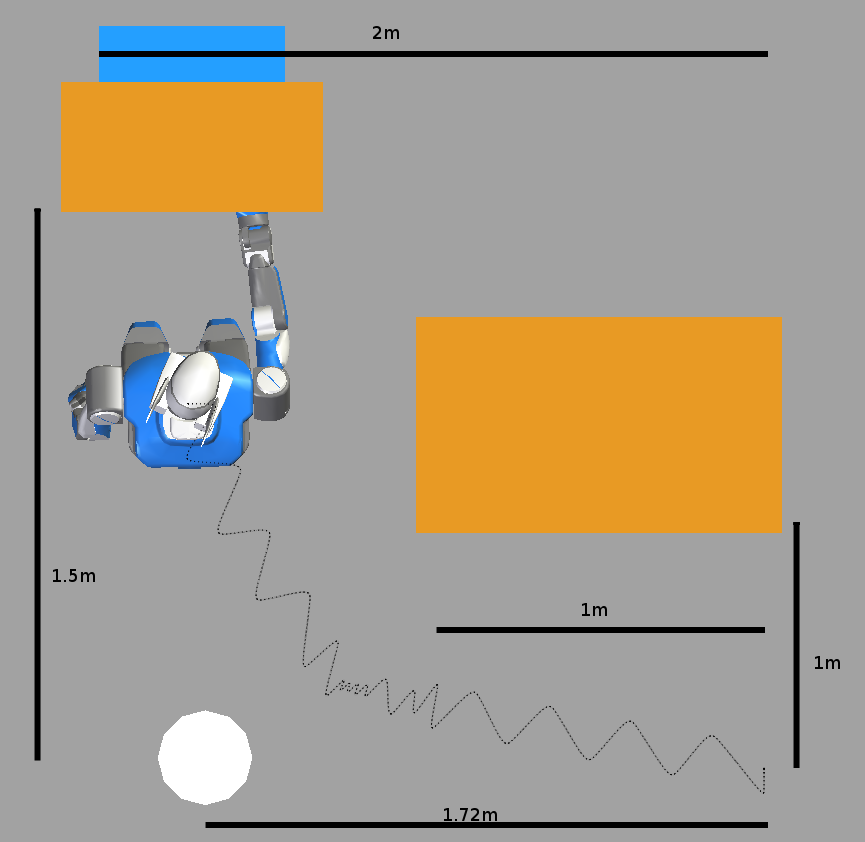
\includegraphics[width=.75\linewidth]{src/chap3-primitive-mouvement/dimensions.png}
    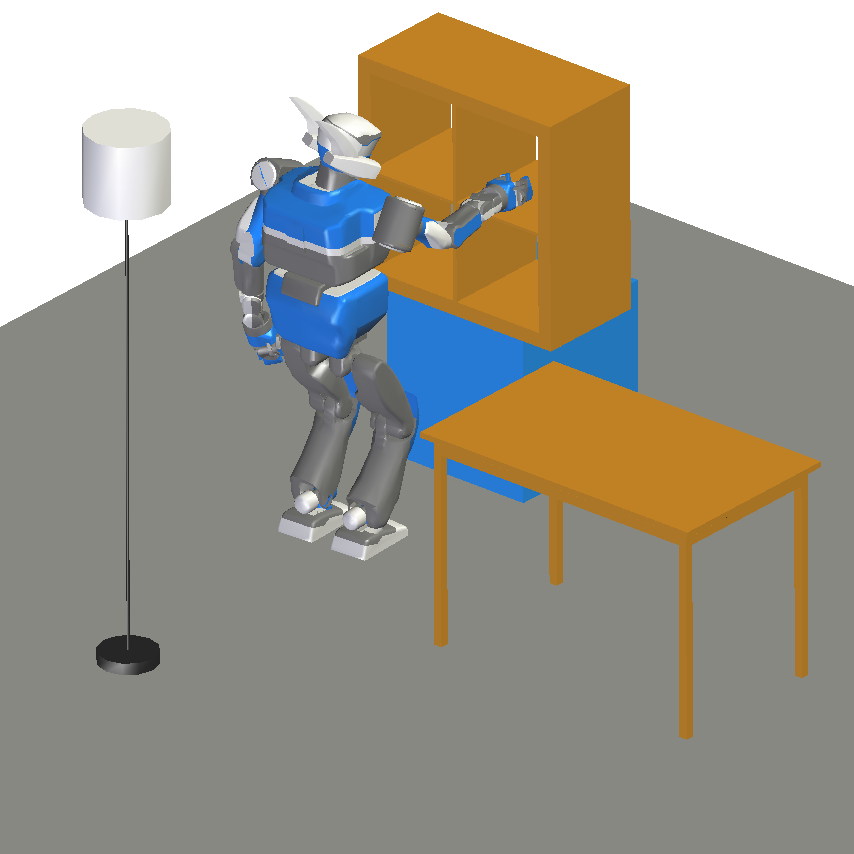
\includegraphics[width=.75\linewidth]{src/chap3-primitive-mouvement/trajectory-8.png}
  \end{center}
  \caption{Description de l'expérimentation: le robot part de la
    droite de l'image et progresse vers l'étagère située à gauche pour
    y déposer une balle. \label{fig:scenario_visu}}
\end{figure}



Le scénario proposé est le suivant: HRP-2\index{HRP-2} contourne un
obstacle, passe entre deux objets, et va poser une balle sur une
étagère. La longueur de la trajectoire de marche -- 2 mètres environ
-- et le nombre de pas génèrant une dérive suffisante pour qu'une
exécution de ce scénario échoue en boucle ouverte. En effet, passer
son bras dans une étagère est un mouvement contraint particulièrement
sensible à la position d'arrivée du robot. Une petite erreur dans le
positionnement du robot à la fin de la trajectoire engendrera une
grande erreur dans la position finale du
poignet. La \autoref{fig:scenario_visu} illustre le scénario.
L'objectif ici est d'utiliser les caméras embarquées pour construire
une carte de l'environnement puis pour localiser le robot. La
stratégie adoptée ici n'est pas du SLAM -- Simultaneous Localization
and Mapping --\index{Simultaneous Localization and Mapping (SLAM)}
dans la mesure où les images permettant de construire la carte sont
traitées hors ligne. On réalise donc un premier mouvement sans
correction afin d'acquérir une séquence d'images permettant de
construire la carte puis on utilise cette carte pour localiser le
robot durant les expérimentations suivantes. La qualité du résultat
est ensuite validée en utilisant un système de capture de mouvement.


Durant les expériences, le module de localisation a fourni une
estimation de la position du robot à 16\hertz. Les images ont une
résolution de 320x240 pixels. L'ordinateur sur lequel fonctionne le
composant de localisation est un
\mbox{Intel\textregistered~Core\texttrademark 2 CPU T7200 @ 2.00GHz}
avec 2 Gb.\ de RAM.


\subsection{Analyse de la précision du système de localisation}

La précision finale du système est illustrée par la
\autoref{fig:scenario_visu_precision}. On peut y observer une erreur à
la fin de la trajectoire d'environ 0.2 mètres en
translation. Plusieurs raisons peuvent expliquer ces mauvais
résultats:
\begin{enumerate}
\item Carte non métrique et absence de fermeture de boucle,
\item Passage dans des zones où la carte est peu dense ou dans des
  zones ne possédant que peu d'information visuelle,
\item Flexibilité du robot et/ou mauvaise identification de certains paramètres,
\end{enumerate}


Le premier point pouvant amener à une mauvaise estimation de la
localisation du robot est l'absence de fermeture de boucle. Les
techniques de localisation utilisant les informations visuelles
peuvent être divisées en deux catégories: odométrie
visuelle\index{odométrie visuelle} et localisation
``globale''. L'odométrie visuelle observe les changements entre deux
images aux temps $t_{n-1}$ et $t_n$ afin d'estimer la vitesse de la
caméra entre les deux images. Cette vitesse est ensuité intégrée pour
calculer le mouvement de la caméra. Par conséquent, il se produit une
dérive temporelle qui empêche toute tentative de localisation sur le
long terme en utilisant cette technique. Inversement, les algorithmes
utilisant une carte peuvent identifier les amers déjà détectés
auparavant et stabiliser le système. Une limite de ce mouvement est
qu'il n'est pas facile pour le système de reconnaître des amers déjà
identifiés. Il s'en suit une dérive dans l'estimation de la position
du robot.


Le second problème concerne l'environnement en lui-même: à la fin du
mouvement, le robot se trouve face au meuble ce qui rend les images
captées par les caméras vides de tout amer permettant d'effectuer
correctement la localisation. Ce problème ne peut expliquer que
partiellement la mauvaise estimation dans la mesure où l'occlusion des
caméras n'intervient qu'à l'extrême fin du mouvement.


Le dernier point pouvant amener à une mauvaise estimation de l'erreur
est lié à la mauvaise modélisation de la chaîne cinématique du
robot. Une première erreur est liée à la présence, au niveau des
chevilles du robot, d'une flexibilité passive pouvant être modélisé
sous la forme de trois ressorts: deux autorisant un mouvement en
rotation et un troisième un déplacement en translation, c'est à dire
autorisant une compression de la cheville lors de la marche. Ce
dispositif a été conçu pour absorber les chocs et protéger le capteur
de force situé dans la cheville mais insère trois degrés de liberté
non modélisés et surtout non mesurables, car dépourvu
d'encodeur. Cette déformation au niveau de la cheville est donc
ignorée dans les calculs ce qui amène à un biais sur la position
relative du pied et de la tête du robot. Ce biais est d'autant plus
critique dans ce cas que c'est la position des points de contact que
l'on essaie de corriger. Une seconde source d'erreur est la
calibration de la position de la caméra dans le robot. Les
imprécisions de la conception du robot, du système de fixation des
caméras rendent nécessaire le calcul de la position relative de la
caméra par rapport au corps auquel il est fixé, dans notre cas la
tête. Un procédé de calibration des paramètres
extrinsèques\index{paramètres extrinsèques (d'une caméra)} a donc été
mis en place pour estimer ces paramètres. Ces derniers ont été validés
en reprojetant le modèle du robot dans l'image comme illustré par la
\autoref{fig:reprojection_modele_vision}.


\subsection{Résultats de la localisation utilisant la vision sur le robot humanoïde HRP-2}

L'ensemble de ces facteurs rend la réalisation d'un algorithme de
localisation embarqué sur HRP-2\index{HRP-2} délicat. Pour réaliser
une tâche de manipulation, une précision de l'ordre du centimètre est
souvent nécessaire. Or, les mauvaises performances du système de
localisation engendrent un bruit dans le positionnement du robot qui
peut rendre l'exécution de tâches précises délicates. Dans le scénario
choisi, la tâche peut être réalisée avec succès pour certains essais,
mais le taux d'échec restant très fort, cette méthode ne peut pas
constituer une boîte noire permettant de manière automatique de
réaliser un mouvement asservi. Une façon de résoudre le problème
serait de corriger la position du bras. En effet, entre la caméra et
le bras, la chaîne cinématique est bien identifiée. On voit donc ici
que l'approche consistant à avoir plusieurs systèmes de localisation
simultanément se justifie en pratique. Un composant de localisation
``global'' tel que celui utilisé ici permet de rendre la navigation
robuste sans toutefois être suffisant pour les tâches de
manipulation. Pour ces dernières, d'autres stratégies doivent être
envisagées comme la détection dans l'image de l'objet à attraper pour
asservir la position de la pince. On voit ici que plus qu'une
localisation parfaite sur le long terme, il est plus critique pour nos
scénarii d'avoir des algorithmes de localisation locaux assurant une
erreur minimale à la fin de la réalisation de la tâche. Les
algorithmes réalisant une localisation sur le long terme étant plutôt
destinés à alimenter les algorithmes de planification que les
algorithmes de contrôle nécessitant une haute précision sur la pose
estimée du robot.




\begin{figure}
  \begin{center}
    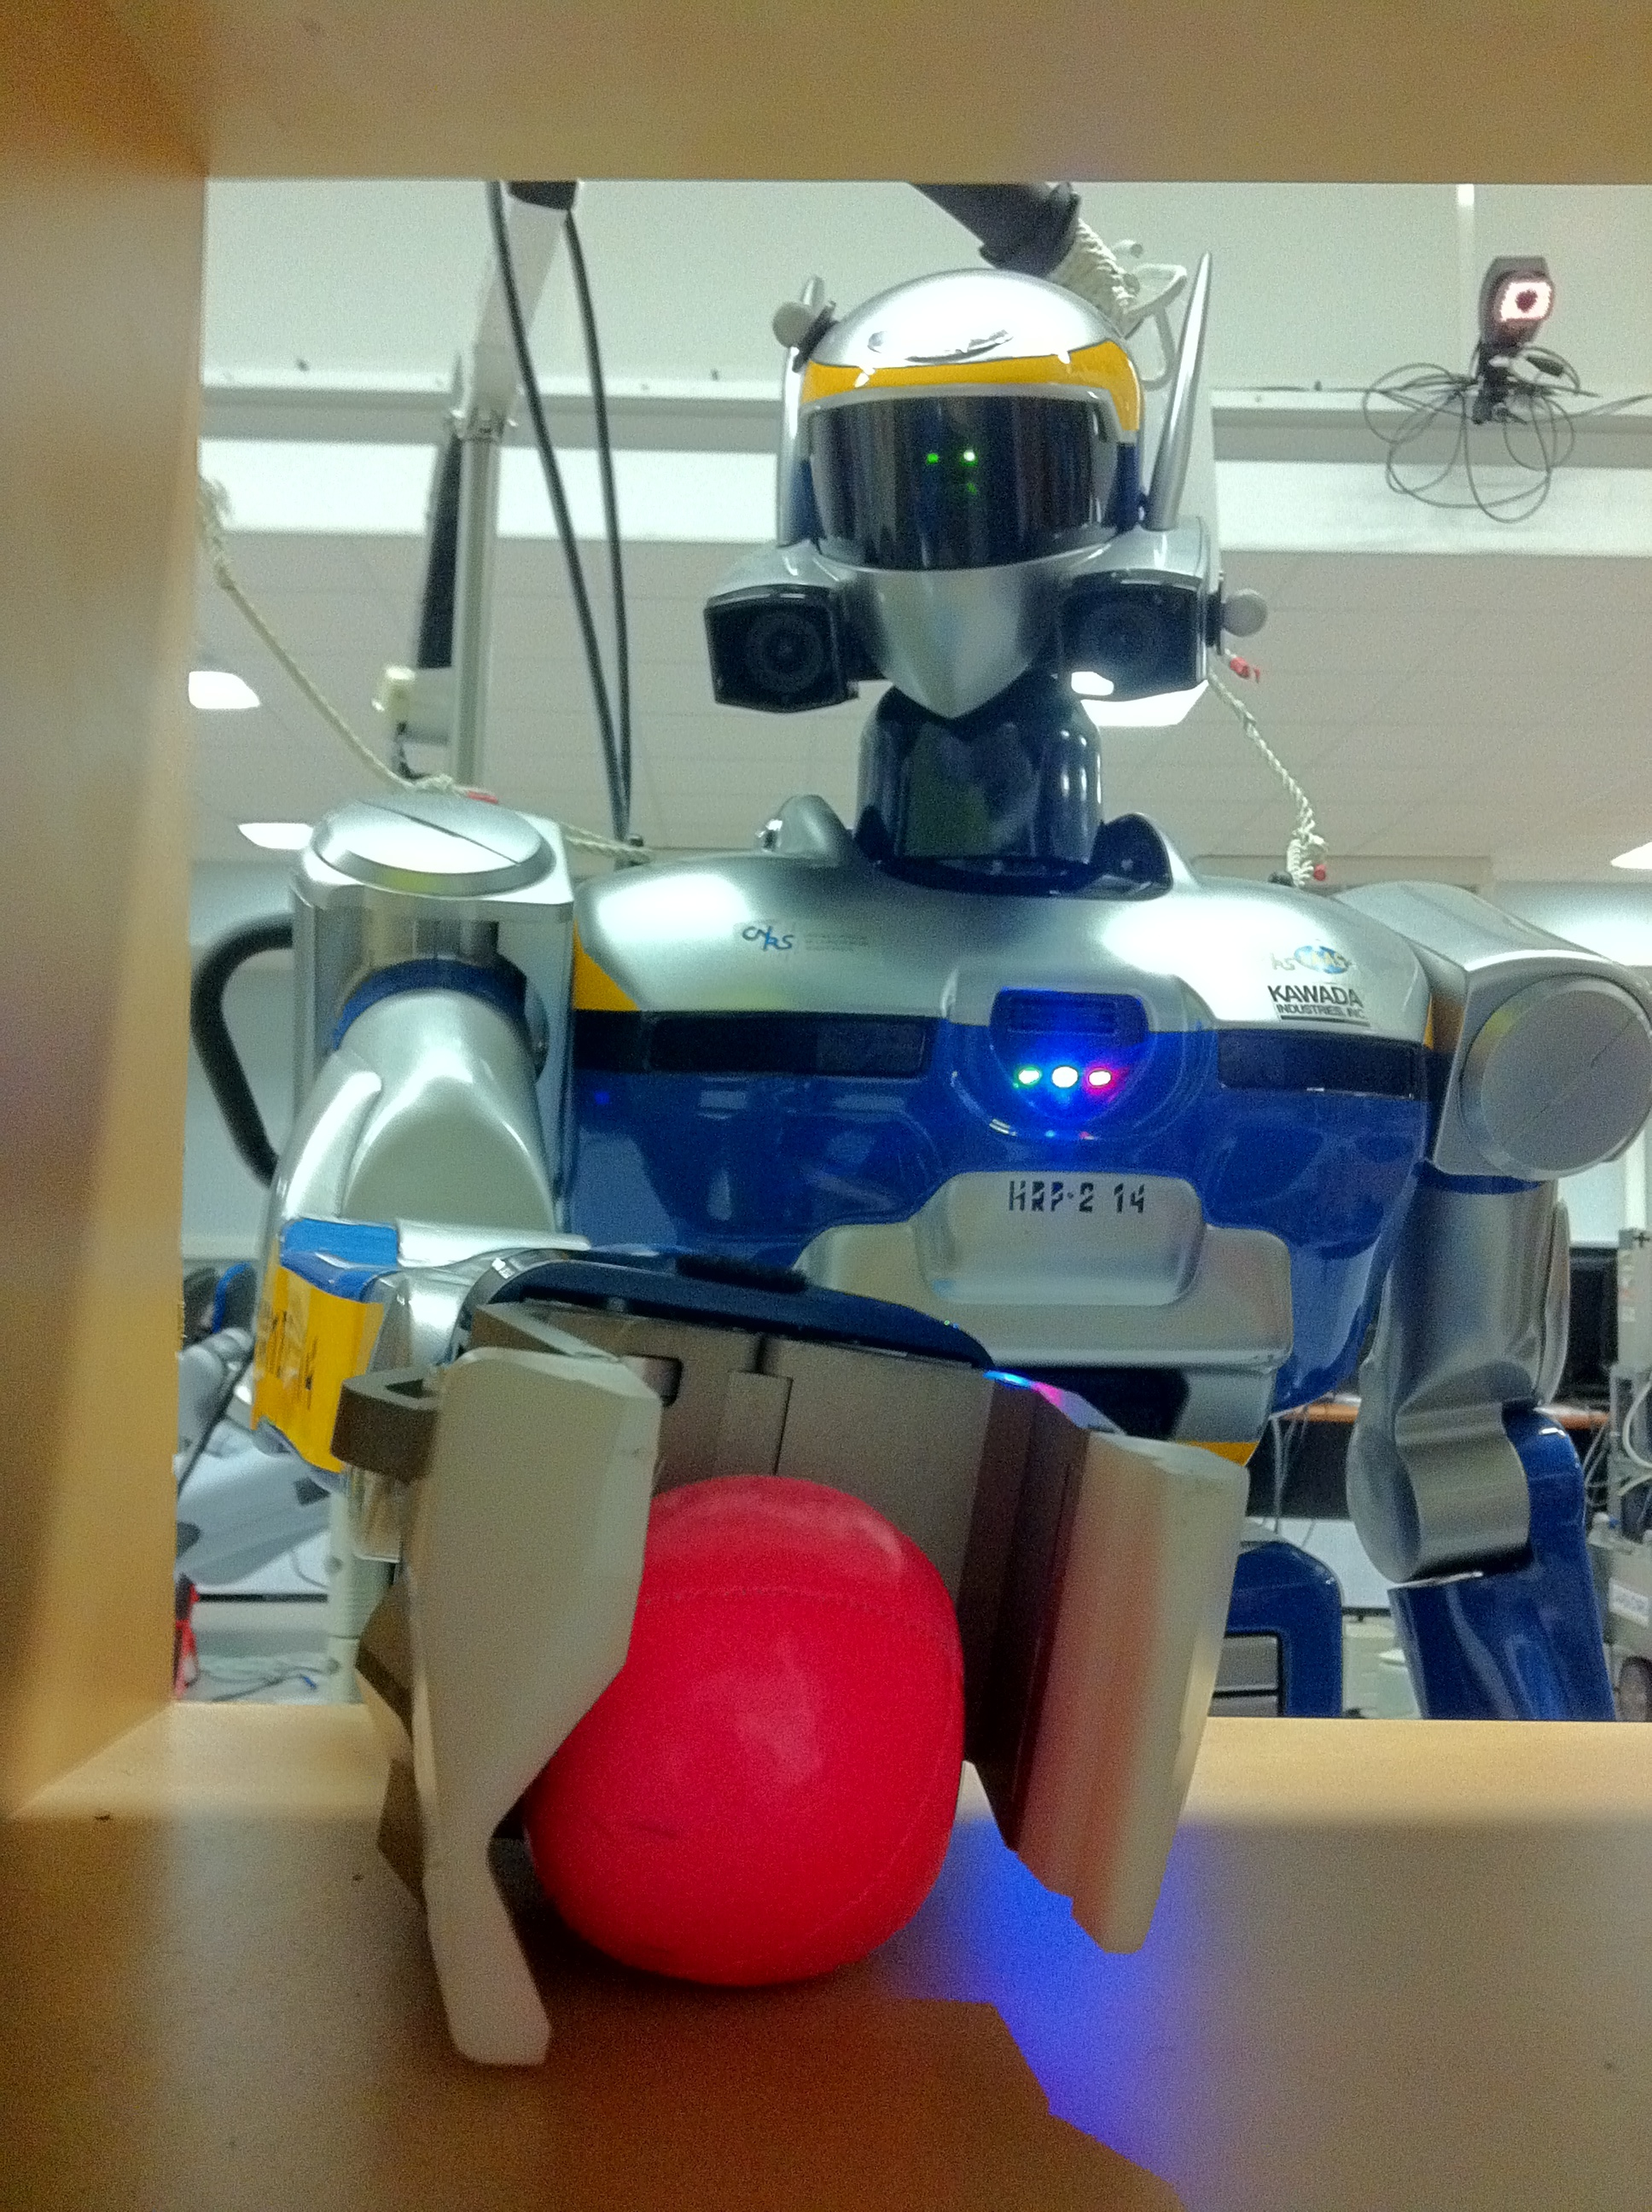
\includegraphics[width=.95\linewidth]{src/chap3-primitive-mouvement/demo1.jpg}
  \end{center}
  \caption{HRP-2 place une balle dans une étagère (I).}
\end{figure}

\begin{figure}
  \begin{center}
    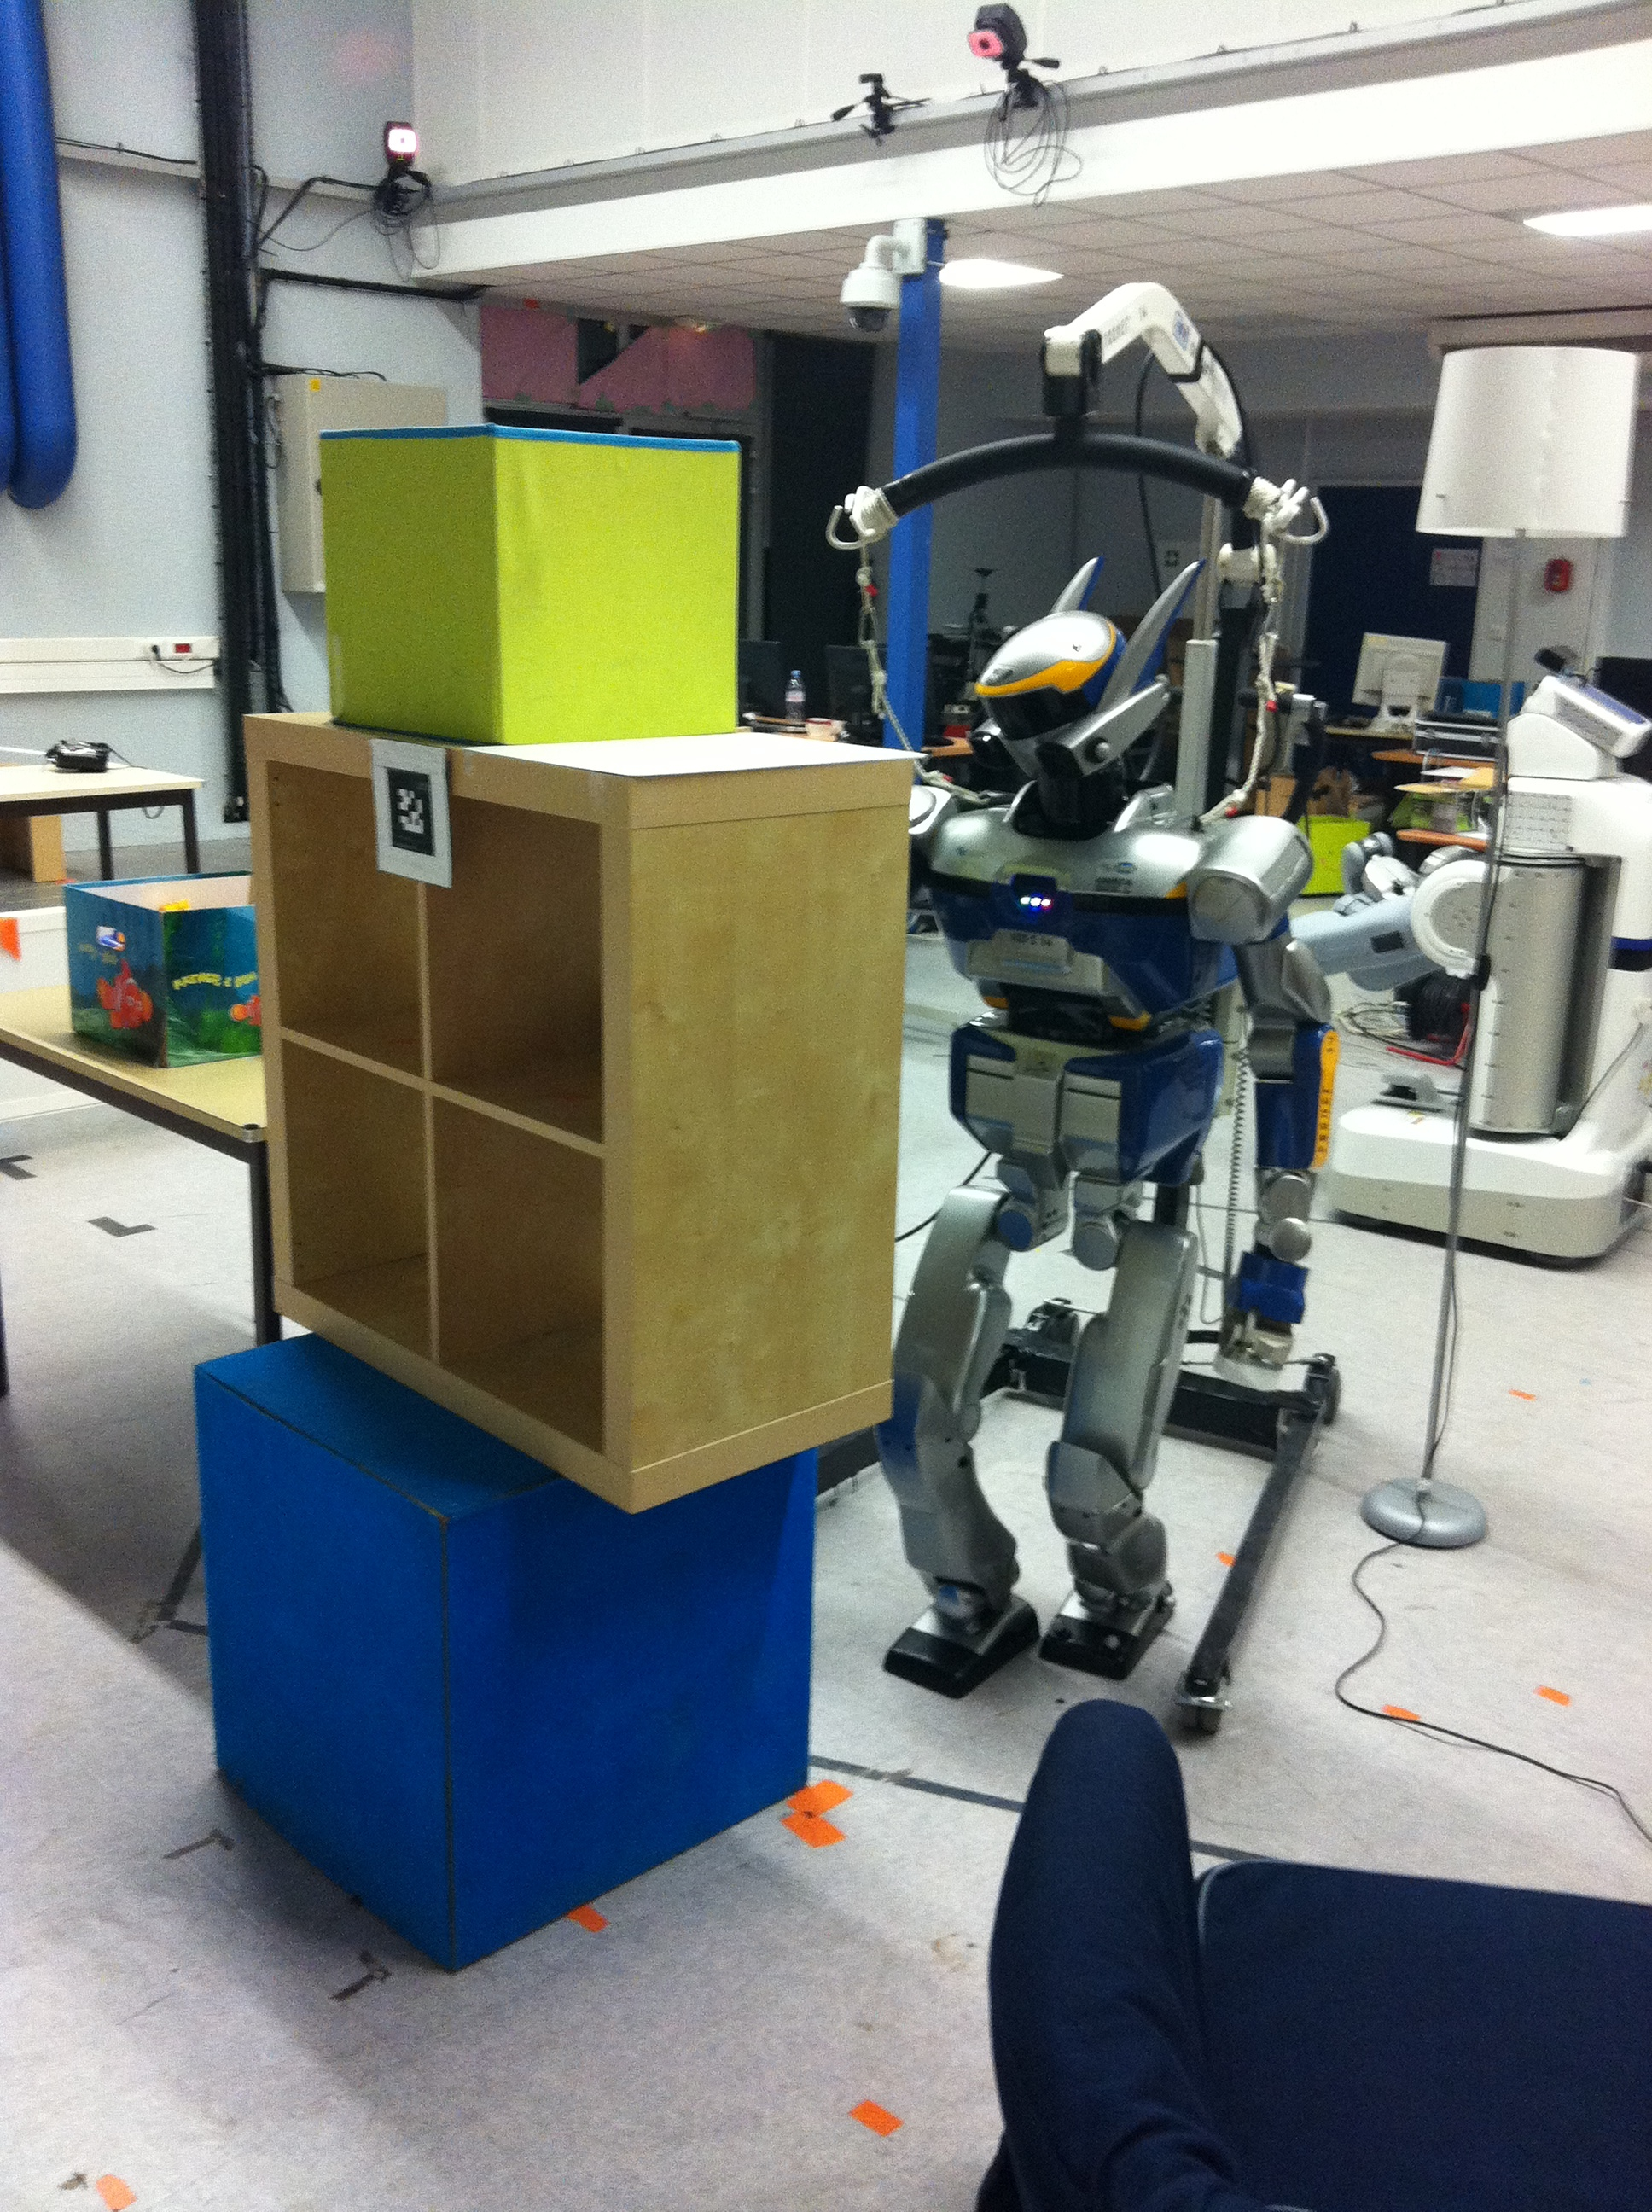
\includegraphics[width=.95\linewidth]{src/chap3-primitive-mouvement/demo2.jpg}
  \end{center}
  \caption{HRP-2 place une balle dans une étagère (II).}
\end{figure}


\begin{figure}
  \begin{center}
    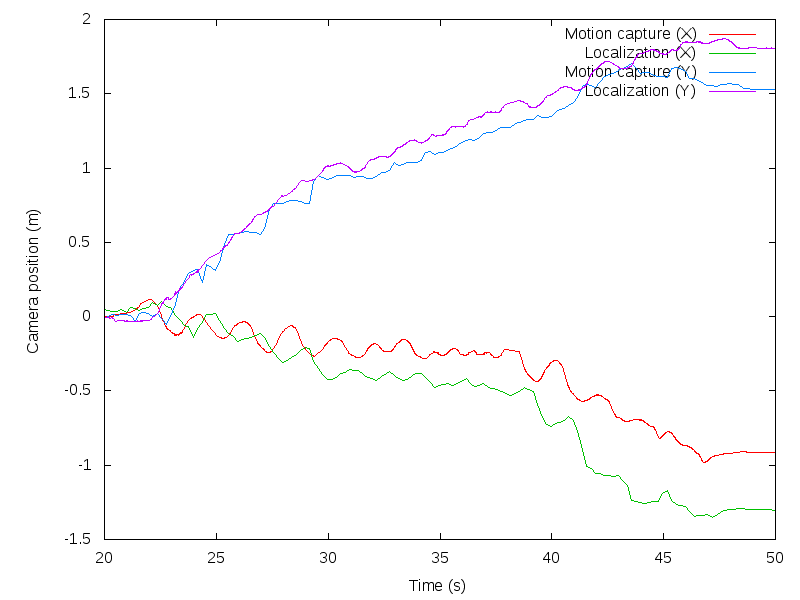
\includegraphics[width=.95\linewidth]{src/chap3-primitive-mouvement/mocap.png}
  \end{center}
  \caption{Précision de l'algorithme de SLAM par rapport au système de
    capture de mouvemement. \label{fig:scenario_visu_precision}}
\end{figure}

\begin{figure}
  \begin{center}
    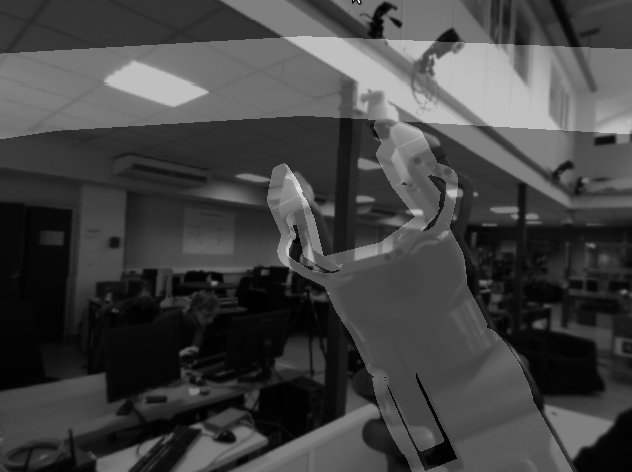
\includegraphics[width=.95\linewidth]{src/chap3-primitive-mouvement/calibextrinsic.jpg}
  \end{center}
  \caption{Reprojection du modèle du robot dans l'image captée par une
    caméra embarquée pour valider la calibration des paramètres de
    cette dernière. \label{fig:reprojection_modele_vision}}
\end{figure}


\section{Conclusion}

Pour continuer à explorer l'expression de plans de mouvement, il
faudrait donc intégrer de nouveaux algorithmes de localisation dédiés
à l'asservissement d'une tâche spécifique plutôt que d'envisager le
problème comme un bloc unitaire. La seconde partie des travaux reste
d'intégrer directement dans la phase de planification une étape de
planification des asservissements. L'idée est de planifier le
mouvement tel que le robot privilégiera le passage dans des zones où
la qualité de la localisation est maximale. En particulier, la
trajectoire de la tête sera calculée afin de laisser les amers
détectables le plus longtemps possible utilisables. Ce planificateur
pourra alors générer la partie asservissement du plan de mouvement
automatiquement. L'intégration de ces deux éléments reste un objectif
clé afin de pouvoir asservir n'importe quel mouvement sur un robot
humanoïde de manière automatique.

\chapter{Applications robotiques complexes}
\label{chap:integration}

\epigraph{\foreignlanguage{USenglish}{The belief that complex systems
    require armies of designers and programmers is wrong. A system
    that is not understood in its entirety, or at least to a
    significant degree of detail by a single individual, should
    probably not be built.}}{Niklaus Wirth}
\clearpage

\lettrine[lines=2, lraise=0.1, nindent=0em, slope=-.5em]% {C}{e}
chapitre est dédié à la conception d'architectures robotiques
complexes permettant la validation de nouveaux algorithmes robotiques.
Les précédents chapitres ont montré une progression d'une approche qui
est dédiée purement à la génération de trajectoires par l'utilisation
d'outils d'optimisation numérique vers un l'exécution de scénarios
dont la complexité a augmenté incrémentalement. Ce passage de la
génération de trajectoire sans ``conscience'' de ce qu'est un système
évoluant dans le monde réel vers une application robotique réelle ne
va pas sans la nécessité d'intégrer et de maîtriser une grande variété
d'algorithmes et de technologies tout en les utilisant conjointement
afin de finalement, atteindre un objectif de haut niveau. Ce chapitre
va donc décrire l'architecture qui a été mise en place sur le robot
humanoïde HRP-2 afin de réaliser un ensemble de scénario
expérimentaux, certains faisant partie intégrante des chapitres
précédents et d'autres étant le résultat de travaux de recherche
disjoints, mais prenant appui sur l'architecture développée ici. Ce
chapitre tente également de fournir des conseils et une méthodologie
pour la conception d'applications robotiques. Une partie de la
méthodologie décrite dans ce chapitre est issue des recommandations
classiques de l'ingénierie logicielle, mais il est également
nécessaire de prendre en considération les particularités de la
robotique.

\section{Architecture}


Les systèmes robotiques complexes peuvent être décomposés en trois
grandes parties:

\begin{enumerate}
\item La couche de perception\index{perception} qui analyse
  l'environnement autour du robot et construit un modèle du monde,
\item La couche de décision\index{décision} qui va tenter de résoudre
  la tâche donnée au système tout en prenant en compte l'état actuel
  du monde,
\item La couche action\index{action} qui va utiliser les capacités du robot pour
  réaliser la tâche proprement dite. En particulier, les capacités
  d'actionnement du robot sont ici utilisées pour impacter le monde
  environnant.
\end{enumerate}


Cette architecture largement décrite par la littérature est encore
d'actualité pour les robots humanoïdes. En effet, cette catégorisation
est issue de la présence dans un système robotique de boucles lentes
et de boucles rapides. Typiquement, la prise de décision est un
processus lent -- qui peut prendre plusieurs secondes --, la
planification de mouvements est un exemple de ce type de processus. Au
contraire, la couche action contrôlant les actionneurs nécessite le
plus souvent d'être extrêmement réactive et impose des contraintes
importantes en terme de temps réel. Il faut pouvoir garantir que la
boucle de contrôle peut être évaluée à une fréquence donnée ce qui
contraint à la fois le type d'algorithmes pouvant être exécuté dans
cette boucle ainsi que le volume de donnée pouvant être traité. Enfin,
la couche de perception est, elle, en général plus lente que le
contrôle et dépendante de la vitesse à laquelle les capteurs du robot
peuvent fonctionner. Qui plus est, il arrive parfois que les capteurs
acquièrent des données plus vite qu'elles sont traitées et certaines
données sont alors ignorées silencieusement. On a donc ici trois types
de comportements extrêmement différents.


Les couches perception et décision nécessitent une grande puissance de
calcul pour pouvoir assurer une réactivité suffisante. Cette puissance
de calcul est parfois déportée sur un ordinateur spécifique. Par
exemple dans le cadre du robot HRP-2, deux ordinateurs sont
embarqués. Le premier est dédié à la boucle de contrôle temps réel et
est relié aux actionneurs tandis que le second est relié aux capteurs
-- ici les caméras embarquées -- et support les algorithmes de
décision et de perception.


Afin de découpler les algorithmes robotiques, chaque algorithme est
implémenté au sein d'un composant robotique\index{composant
  robotique}. En pratique, un composant robotique est un processus --
c'est-à-dire un programme indépendant -- pouvant communiquer avec un
ou plusieurs autres composants. La distribution des calculs sur
plusieurs ordinateurs rend nécessaire la définition d'un protocole de
transmission des données afin de pouvoir assurer une bonne
interprétation de ces dernières au sein d'un environnement
informatique hétérogène. Un exemple est la représentation des nombres
au sein des architectures informatiques: une architecture peut être
dit ``big endian''\index{big endian (architecture)} ou ``little
indian''\index{little endian (architecture)} selon l'ordre dans lequel
les bits représentants le nombre sont enregistrés. Dans une
architecture ``big endian'' les nombres ayant les poids les plus forts
sont contenus en mémoire en premier tandis que les architectures
``little endian'' adoptent un ordre inverse. Ce type de problème rend
nécessaire la définition d'un modèle de communication entre
composants.


Les architectures robotiques autorisent généralement la communication
entre deux composants, ou n\oe uds, soit sous une forme discrète, soit
sous une forme continue. La forme discrète est appelée
``service''\index{service} et se modélise sous la forme d'un appel de
fonction distant. Un algorithme est généralement divisé en fonctions,
ces dernières formant des blocs logiques pouvant être combinés entre
eux pour réaliser des comportements de plus haut niveau. Les services
fournissent un moyen d'appeler une fonction qui ne sera non pas
exécutée au sein du processus courant, mais dans un autre processus,
voire sur un autre ordinateur de manière transparente. La difficulté
résidant dans le passage des arguments et la transmission du
résultat. Il est nécessaire que cette fonction soit définie selon des
règles particulières afin de s'asssurer que les données peuvent être
correctement transmises via le réseau sans compromettre leur
intégrité. Cette phase dîte de ``sérialisation''\index{sérialisation}
assurer le fonctionnement de ces mécanismes dans des environnements
informatiques hétérogènes. La seconde forme de communication sert à
modéliser des flux de donnée continus et est appelée
``topic''\index{topic}. Dans ce cas, le premier composant communique a
un ou plusieurs autres des données mises à jour régulièrement. De la
même façon, un processus de sérialisation est nécessaire pour assurer
que les données peuvent être transmises même si un ou plusieurs autres
composants ne font pas partie du même processus ou ne sont pas
exécutés sur le même ordinateur.


De nombreux outils logiciels implémentent ces mécanismes sous
différentes formes. Le choix réalisé sur le robot humanoïde HRP-2 a
été d'utiliser ROS -- Robotics Operating System --\index{ROS}, un
projet communautaire initié par la société californienne Willow
Garage\index{Willow Garage}. Le mécanisme de communication ainsi
qu'une grande partie de la modélisation du processus de perception se
fonde sur les outils développés dans le cadre de ce projet. Les
sections suivantes vont détailler les différents composants
fonctionnant sur le robot humanoïde HRP-2.



\subsection{Contrôle}

Sous le terme de ``contrôle'' est désigné le composant robotique
chargée de calculer la commande qui sera envoyée aux actionneurs. Il
est impératif que cet ordre déterminant le prochain état que les
servomoteurs du système vont s'efforcer d'atteindre soit envoyé à une
fréquence fixe. Sur le robot humanoïde HRP-2, la fréquence de la
boucle de contrôle est de 200$\hertz$, il faut donc que la boucle de
contrôle ne mette pas plus de 5ms pour être évaluée. Les noyaux des
systèmes d'exploitation multitâches ne fournissent pas de garantie
forte sur la réactivité des logiciels exécutés. Il est donc nécessaire
d'utiliser des noyaux dédiés afin d'assurer que la boucle de contrôle
soit exécutée en permanence à la fréquence voulue. Ces contraintes
impliquent que les composants de contrôle se doivent d'être aussi
minimaux que possible et sont souvent monolithiques. À ce sujet, les
contrôleurs robotiques partagent une grande ressemblance avec les
noyaux des systèmes d'exploitation. Ils assurent également la sûreté
du système: une mauvaise commande envoyée aux moteurs peut, très
souvent, entraîner la destruction des actionneurs.

Dans le cas de systèmes robotiques complexes, il est courant d'avoir
plusieurs contrôleurs exécutés successivement au sein de la boucle de
contrôle. Ainsi l'architecture d'HRP-2 se fonde sur un système de
plug-in permettant de charger des contrôleurs ``à chaud''. Chaque
contrôleur est alors modélisé par une machine à état très simple FIXME
FIG. Le contrôleur passe alors dans les états suivants:

\begin{itemize}
\item Initialisation sans contrainte de temps réel
\item Initialisation avec contrainte de temps réel
\item Exécution
\item Destruction avec contrainte de temps réel
\item Destruction sans contrainte de temps réel
\end{itemize}

Le passage d'un état à l'autre se réalisant dans l'ordre, avec un
bouclage sur la phase d'exécution autant qu'il soit nécessaire.


L'architecture de contrôle est divisée en trois contrôleurs:
\begin{description}
\item[Pile de tâches\index{pile de tâches}] À partir d'un ensemble de
  tâches, la résolution de la pile de tâches est calculée dans la
  boucle de contrôle afin de calculer la commande à envoyer aux
  moteurs. HRP-2 étant commandé en position, la commande envoyée
  correspond à la position articulaire des différents joints du
  système.
\item[Stabilisateur\index{stabilisateur}] HRP-2 intègre un mécanisme
  d'absorption passif des chocs appelé ``silent blocks''\index{silent
    block}. Ce système passif intègre au niveau des chevilles une
  compliance difficile à modéliser et à prendre en compte dans le
  calcul de la commande. La centrale inertielle du robot permettant
  d'estimant l'attitude du bassin, le stabilisateur peut déduire
  l'état des flexibilités des chevilles et, à l'aide des capteurs de
  force placés dans les chevilles, réaliser un asservissement
  bas-niveau sur la trajectoire du ZMP désiré. Ce mécanisme permet de
  compenser la modélisation sommaire de la dynamique réalisée, par
  exemple, par l'utilisation du modèle simplifié du ZMP ainsi que des
  éventuelles erreurs de modélisation de la structure du robot. Ce
  système compense les erreurs de suivi du ZMP en modifiant les
  valeurs des articulations des jambes du robot.
\item[Communication] Le dernier élément communique vers l'extérieur
  les informations liées au contrôle du robot tel que les commandes
  envoyées, réellement exécutées -- c'est-à-dire après stabilisation
  --, ainsi que les sorties des capteurs tels que la centrale
  inertielle et les capteurs de force placés aux chevilles et poignets
  du robot.
\end{description}


On notera que pour le dernier contrôleur, la communication réseau
étant implémentée en TCP/IP\index{TCP/IP}, il n'est pas possible de
garantir le temps pris par l'envoi des données et il est donc
impossible d'envoyer des données en TCP/IP\index{TCP/IP} sans
compromettre la boucle temps réel. Cette partie est donc divisée en
plusieurs fils d'exécution non bloquants afin de garantir la sûreté du
système. En pratique, chaque ``topic'' permettant la communication de
données vers l'extérieur publie les données dans un fil d'exécution
séparé et non temps réel. Le fil d'exécution\index{fil d'exécution}
temps réel lui tente de copier la donnée vers une variable lue par ce
fil d'exécution. Si ce dernier est en train d'y accéder et qu'elle
n'est pas accessible, un verrou protège l'accès à la ressource et la
publication de la donnée pour ce tour de boucle est ignorée. En
pratique, la communication vers l'extérieur est réalisée à 20$\hertz$. En
moyenne, une donnée sur dix est donc envoyée afin d'éviter d'engorger
le système.


En terme de conception, les composants nécessitant un rafraichissement
à une vitesse supérieure doivent être intégrés à la boucle de
contrôle. Pour les autres données, il faut pouvoir, via le schéma de
calcul, pouvoir utiliser les informations temporelles attachées aux
données capteur envoyées pour gérer de manière consistante le retard
inhérent à toute donnée provenant d'une architecture distribuée.


\subsection{Vision}


La vision est l'élément central de la perception sur un robot
humanoïde. Elle est caractérisée par une particularité qui détermine
tous les traitements qui lui sont affectés: les caméras produisent des
quantités de données extrêmement importantes. De ce fait, il est
important d'éviter de réaliser des traitements inutiles et il faut
également éviter au maximum les copies. Le traitement des images est
souvent réalisé en série: on acquiert une image, on la convertit, on
la rectifie et puis on cherche à en tirer des informations de plus
haut niveau. Ces traitements en série se modélisent particulièrement
bien sous la forme d'un tuyau dans lequel les images passent les unes
après les autres. La stratégie classique de la robotique tend alors à
dédier un composant par traitement afin de garder un système
modulaire, mais la taille des données rend cela difficile. En effet,
si chaque composant vit dans un processus différent, il est nécessaire
de passer par des mécanismes de mémoire partagée afin d'éviter les
copies en mémoire. ROS a choisi une seconde stratégie en offrant la
possibilité d'agglomérer plusieurs composants dans un seul
processus. La sérialisation devient donc totalement inutile au prix
d'une plus grande complexité dans l'écriture des n\oe uds et d'une
forme d'insécurité: si un problème advient dans n'importe lequel de
ces composants, il provoquera l'arrêt de la totalité du
système. Cependant, les traitements étant effectués en série, devoir
relancer tous les traitements en cas de panne n'amène pas de perte
significative de qualité de service.


Nous allons donc désormais nous attacher à développer les différents
composants de vision qui ont été utilisés sur le robot HRP-2 et
agglomérés dans la chaîne de traitement des images du robot.


\paragraph{Acquisition des images}

L'acquisition des images est réalisée par un composant communiquant
avec le pilote FireWire. Les quatre caméras du robot sont des Flea2 du
fabricant PointGrey. Ces caméras sont reliées à un FireWire IEEE
1394b\index{FireWire IEEE 1394b}. Les limitations du bus ne permettent
pas l'acquisition des données sur les quatre caméras simultanément, on
peut donc passer de la paire de caméras grand-angle à la seconde paire
de caméras. La première paire est dédiée à la perception de
l'environnement au détriment de la précision tandis que la seconde
dispose d'un champ plus resserré, adapté à la manipulation fine
d'objets notamment.

Les images acquises utilisent un encodage de Bayer\index{Bayer
  (encodage de)}. Cet encodage, nommé du nom de son inventeur, Bryce
E. Bayer chercheur au sein de la société Kodak, réalise l'encodage
d'images couleurs sur 8 bits au lieu des 24 bits habituellement
nécessaires pour représenter les trois canaux utilisés pour encoder
les trois couleurs primaires: rouge, vert et bleu. Cet encodage encode
la couleur verte sur 50\% du volume de donnée totale tandis que bleu
et rouge représentent 25\% chacun. Cette prépondérance du vert est
fondée sur la plus grande sensibilité au vert des cônes, les
photorécepteurs présents au fond de l'\oe il.


\paragraph{Traitements des images}

Une fois les images acquises, il est important de les convertir dans
un espace colorimétrique\index{espace colorimétrique} adapté à leur
traitement. La première étape est donc de dématricer les images
encodées en Bayer vers des images monochromatiques ou couleurs 24 bits
dans l'espace RGB habituel. Dès maintenant, un branchement s'effectue
entre les traitements utilisant les images couleur et les traitements
utilisant les informations de luminance uniquement. Afin de fournir
une expérience unifiée, les deux ``topics'' sont créés, mais les
traitement ne sont effectués qu'à partir du moment où au moins un
client se connecte à ce dernier. On peut donc offrir une large palette
de possibilités sans mettre à mal les performances du système. Le
dématriçage\index{dématriçage} des images encodées en Bayer
reconstruit les couleurs manquantes en interpolant grâce à la couleur
des pixels adjacents. Plusieurs techniques ayant des coûts de calcul
différents existent selon les cas: interpolation bilinéaire,
interpolation bicubique ou bien encore rééchantillonage de
Lanczos\index{Lanczos (rééchantillonage de)}.


La seconde étape consiste à rectifier les images. Nous nous
intéresserons d'abord au cas de la rectification\index{rectification}
monoculaire. Dans ce cas, l'objectif de ce procédé est de se ramener
au cas de la caméra parfaite dit
``pinhole''\index{sténopé}\index{modèle de caméra
  pinhole|see{sténopé}} -- ou sténopé en français -- où la projection
du point 3d $P$ sur le plan image donne un point 2d $p$ qui correspond
parfaitement à la projection de ce dernier en passant par le point
focal de la caméra $C$: $p_x = P_x / P_z$ et $p_y = P_y / P_z$ où
$P_x, P_y, P_z$ sont les coordonnées du point dans l'espace 3D et
$p_x, p_y$ les coordonnées 2D du point $p$ dans le plan image. Ce
n'est pas jamais totalement le cas en réalité: le plan image n'est pas
un plan parfait, l'axe optique n'est jamais exactement au centre de la
caméra et les objectifs réalisent une distorsion\index{distorsion} des
rayons lumineux captés. Pour pouvoir raisonner sur ce modèle idéal, on
va donc traiter l'image afin qu'elle puisse être considérée comme
provenant d'un capteur idéal ayant le comportement d'un sténopé, à la
différence de la caméra réelle. Il faut pour cela calibrer la caméra
et identifier ses paramètres intrinsèques\index{paramètres
  intrinsèques (de caméra)}: $(u_0, v_0)$ la position de l'axe optique
dans l'image, $(p_x, p_y)$ la taille des pixels permettant de réaliser
la conversion des pixels vers les mètres et un ensemble de paramètres
permettent d'identifier la distorsion de l'image originale. Plusieurs
modèles sont décrits par la littérature, mais dans notre cas une
estimation de la distorsion radiale\index{distorsion radiale} est
suffisante pour compenser l'utilisation d'un objectif grand-angle.


Le processus de calibration est réalisé en utilisant une mire que l'on
place à différents endroits relativement à la caméra. Connaissant la
taille des points et leur écartement, on peut alors, par la résolution
d'un problème type moindres carrés linéaire, réaliser une estimation
des paramètres intrinsèque des caméras du système.

Une fois de plus, ce traitement est disponible dans deux variantes
différentes: monochromatique et couleur.

\begin{figure}
  \begin{center}
    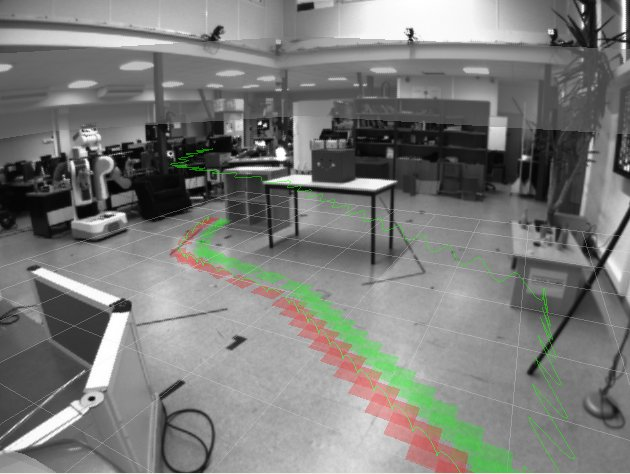
\includegraphics[width=.95\linewidth]{src/chap4-integration/footsteps2.jpg}
  \end{center}
  \caption{Affichage de la pile de pas que le robot va réaliser en
    réalité augmentée.}
\end{figure}



\paragraph{Vision stéréoscopique}\index{vision stéréoscopique}


Le dernier traitement concernait la vision monoculaire. Il est
courant, en robotique, d'avoir recours à la vision stéréoscopique afin
de pouvoir reconstruire la profondeur d'un objet visible dans les deux
caméras. Il est alors nécessaire d'estimer la transformation relative
entre les deux caméras afin de pouvoir rectifier l'image de la seconde
image de la paire de caméras stéréo. Via ce processus, les images de
deux caméras sont prises par des capteurs virtuels dans les plans
images sont coplanaires. On peut alors faire en sorte que la
projection d'un point 3d se fasse sur la même ligne tant sur la caméra
de gauche que sur la caméra de droite. Le problème de l'appariement
des points se ramène alors à un problème unidimensionnel de complexité
moindre permettant la construction d'une carte de profondeur. Cette
carte est disponible sous la forme d'un topic, mais les données de
profondeur sont également disponibles sous la forme d'un nuage de
points. Dans ce dernier, on associe à chaque point la couleur du pixel
correspondant dans l'image. Ce topic est particulièrement utile
lorsque l'on souhaite utiliser des algorithmes de traitements de
nuages de points 3D tels que PCL -- la Point Cloud Library
--\index{PCL (Point Cloud Library)}.


Une fois de plus, la totalité du processus de vision peut fonctionner
dans un processus unique afin d'éviter les copies. Cette architecture,
également adoptée sur le robot PR2\index{PR2 (robot)} de Willow
Garage, fournit donc un compromis intéressant entre rapidité,
souplesse d'utilisation et modularité.

\begin{figure}
  \begin{center}
    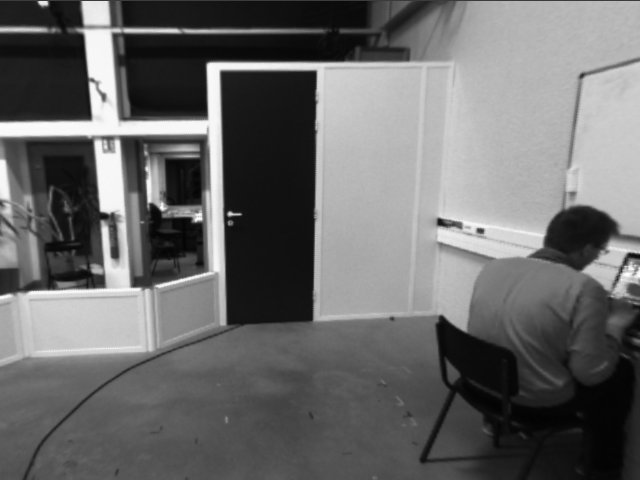
\includegraphics[width=.95\linewidth]{src/chap4-integration/disparity-1.jpg}
    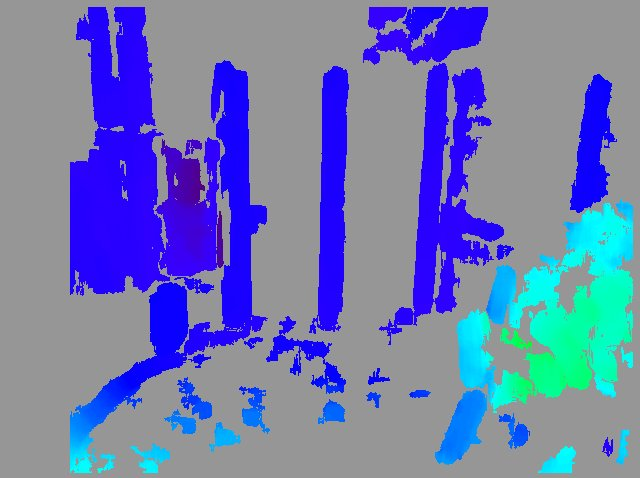
\includegraphics[width=.95\linewidth]{src/chap4-integration/disparity-2.jpg}
  \end{center}
  \caption{Carte de profondeur calculée en temps réel. Une couleur
    claire correspond à une faible profondeur, une couleur foncée à
    une profondeur importante. Les zones grises indiquent les endroits
    où aucune correspondance n'a pu être établie entre les images de
    deux caméras. Elles correspondent typiquement à une zone peu
    texturée comme un mur.}
\end{figure}


\begin{figure}
  \begin{center}
    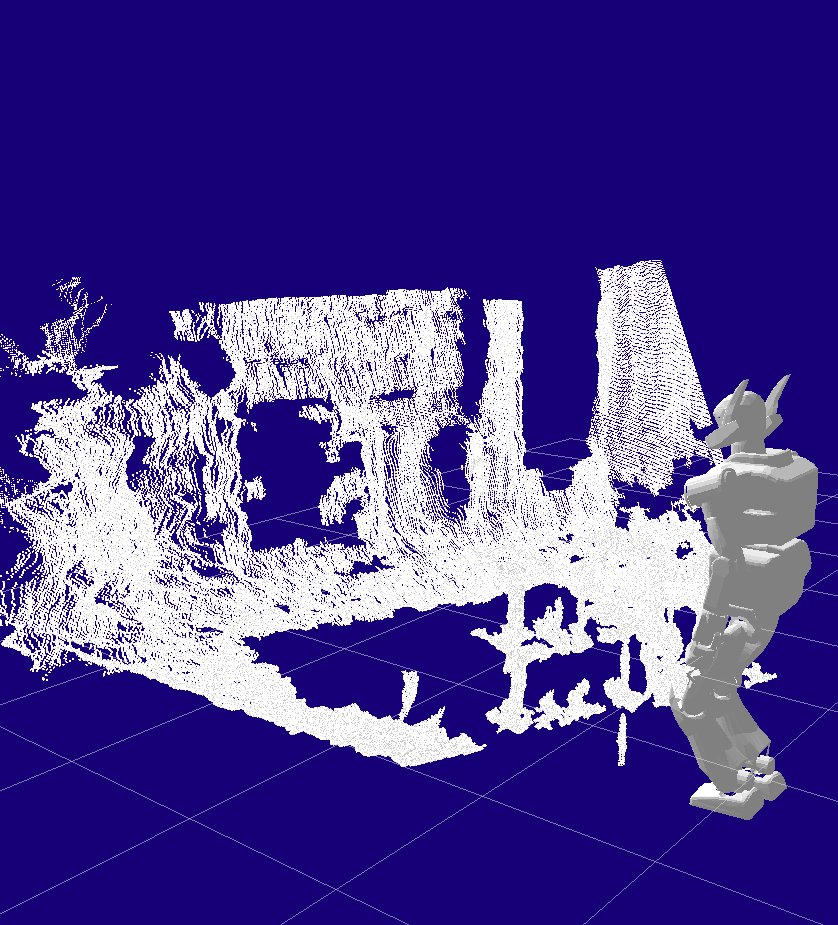
\includegraphics[width=.95\linewidth]{src/chap4-integration/stereo1.jpg}
  \end{center}
  \caption{Reconstruction 3d de l'environnement autour du robot HRP-2
    à partir des données de la paire de caméra stéréo.}
\end{figure}


\subsection{Capture de mouvement}

Une alternative à la vision embarquée est l'utilisation des systèmes
de capture de mouvement. Ces derniers, à l'origine destinés à étudier
les mouvements humains, ont été largement détournés afin de pouvoir
suivre les mouvements d'objets autour du robot et s'abstraire des
difficultés propres à la perception en robotique.


Un composant réalisant l'interface entre d'une part, le système de
capture de mouvement, et l'architecture robotique a été écrit. Ce
dernier permet de suivre les mouvements de plusieurs objets
simultanément et publie une estimation de leur pose via le système de
``topics'' précédemment décrit.


\subsection{Diagnostics et sûreté}

L'utilisation d'un robot humanoïde de grande taille présente toujours
un risque, et ce dernier tend à croître quand l'architecture devient
plus complexe et intègre des composants moins fiables. Pour se faire,
il est donc nécessaire d'avoir un moyen de pouvoir obtenir un état
complet du système de manière unifiée. Ce dernier est disponible sur
le robot et est illustré par la figure FIXME. De plus, il est
nécessaire à tout moment de pouvoir avoir un retour si le mouvement
exécuté présente le risque d'endommager le robot. Ces risques se
divisent en différentes catégories:
\begin{description}
\item[Endommagement des capteurs] Les capteurs de force sont conçus
  pour résister à un impact de 1000N au plus. Il est recommandé de ne
  pas aller au-delà de 800N par mesure de sécurité. Les autres
  capteurs ne présentent pas de risque particulier.
\item[Endommagement des actionneurs] Les actionneurs peuvent fournir
  un couple maximal. Au-delà de ce dernier, il risque de chauffer de
  manière trop importante et d'être rendu inopérant. On peut donc
  fixer une borne ``raisonnable'' qui ne devrait jamais être
  dépassée. Évidemment, ceci ne représente qu'une approximation très
  simple des capacités maximums des actionneurs. En particulier, un
  retour sur la température des actionneurs se révélerait être un
  indicateur intéressant, mais n'est malheureusement pas disponible en
  l'état actuel des capacités du robot.
\item[Instabilité lors de la locomotion] Il est possible d'estimer la
  position du ZMP à partir des forces mesurées par les capteurs de
  force. Cette estimation permet d'avertir l'utilisateur quand le ZMP
  se rapproche dangereusement de la limite du polygone de
  sustentation.
\item[Déviation des horloges des ordinateurs embarqués] Les
  ordinateurs embarqués synchronisent leurs horloges en utilisant le
  protocole NTP -- Network Time Protocol --. L'ordinateur dédié à la
  décision et la perception se synchronisent sur un serveur de temps
  distant. L'utilisation d'un lien WiFi et la présence de routeurs
  intermédiaires rendent la synchronisation relativement peu
  précise. Cependant, le problème n'est pas très gênant, car le
  véritable enjeu reste de faire en sorte que les deux PCs embarqués
  gardent leurs deux horloges synchronisées. Le lien réseau étant
  direct, la synchronisation relative de ces deux ordinateurs est, au
  contraire, de très bonne qualité et permet d'assurer la cohérence
  des données temporelles entre, d'une part, le contrôleur commandant
  les actionneurs, et d'autre part les composants de décision et de
  perception.
\item[Difficultés informatiques d'ordre général] Au-delà des problèmes
  décrits précédemment et qui affectent plus particulièrement les
  systèmes robotiques, les robots sont également affectés par
  l'ensemble des problèmes qui peuvent toucher un ordinateur:
  température excessive du processeur, manque d'espace de stockage,
  etc.
\end{description}

Une des difficultés de la mise en \oe uvre d'un système robotique est
la nécessité de faire fonctionner un ensemble de technologies
complexes sachant que le mauvais fonctionnement de n'importe quel
morceau de l'architecture peut mettre en péril la tâche tout
entière. Qui plus est, certaines limitations du matériel tel que le
couple maximum des actionneurs sont parfois vérifiées, a
posteriori. Des systèmes de surveillance des valeurs critiques sur les
couples, les impacts sur les capteurs de force ont donc été mis en
place afin d'éviter d'endommager le matériel.


\section{Simulation transparente}


Une difficulté récurrente en robotique est la lenteur de la
réalisation des expérimentations: calibrer un robot et réaliser une
expérience demande beaucoup de temps. Afin d'accélérer au maximum le
développement et d'assurer la sécurité des expérimentateurs et du
matériel, une phase de simulation des expérimentations reste cruciale.


L'utilisation d'une architecture robotique fondée sur un modèle de
communication donne ici tout son intérêt: la totalité des capacités du
matériel, tant au niveau de l'actionnement que des capteurs est
représenté informatiquement par un ensemble composé de services et de
``topics''. Tant que le simulateur choisi fournit ce même ensemble de
canaux de communication, les algorithmes pourront fonctionner
indifféremment en simulation ou sur le véritable système. Il reste
alors le plus important: assurer la cohérence entre les capteurs
simulés en fonction des commandes envoyées aux actionneurs. Pour se
faire, il est important de disposer d'un moteur physique
réaliste. Dans le cadre de cette thèse, le simulateur OpenHRP a été
choisi. En effet, la plupart des simulateurs robotiques -- Gazebo,
Webots --, utilisent des moteurs physiques primitifs adaptés aux
robots mobiles ne réalisant pas de mouvements ``dynamiques''. Afin de
modéliser précisément les interactions entre le pied et le sol, un
moteur physique disposant d'un modèle de contact convaincant et précis
est indispensable à la simulation d'un mouvement réalisé par un robot
humanoïde.


Les limitations de la plate-forme sont généralement liées à la
simulation des caméras, ne pouvant jamais reproduire les difficultés
inhérentes à la vision par ordinateur: changements d'illumination,
délai induit par l'acquisition et le transfert des données, erreur de
calibration de la caméra, etc. La simulation est donc davantage un
moyen de tester la correction du raisonnement et pas tant un outil
fiable pour démontrer sa robustesse à la réalité qui diverge toujours
du modèle calculé.


\section{Modélisation unifiée d'un système robotique}


La génération de mouvement se fonde sur une connaissance précise des
capacités physiques des robots. Cette description est généralement
encodée à l'aide d'un format de fichier permettant de représenter les
différentes informations caractérisant le système. Une définition
mathématique du système a été donnée dans le \autoref{chap:suivi}. Du
point de vue informatique, le format de fichier URDF -- Unified Robot
Description Format --, SRDF -- Semantic Robot Description Format -- et
RCPDF -- Robot Contact Point Definition Format -- est utilisé pour
représenter les informations nécessaires à la génération de mouvements
sur un robot humanoïde. Les deux premiers formats sont le fruit du
travail de la communauté ROS tandis que le dernier a été développé
dans le cadre de cette thèse.

\begin{figure}
  \begin{center}
    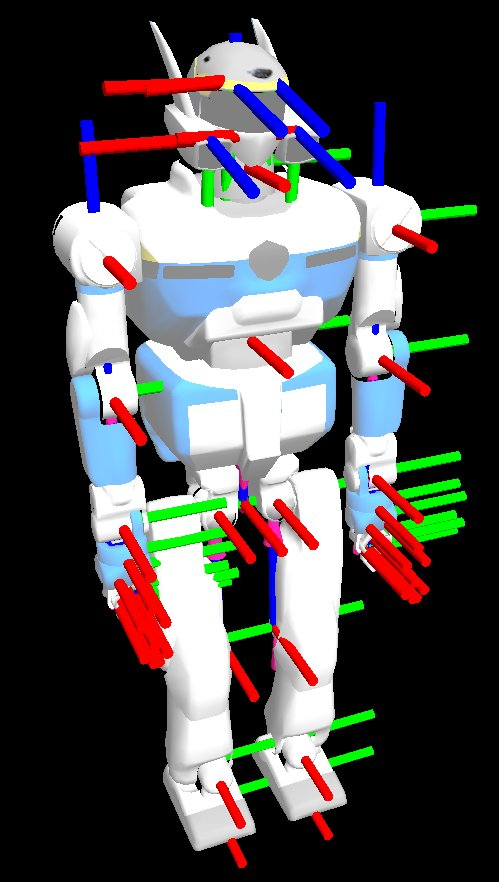
\includegraphics[width=.45\linewidth]{src/chap4-integration/hrp2_urdf.jpg}
  \end{center}
  \caption{Modèle de robot HRP-2 décrit via le format URDF.}
\end{figure}



\subsection{Description d'un robot}


Un robot est un ensemble de corps dont les mouvements relatifs sont
contraints. La modélisation des contraintes passe par la modélisation
des articulations reliant deux corps entre eux. Le format URDF définit
donc deux grands types d'objets: les corps et les joints. Nous allons
voir quelles informations sont attachées à chaque type d'objet.

\paragraph{Corps}

Un corps est défini par une forme géométrique. Cette forme peut soit
être définie par une primitive géométrique commune -- sphère,
cylindre, boîte -- ou bien via un modèle 3D. Les informations de la
dynamique du corps sont également encodées: position du centre de
masse au sein de l'objet ainsi que la matrice d'inertie associée au
corps. Une représentation alternative de la géométrie du corps
utilisée pour les calculs des collisions peut également être
définie. Dans le cas d'HRP-2, une version alternative des modèles des
corps utilisant une approximation convexe contenant moins de triangles
est disponible afin de pouvoir accélérer l'évaluation des
collisions. Une version alternative fondée sur l'utilisation de
capsules est également utilisée dans FIXME.


\paragraph{Joints}

Un joint lie deux corps tout en imposant un ensemble de contraintes au
mouvement relatif de ces deux éléments. Un joint comporte donc un lien
vers le corps ``père'' et le corps ``fils'' pour définir sa position
dans l'arbre cinématique. Dans le cas du joint racine, il peut ne pas
y avoir de corps ``père'' et dans le cas d'un organe terminal, il peut
ne pas y avoir de corps ``fils''.

Les joints supportés sont les suivants:
\begin{description}
\item[Libre] Ce joint virtuel possède six degrés de liberté et
  n'impose aucune contrainte.
\item[Rotation] Ce joint possède un degré de liberté unique et impose
  un mouvement de rotation autour d'un axe spécifique au joint.
\item[Translation] Ce joint possède un degré de liberté unique et
  impose un mouvement de translation le long d'un axe spécifique au
  joint.
\item[Planaire] Ce joint possède deux degrés de liberté et impose un
  mouvement coplanaire à un plan spécifique au joint.
\item[Fixe] Ce joint ne possède pas de degré de liberté et impose un
  mouvement rigide entre les deux corps.
\end{description}

Les degrés de liberté des joints possèdent généralement un minimum et
maximum qui sont soit le résultat de la conception mécanique du joint,
soit lié à la géométrie du robot: une valeur différente entraînerait
immédiatement une autocollision et il n'est donc pas intéressant de
considérer ces valeurs. Chaque joint comporte donc ces valeurs ainsi
qu'une vitesse et une force ou un couple maximum selon le type de
joint. Enfin la friction statique du joint ainsi que l'amortissement
utilisé pour la simulation de ce dernier peuvent également être
enregistrés.


\paragraph{Capteurs}

Une fois l'arbre cinématique défini et annoté par les corps du robot
auquel ils sont attachés, il reste encore un élément clé à spécifier:
la position des capteurs. Pour ce faire, des joints fixes définissent
la position de corps ``virtuels'' sans géométrie permettant de
spécifier la position de points importants du robot tels les capteurs.

Il n'y a malheureusement pas de description générique de ces derniers
qui permettrait de ne pas abuser de la structure cinématique du robot.


\subsection{Modélisation des préhenseurs du robot HRP-2}

La complexité du processus de génération de mouvements pour un système
croît avec le nombre de degrés de liberté. Par exemple, HRP-2 est un
système possédant 40 degrés de liberté, dont 10 pour les
mains. Cependant, tous ces degrés de liberté ne sont pas
commandables. En effet, chaque main n'est commandée que par un seul
degré de liberté décrivant le niveau de fermeture de la pince. Ces
mécanismes sont régulièrement utilisés dans les robots. On peut
également citer le robot Romeo d'Aldebaran Robotics FIXME qui s'appuie
sur un mécanisme de commande similaire: un degré de liberté commande
l'actionnement d'une main complète composé de plusieurs degrés de
liberté. Pour modéliser un tel système, il est possible d'insérer des
contraintes et des degrés de liberté ``dépendants'' dans le modèle. On
peut ainsi insérer une contrainte qui va lier deux degrés
ensemble. Par exemple dans la définition du joint A, on peut spécifier
que la valeur du degré de liberté associé dépend de la valeur du degré
de liberté du joint B:

\begin{equation}
  \mathbf{X}_B = \alpha_B \mathbf{X}_A + \beta_B
\end{equation}

Dans l'équation précédente, $\alpha_B$ et $\beta_B$ sont des
constantes propres au joint B. $\mathbf{X}_A$ et $\mathbf{X}_B$ la
valeur du degré de liberté associé respectivement aux joints A et B.


\subsection{Prise en charge des autocollisions}

Une autocollision consiste en la collision de deux corps du
robot. C'est particulièrement facile sur un humanoïde: les bras et les
jambes formant quatre chaînes distinctes pouvant entrer en collision
les unes avec les autres. D'autres cas sont également possibles: par
exemple la jambe de certains robots HRP-2 peut entrer en collision
avec le bassin dans certaines configurations. De manière générale,
toute collision qui requiert le mouvement de plusieurs degrés de
liberté combinés et qui ne peut donc pas être évitée en spécifiant les
bornes des degrés de liberté est une autocollision qui doit être prise
en compte.

Pour déterminer les autocollisions, deux stratégies sont
possibles. L'approche automatique consiste à échantillonner l'espace
des configurations du robot afin de trouver les corps qui sont soit
toujours en collision soit jamais en collision. Dans ces deux cas, la
paire de collision est rejetée. Toutes les autres sont ajoutées.  La
seconde stratégie consiste à forger la liste à la main. Dans le cas où
les autocollisions doivent être vérifiées dans la boucle temps réel,
cette technique est souvent utilisée, car les contraintes de temps de
calcul sont trop fortes pour considérer toutes les paires. On se
concentre alors sur les cas les plus probables. En particulier,
certains cas semblent difficiles à détecter automatiquement, notamment
si pour entrer en collision avec le corps A, il faut forcément
traverser le corps B alors il est inutile de prendre en compte le
corps A lors de la vérification des autocollisions.

La liste des paires de collisions est enregistrée dans un fichier
séparé utilisant le format SRDF -- Semantics Robot Description Format
--. Ce fichier stocke également la position de référence du robot dans
lequel il se situe lors du démarrage des expérimentations.


\subsection{Définition des contacts autorisés}

Un défi ouvert pour la robotique humanoïde dans les prochaines années
est la réalisation de mouvements asservis sur des sols non plans ou
utilisant des contacts avec d'autres zones du corps que les
pieds. Pour un robot donné, les contacts sont autorisés à différents
endroits, typiquement, les mains et les pieds. Il est donc nécessaire
de définir des ``zones'' où les contacts sont autorisés. Cette
information n'était pas formalisée jusqu'à présent dans l'architecture
proposée par ROS et a été le résultat d'un travail réalisé durant
cette thèse. Le format de fichier RCPDF -- Robots Contact Point
Description Format -- associe à chaque corps 0, 1 ou plusieurs zones
de contact. Chaque zone de contact peut être soit représentée par une
primitive géométrique soit par un modèle 3d. Les normales du modèles
permettent de définir la direction dans laquelle le contact peut
s'effectuer. Un contact est valide si la force de réaction de
l'environnement sur le corps du robot est colinéaire avec la normale
de la zone de contact mais de direction opposée. Enfin, la force de
réaction maximale en un point autorisée sur cette zone de contact peut
être enregistrée afin d'assurer que le contact ne va pas compromettre
l'intégrité structurelle du robot. Cette représentation offre une
formulation générique qui peut être utilisée pour réaliser des prises
de décisions moins arbitraires que celles qui sont uniquement fondées
sur l'anthropomorphisme. Par exemple, la force applicable sur les
mains du robot peut être plus contrainte ce qui peut pousser un
solveur à faire marcher le robot ``sur ses deux jambes'' sans avoir à
le lui spécifier de manière directe.

En pratique, ces données sont utilisées dans les algorithmes de marche
bipèdes et les systèmes de surveillance afin de calculer les tailles
des semelles du robot -- la zone de contact autorisée sous chaque pied
-- et, de fait, les contraintes auxquelles sont soumises le ZMP.


\subsection{Adaptation du modèle pour le contrôle et la planification}

Instrumenter le modèle pour y incorporer le maximum d'informations est
intéressant, cependant utiliser la chaîne cinématique pour positionner
des capteurs pose des problèmes pratiques. En effet, l'évaluation de
l'arbre est nécessaire pour de nombreux calculs qu'ils soient
géométriques, cinématiques ou dynamiques, inverses ou direct. La
complexité de ces algorithmes est donc dépendante de la taille de
l'arbre et la présence de joints, même fixes, pour positionner les
capteurs crée un coût supplémentaire qui semble inutile. Une
proposition est en cours pour modéliser d'une manière plus propre les
capteurs dans le format URDF, mais à l'heure actuelle il semble
intéressant de pouvoir réaliser des simplifications ou ``élagages'' de
l'arbre pour pouvoir en retirer les éléments qui ne sont pas
nécessaires. Dans le cas où les corps que l'on souhaite supprimer sont
des n\oe uds terminaux de l'arbre sans information dynamique -- comme
les capteurs --, alors l'opération peut être réalisée
directement. Cependant, dans tous les autres cas, il est nécessaire de
pouvoir calculer la masse et l'inertie équivalente de l'ensemble de
l'ensemble des corps rendus solidaires par la simplification
opérée. De fait, ces transformations de l'arbre sont un moyen bien
plus efficace d'exprimer les contraintes égalités sur certains degrés
de liberté que leur insertion en tant que contrainte dans l'algorithme
de génération de mouvement proprement dit. Les transformations
dynamiques de l'arbre sont également nécessaires pour adapter la
géométrie du robot lorsqu'il est nécessaire, par exemple, de réaliser
une tâche de locomotion en transportant un objet possédant un poids
non négligeable pouvant interférer dans la dynamique du mouvement.

Le système de représentation du robot peut d'ores et déjà encoder la
totalité des informations proposées dans cette section, mais il n'a
pas été possible, à l'heure actuelle, d'intégrer le mécanisme de
transformation de l'arbre aux logiciels de planification et de
contrôle utilisés sur le robot humanoïde HRP-2.


\section{Applications robotiques complexes}


L'ensemble des outils décrit dans la section précédente doivent être
mis en \oe uvre conjointement afin de pouvoir former une architecture
robotique cohérente. Chaque composant faisant partie d'une
architecture robotique a beau disposer d'un modèle de communication
cohérent, sembler parfaitement fonctionner pris à part et malgré tout
l'assemblage du tout reste une opération délicate: a-t-on suffisamment
de ressources pour faire fonctionner tous les composants à une vitesse
raisonnable? A-t-on une bande passante suffisamment importante entre
les ordinateurs pour communiquer les informations transmises? Le délai
de transmission perturbe-t-il l'architecture? La totalité de ces
questions ajoutées aux difficultés inhérentes au déploiement d'une
application logicielle distribuée nécessite une grande rigueur dans le
développement des démonstrations. Nous allons ici développer un
exemple de scénarii puis montrer quel bilan on peut tirer des séries
d'expériences réalisées durant cette thèse.


\subsection{Mise en place d'une application complexe}


Nous allons présenter dans cette section l'architecture de la
démonstration robotique suivante: le robot HRP-2 doit pouvoir réaliser
une tâche de locomotion pour se déplacer jusqu'à un meuble dans lequel
il souhaite déposer un objet -- dans cet exemple une balle rose
--. Pour se faire, il doit tout d'abord planifier une trajectoire
corps complet, c'est-à-dire combinant à la fois locomotion et
manipulation. Une fois cette trajectoire déterminée, il doit
l'exécuter tout en corrigeant sa trajectoire afin d'atteindre son
but. La localisation est réalisée via un système de vision fondé sur
des techniques de SLAM.

Le système est composé des composants robotiques suivant répartis sur
deux ordinateurs -- un pour le contrôle et l'autre pour la décision et
la perception --:
\begin{description}
\item[Ordinateur dédié au contrôle]
   \\
  \begin{description}
  \item[Contrôle] Ce n\oe ud est composé d'un solveur fondé sur le
    paradigme de la pile de tâches et d'une infrastructure logicielle
    utlisant le lange de programmation Python pour insérer et définir
    des tâches en cours d'exécution. Les références des tâches peuvent
    être fournies par l'extérieur via des topics. Ce composant fonctionne
    partiellement en temps réel.
  \item[Export des informations capteurs et de la
    commande\footnote{Composant remplacé lors de la simulation par un
      n\oe ud fournissant les mêmes services dans le monde
      simulé.}\addtocounter{footnote}{-1}\addtocounter{Hfootnote}{-1}]
    La commande envoyée au système, la commande après stabilisation et
    l'état actuel du robot lu sur les encodeurs est publié sous la
    forme de topics. L'accélération linéaire et la vitesse angulaire
    du torse du robot est également publié sous la forme d'un
    topic. Ce composant fonctionne partiellement en temps réel.
  \end{description}

\item[Ordinateur dédié à la décision et à la perception]
   \\
  \begin{description}
  \item[Acquisition des images\footnotemark] Capture les images venant de la paire
    stéréo grand angle.
  \item[Conversion de l'espace couleur] Transforme les images encodées
    en Bayer vers des images monochromatiques.
  \item[Rectification] Corrige la déformation de l'image liée à
    l'utilisation de l'objectif grand angle et à la conception de la
    caméra.
  \item[SLAM] Réalise une estimation de la position du robot dans le
    monde.
  \item[Cinématique directe] À partir de l'état des encodeurs, ce
    composant recalcule la position relative de tous les corps et les
    publie sous forme de topics.
  \item[Évaluation de l'erreur de positionnement] Compare la position
    voulue du robot dans le plan à un instant $t$ à la position perçue
    au même instant.
  \item[Divers] Plusieurs n\oe uds supplémentaires sont chargés de la
    surveillance des paramètres critiques du robot.
  \end{description}
\end{description}


Ces composants fournissent chacun des topics et des services qui sont
détaillés dans les figures FIXME. Les interactions entre les
composants sont détaillés dans la figure FIXME.


Cette architecture a été testée sur le robot humanoïde
HRP-2. L'architecture a fonctionné correctement, mais il n'a pas été
possible d'atteindre une précision suffisante au sein du système de
perception pour compenser avec succès la dérive du robot. En effet, le
SLAM tel que configuré ici a donné une précision de plus ou moins 5cm
ce qui est insuffisant pour des tâches de locomotions complexes. On
notera également que la phase de planification n'apparaît pas, elle a
été réalisée grâce au travail décrit dans FIXME mais sous la forme
d'une phase hors ligne. Le chemin est alors enregistré sous la forme
d'un fichier chargé au début de l'expérimentation.


\subsection{Difficultés récurrentes}

La mise en place d'une architecture modulaire pour la robotique sert
un objectif principal: contenir la complexité en assurant à
l'utilisateur la possibilité de pouvoir s'abstraire d'une partie des
traitements sous-jacents, quit à obtenir une solution
sous-optimale. En effet, l'agrégation d'outils aussi différents que la
planification de mouvement, le contrôle, l'asservissement et
différentes techniques de perception nécessite de pouvoir s'appuyer
sur des composants aussi automatiques que possible. En particulier,
concevoir des algorithmes ne nécessitant pas de paramétrage poussé est
important, mais également très difficile. Le paramétrage peut passer
soit par une phase de calibration -- comme souvent en perception --,
une phase de construction de carte, par exemple pour la navigation --
ou le réglage des stratégies adoptées par les algorithmes. Les outils
de planification nécessitent souvent le réglage de paramètres ce qui
complexifie leur utilisation. Si l'on ne peut paramétrer le système
automatiquement, il faut alors tenter de trouver un ensemble de
paramètres ayant une réalité physique qui puisse permettre à
l'utilisateur de se construire plus facilement un modèle de
comportement de l'algorithme.


Une seconde difficulté concerne l'interprétation des données. La
majorité des algorithmes produisent en sortie des données numériques,
le plus souvent avec un sens physique fort. Prenons par exemple un
composant réalisant le suivi d'un objet en temps réel: il va alors
fournir en sortie la position de l'objet dans l'espace
euclidien 3D. Une ambiguïté se pose alors: par rapport à quel repère
référence cette donnée est-elle exprimée? La caméra du robot? La
racine de sa chaîne cinématique? Un point fixe du monde? Face aux
nombreux dysfonctionnements provoqués par ce type de problème, ROS
fournit une solution clé en main: chaque transformation précise, sous
forme de chaîne de caractère, de quel repère à quel repère cette
donnée est-elle la transformation. En enregistrant ces données, on
acquiert également la possibilité de calculer automatiquement des
transformations d'un repère à un autre. Par exemple si l'on fournit la
transformation de $A$ à $B$ et de $B$ à $C$, on peut demander la
transformation de $A$ à $C$ et elle peut être calculée
automatiquement. Il y a là un véritable gain puisque l'on passe d'une
implémentation dépendant directement des données des composants auquel
on est lié vers une requête purement sémantique: ``quelle est la
position relative de la cheville gauche par rapport au poignet
droit?''. On se préserve également dans le cas où les composants
utilisés changeraient le repère de référence entre deux versions. Une
fois de plus, l'absence de typage ici rend le diagnostic difficile:
aucune erreur de compilation n'est possible et les erreurs dans les
valeurs numériques elles-mêmes sont toujours difficiles à détecter. On
notera que le système adopté ici se fonde sur le traitement des chaîne
de caractère ce qui est plus lent que le recours au typage direct tel
que proposé dans FIXME.


Une troisième difficulté est la robustesse aux phases
transitoires. Tout système complexe possède une phase d'initialisation
dans laquelle le comportement des modules peut être sous-optimal. En
particulier quand plusieurs composants communiquant ensemble sont
lancés en même temps, il n'y a aucune garantie que le premier
composant terminant sont initialisation soit toujours le même. De ce
fait, un composant peut commencer à attendre des données sur un topic
avant que le topic ne soit créé par le premier composant. Le protocole
de communication est extrêmement souple sur ce point et la possibilité
de pouvoir écouter des topics qui n'existent pas encore simplifie de
beaucoup le développement en évitant les erreurs lorsque l'ordre
d'initialisation change. Par contre, il est alors nécessaire de mettre
en place, en interne et soit même, les mécanismes afin d'éviter les
situations de famine où plusieurs composants s'attendent les uns les
autres indéfiniment. Cependant, le graphe de communication étant le
plus souvent un arbre, ce genre de cas reste peu courant.


La quatrième difficulté concerne l'initialisation du système. Il est
souvent difficile de lancer une démonstration en ``un clic'', mais
plus le nombre d'étapes pour démarrer la démonstration est important,
plus le risque d'introduire une erreur humaine lors d'une
expérimentation augmente. Il est important de limiter les opérations
pour démarrer une démonstration. Un outil utilisé dans le cadre de ce
travail est un formalisme permettant de décrire informatiquement -- en
XML\index{XML} --, le graphe formé par l'ensemble des composants
robotiques ainsi que leurs paramètres respectifs. Ce système réduit
donc au maximum les erreurs humaines, mais certaines difficultés
persistent: un robot humanoïde utilisant une commande à gains forts
telle que HRP-2 s'initialise en l'air, puis il doit être posé, le
système possède donc plusieurs phases transitoires d'initialisation
qu'il est difficile d'automatiser.


Le dernier problème récurrent est la difficulté pour un utilisateur de
déterminer si le système est dans un état stable et si ce n'est pas le
cas, arriver à diagnostiquer le système. La section précédente a
développé un ensemble d'outils permettant de surveiller l'état du
robot tant au niveau mécanique, informatique que de l'utilisation qui
en est faite en temps réel -- vérification des couples au niveau des
actionneurs notamment --. Cependant, les problèmes ne viennent pas que
de ces composants ``bas-niveau''. Des composants algorithmiques
peuvent également échouer pour diverses raisons. Pour aider la
compréhension de l'état du système, le premier élément est d'unifier
les mécanismes de rapport d'état. En effet, la plupart des
bibliothèques complexes viennent avec leur système de journalisation
qui n'est pas toujours adapté. Dans le cadre de cette architecture,
nous avons la possibilité de pouvoir agréger les informations dans un
seul topic qui peut ensuite être observé pour connaître l'évolution du
système. On a alors la liste des messages envoyés par les différents
composants dans l'ordre chronologique ce qui n'est pas le cas quand
chacun fonctionne de manière séparée. Les causes et les conséquences
sont, dans ce contexte, bien plus faciles à identifier. Le deuxième
niveau consiste à publier sur le topic de diagnostic l'état du n\oe ud.
Cela correspond à l'un des états suivants: OK, erreur,
avertissement auquel on associe des données techniques pour aider au
diagnostic. Enfin, un service standardisé peut également être fourni
par un composant pour qu'il tente un autodiagnostic. Ces mécanismes
permettent d'aider à la compréhension des erreurs.



\subsection{Bonnes pratiques pour la robotique}

Cette section détaille la méthodologie à suivre tant pour développer
un composant robotique que pour développer une architecture robotique
complète. Pour développer un composant, un exemple de développement
réalisé pendant cette thèse a été choisi: il s'agit de l'intégration
d'un logiciel de suivi. Le cycle de développement d'une architecture
robotique est ensuite détaillé.


\subsubsection{Étude de cas: intégration d'un algorithme de suivi}

Le composant dont il est question ici est librement disponible sur
internet. Il s'agit de la stack ROS
\texttt{vision\_visp}\footnote{\url{http://www.ros.org/wiki/vision_visp}}
et plus particulièrement du paquet
\texttt{visp\_tracker}\footnote{\url{http://www.ros.org/wiki/visp_tracker}}.


L'algorithme de suivi d'objet a été développé au sein de l'équipe
LAGADIC\footnote{\url{http://www.irisa.fr/lagadic/}} -- INRIA
Rennes-Bretagne Atlantique et à l'IRISA--. Cet algorithme utilise
l'asservissement visuel virtuel pour calculer une estimation de la
pose d'un objet. Le modèle de l'objet est connu et une estimation
initiale de la position de ce dernier est nécessaire. Une fois cette
estimation connue, l'algorithme tente de minimiser l'écart entre la
position des lignes -- bords -- de l'objet dans l'image par rapport à
la reprojection du modèle de l'objet suivi dans l'image. D'autres
critères que les lignes peuvent être choisis, mais c'est ce dernier
point qui a été retenu dans nos tests. La résolution de ce problème
passe par la méthode de Levenberg-Marquardt qui est proche de
l'algorithme des moindres carrés classiques.


Cet algorithme est partie intégrante de ViSP -- Visual Servoing
Platform
-- \footnote{\url{http://www.irisa.fr/lagadic/visp/visp.html}}. ViSP
intègre directement des outils pour acquérir des images à partir de
caméras ou lire des données préenregistrées, mais n'est pas un
composant robotique en lui-même.


La première étape a été de concevoir l'interface du composant: topics
et services. L'information calculée par ce programme est simple à
définir: il s'agit de la position relative de l'objet suivi par
rapport à la caméra. On peut donc ajouter un repère supplémentaire à
l'annuaire de transformations afin de spécifier la position de l'objet
suivi. Il sera dès lors possible de calculer, par exemple, la position
relative du poignet par rapport à cet objet pour tenter de
l'atteindre, s'il existe une chaîne entre de transformations entre ces
deux repères. En entrée, le problème est plus complexe. Il faut d'une
part un flux d'image, des informations de calibration, un modèle 3d de
l'objet à suivre et un jeu de paramètres permettant de régler
l'algorithme de suivi ainsi qu'une pose initiale.

\begin{figure}
  \begin{center}
    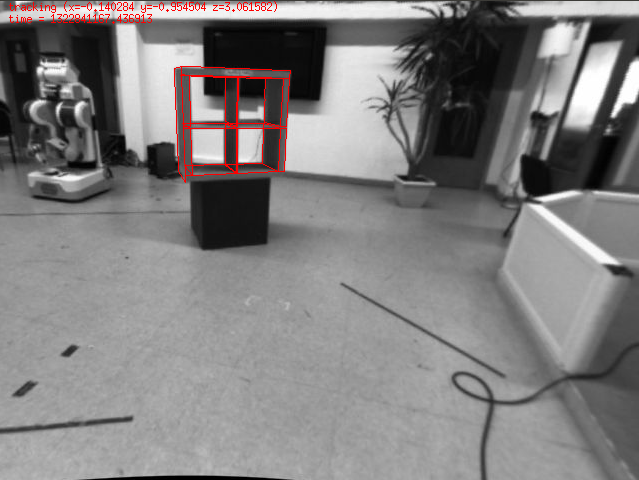
\includegraphics[width=.95\linewidth]{src/chap4-integration/shelf.png}
  \end{center}
  \caption{Le visualisateur associé au composant de suivi d'objet.}
\end{figure}



Il est courant de modéliser le comportement des composants robotiques
sous la forme d'une machine à état. Dans notre cas le composant de
suivi est dans un état ``non initialisé'' au départ où il reçoit déjà
des images et des informations de calibration, mais ne réalise aucun
traitement. Un service permet d'initialiser le suivi en fournissant à
la fois la pose initiale de l'objet, son modèle et les paramètres de
suivi. Le n\oe passse alors dans un état actif où il réalise le
suivi. Si le suivi est perdu à un moment ou un autre, le n\oe ud passe
dans un état ``perdu'' où il tente de réinitialiser le suivi avec la
dernière position connue. Si une estimation de la position de la
caméra est disponible, elle va être utilisée pour tenter de fournir
une estimation de la nouvelle position de l'objet en considérant ce
dernier statique. À n'importe quel moment le service d'initialisation
permet de relancer le suivi.


Afin de simplifier l'utilisation du n\oe ud, deux programmes
additionnels sont fournis: le premier permet de calculer une pose
initiale de manière graphique. L'utilisateur peut cliquer sur des
points de l'objet prédéfini et dont on connaît la position relative en
trois dimensions dans l'objet. Cet outil transmet également au
composant de suivi le modèle de l'objet. Le contexte distribué de
l'application empêche de passer directement des emplacements de
fichiers, car il n'y a aucune garantie que le composant réalisant le
suivi et le programme réalisant l'initialisation partage leur système
de fichier. Le modèle est donc directement transmis sous sa
représentation textuelle via le réseau. De plus, le composant pouvant
être lancé à distance, laisser l'utilisateur spécifier le chemin vers
le modèle sous la forme d'un chemin local est une mauvaise idée, car
il sera tenté d'y insérer le chemin sur sa machine et non sur celle
sur laquelle le composant va être lancé. Pour se faire, l'emplacement
du modèle est passé sous la forme d'une URI -- Uniform Resource
Identifier -- \citep{rfc2396}.


Le second outil permet de surveiller l'état du tracking en affichant
non seulement la reprojection du modèle dans l'image, mais surtout
l'état du suivi des lignes du modèle. L'algorithme pouvant rejeter des
points pour différentes raisons, cet outil fournit un retour graphique
de ces informations afin d'aider l'utilisateur à trouver le meilleur
ensemble de paramètres pour optimiser le suivi.


Le dernier point à considérer a été d'intégrer le modèle de
calibration de ROS à ViSP. En effet, ROS annote chaque image avec les
paramètres intrinsèques de caméra. Ces données sont exprimées sous
forme matricielle et doivent être converties avant d'être mises à jour
dans ViSP ce qui nécessite un traitement simple. L'avantage étant que
de cette manière, on peut complètement contourner le processus de
rectification de ViSP qui nécessiterait une calibration spécifique
pour l'utilisation de ce composant.


Les difficultés rencontrées durant cette intégration sont nombreuses:
il a fallu supprimer le code interactif, notamment pour calculer la
pose initiale qui nécessite de cliquer sur une image. Un tel code ne
peut pas fonctionner sur le robot. Il a fallu s'abstraire du système
de fichier local afin de rendre le système facilement distribuable et
il a fallu trouver une façon de pouvoir exprimer les informations de
``debug'' de manière minimale. Une solution aurait été de tracer une
image avec le résultat du suivi, mais les robots étant souvent reliés
en WiFi à la console le contrôlant, transmettre un tel flot
d'information n'est pas justifiable. À la place, un topic
supplémentaire pour les développeur a été ajouté. Le défi est alors
d'assurer la cohérence des données entre d'un côté les images
provenant du composant de vision, de la pose provenant du tracker
ainsi que du topic transportant les informations supplémentaire pour
les développeurs. Ces informations sont filtrées afin que seul les
triplets présentant un temps identique soient affichés. En effet, dans
les précédentes versions, cette synchronisation n'était pas
réalisée. On avait alors l'impression que le suivi était de mauvaise
qualité alors que le problème venait simplement de l'affichage. Les
paramètres de tracking sont également modifiables durant l'exécution
afin de simplifier la recherche du meilleur paramétrage. Cela ouvre
également la possibilité pour un composant de plus haut niveau, de
changer le comportement du logiciel de suivi et réaliser de ce fait,
une forme de suivi ``supervisé''. On notera qu'une fois de plus, la
définition des paramètres joue un rôle très important. Ici l'absence
de sens physique de certains d'entre eux est dommageable: par exemple
la recherche de la nouvelle pose se fait dans un voisinage qui est
défini en pixel. En pratique, cela signifie que si l'on se rapproche
de l'objet, l'absence de reconfiguration de ce paramètre va causer
l'échec du suivi. Un meilleur paramètre aurait été de passer par une
borne sur la vitesse maximum de la caméra qui aurait permis d'avoir un
comportement cohérent quelque soit la distance à l'objet.


Au final, ce composant a reçu un accueil favorable de la communauté
avec plusieurs utilisateurs confirmés dans des laboratoires et
sociétés tiers. Ces utilisateurs n'avaient pas d'expérience avec les
techniques d'asservissement visuel avant de tenter d'intégrer ce
composant et ont réussi à obtenir des résultats satisfaisants dans le
cadre de leur utilisation si des robots différents, notamment le robot
REEM de Pal Robotics\footnote{\url{http://www.pal-robotics.com/}}. De
ce fait l'objectif qui consistait à pouvoir maîtriser la complexité de
la mise en place d'un tel mécanisme a été rempli au travers des choix
réalisés ici. Ce composant a pu être utilisé dans le cadre d'une
architecture robotique distribuée sur deux ordinateurs et
l'introduction d'une interface au niveau de la componentisation
robotique a permis au robot HRP-2 de se localiser soit en utilisant ce
composant, soit en utilisant un composant de SLAM, soit encore le
système de capture de mouvement de manière transparente. Seul le
lancement du graphe diffère dans ces trois cas.


\subsubsection{Cycle de développement d'une architecture}


La section précédente a décrit le développement d'un composant en
particulier, mais concevoir une architecture ne revient pas à
simplement dupliquer cette approche autant de fois qu'il y a de
composants nécessaires. Il faut tout d'abord découper le problème en
composants cohérents, puis assigner ces composants à un ordinateur
parmi ceux qui équipent le robot et enfin paramétrer chacun des
composants de manière optimale. Dans la mesure où une approche
modulaire a pour intérêt principal la réutilisabilité des composants,
on sera donc contraint par l'interface des composants préexistants que
l'on devra réutiliser, ainsi que par les contraintes matérielles de la
plate-forme: les caméras d'HRP-2 sont connectées à un PC donné donc le
composant d'acquisition des images ne peut fonctionner que sur ce
dernier. Inversement, les commandes sont envoyées via une carte
connectée au second PC, le composant de contrôle ne pourra tourner que
sur celui-ci. De plus, le temps réel contraint le contrôleur a n'être
constitué que d'un seul processus. Le dernier élément à prendre en
compte est la communication intra-n\oe uds: les communications par
``topics'' ou service induisent un retard qui doit pouvoir être
accepté ou géré convenablement. Un autre élément à prendre en compte
est la bande-passante disponible entre les ordinateurs qui constituent
le robot. Il faut s'efforcer de minimiser la bande passante consommée
entre les ordinateurs. Pour les composants effectuant de l'affichage
ou de la surveillance distant le problème est souvent encore plus
critique dans la mesure où le robot est la plupart du temps connecté
en wi-fi et dispose donc d'un lien avec une bande-passante extrêmement
limitée vers l'extérieur. Cette contrainte va donc contrainte les
composants de perception, la plupart du temps gros producteurs et
consommateurs de donnée, à se situer sur le même hôte. Une fois le
traitement des images terminé, le résultat final peut représenter un
volume d'information bien plus compact: trajectoire ou position 3d par
exemple.


En considérant la répartition des composants sur les différentes
machines, il faut déterminer la liste des composants nécessaire. En
général, on part d'un côté de la liste des capteurs que l'on souhaite
utiliser, que l'on fait communiquer avec les algorithmes utilisant ces
données en entrée qui eux même communiquent avec la partie
décisionnelle. Cette partie étant généralement algorithmique, le
positionnement de ces composants n'est pas soumis à des contraintes
techniques fortes. Enfin, un composant de contrôle est nécessaire pour
envoyer les commandes.


Une fois les n\oe uds choisis et paramétrés, l'étape suivante est la
simulation. De nombreux outils permettent de simuler un mouvement
dynamique dans un monde virtuel. Il est nécessaire ici de remplacer
les composants réalisant l'acquisition des données capteurs par des
composants accédants aux informations équivalentes simulées et le
contrôleur par un contrôleur envoyant sa commande au simulateur. Une
phase supplémentaire de définition du monde est souvent nécessaire.


Une fois validée en simulation, l'architecture est portée sur le robot
proprement dit. On peut alors faire tourner l'architecture sans
envoyer réellement les commandes aux actionneurs afin de vérifier
l'accès aux données capteurs, les délais induits par les
communications entre les hôtes, etc. Enfin, l'architecture peut être
testée réellement en validant plusieurs scénarii adaptés de difficulté
croissante. Une fois l'expérience validée, on peut alors changer
certains composants afin de tester de nouvelles stratégies ce qui fait
débuter un nouveau cycle comme illustré sur la figure FIXME.


\begin{figure}
  \begin{center}
    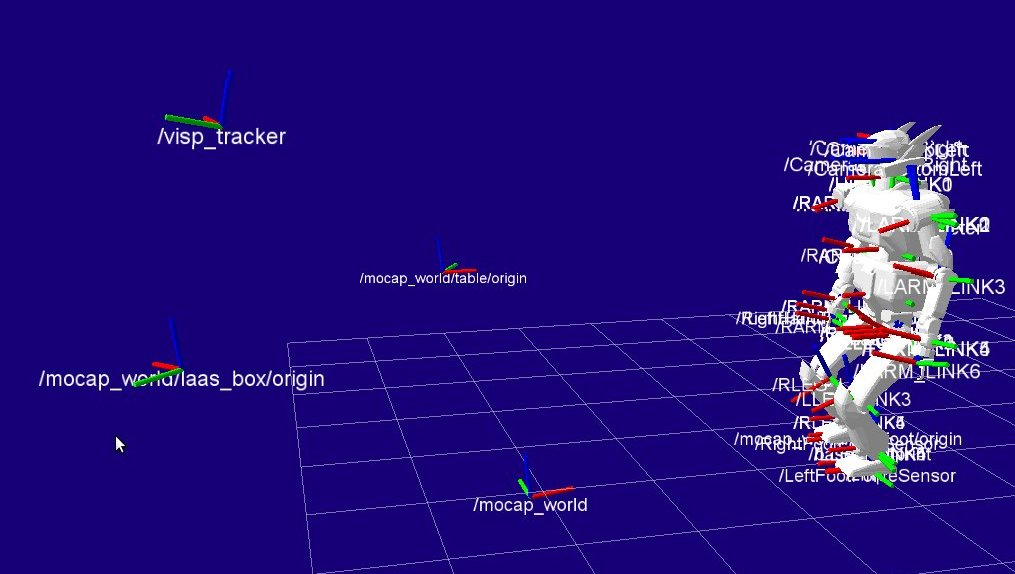
\includegraphics[width=.95\linewidth]{src/chap4-integration/rviz-full.jpg}
  \end{center}
  \caption{Architecture complexe associant de nombreux composants
    robotiques intégrant le contrôleur du robot exécutant une tâche de
    locomotion, le système de capture de mouvement et le processus
    complet de vision utilisant l'algorithme de suivi décrit dans
    cette section pour estimer la position d'un cube.}
\end{figure}



\section{Conclusion}


Construire une architecture robotique est une tâche ardue, non
seulement parce qu'elle agrège des algorithmes complexes, mais surtout
parce qu'il est nécessaire de considérer la plate-forme utilisée et
les problèmes techniques qui lui sont propres -- délais, puissance de
calcul disponible --, afin de construire un ensemble
fonctionnel. Cette section a donc à la fois présenté comment
développer un composant robotique puis comment combiner plusieurs
composants pour réaliser une architecture. Les différentes difficultés
inhérentes à la conception d'un système complexe ont été passées en
revue ainsi que les stratégies qui ont été adoptées au cours de ces
trois années. Il est probable qu'au cours des prochaines années de
nombreuses architectures robotiques complexes voient le jour sur des
robots humanoïdes afin de le rendre sensible à l'évolution de
l'environnement qui les entoure. Un objectif ambitieux pour lequel les
robots mobiles restent la plate-forme d'expérimentation principale
dans l'état actuel de la littérature.



\chapter{Conclusion}
\label{chap:conclusion}

\epigraph{\foreignlanguage{USenglish}{Can we actually "know" the
    universe? My God, it's hard enough finding your way around in
    Chinatown.}}{Woody Allen\\\emph{My Philosophy}}
\clearpage

\section{Conclusion}
\subsection{Bilan\ldots}

\lettrine[lines=2, lraise=0.1, nindent=0em, slope=-.5em]%
{L}{es} travaux présentés dans ce manuscrit de thèse ont pour but
d'améliorer les algorithmes de génération et d'exécution de mouvements
pour les robots humanoïdes. Le premier travail présenté a traité de
l'amélioration de la représentation des problèmes d'optimisation afin
de faciliter le prototypage et l'écriture de solveurs, tout en
assurant un haut niveau de sécurité. Un solveur ne doit accepter que
des problèmes qui lui sont adaptés. Une boîte à outils de fonctions de
coût et de contraintes pour l'optimisation de trajectoires a également
été conçue. L'effort théorique principal a été de chercher une
interface telle que la théorie de l'optimisation numérique se trouve
exprimée dans sa totalité tout en excluant les problèmes mal construits
et en maitrisant le coût algorithmique de la résolution des
problèmes. Par exemple, certains gradients ou hessiens peuvent ne pas
être utilisés, mais aucune approximation par différence finie ne peut
être réalisée automatiquement. C'est à l'utilisateur d'explicitement
instancier ce comportement, et d'assumer le coût de calcul
supplémentaire généré par ce type d'approche. Un tel outil est adapté
au post-traitement de trajectoires générées par des algorithmes
aléatoires notamment.

\smallskip

Le second chapitre détaille comment générer une trajectoire de marche
équilibrée sur un sol plan. Les trajectoires sont modélisées sous
forme de tâches et ces dernières sont insérées dans un solveur
temps-réel générant la commande. Le tout forme un contrôleur
polyvalent permettant, entre autres, l'exécution de trajectoires de
marche. Dans des travaux précédents, cette stratégie a déjà été
appliquée pour permettre à un robot humanoïde de marcher mais jusqu'à
présent ces tâches fonctionnaient en boucle ouverte et étaient donc
soumises à une dérive empêchant la réalisation de trajectoires longues
ou nécessitant une grande précision. L'altération du schéma de
contrôle par l'utilisation d'un composant de localisation estimant
cette dérive a permis la réalisation de mouvements d'une grande
précision. La localisation est ici prise en charge par un système de
capture de mouvements.

\smallskip

Cela nous a naturellement amenés à nous poser deux questions abordées
dans le troisième chapitre: peut-on obtenir le même résultat en
utilisant les capteurs embarqués? Peut-on représenter de manière
générique, au-delà de la simple locomotion, des trajectoires
asservies? À la première question, la réponse est, oui, il est
possible de se localiser grâce aux caméras embarquées, mais au prix
d'une précision moindre. Si cette qualité moindre ne gêne pas la
navigation en soi, elle empêche malheureusement toute manipulation
complexe une fois la trajectoire terminée. Il est donc nécessaire de
non seulement asservir la locomotion, mais également la manipulation. La
locomotion nécessite un système de localisation sans dérive, proche
des besoins d'un robot mobile alors que la manipulation nécessite avant
tout un système de localisation dont l'erreur tend vers zéro lors de
la réalisation d'un contact. Un asservissement visuel par exemple est
tout à fait adapté à cet objectif, car plus le robot s'approche de
l'objet, plus la précision croît. Malheureusement, il n'a pas été
possible de tenter une expérimentation intégrant à la fois vision
embarquée, asservissement visuel sur un objet et correction combinée
des trajectoires de locomotion et de manipulation.

\smallskip

Le dernier chapitre, quant à lui, détaille le fonctionnement de
l'architecture robotique mise en place durant cette thèse et qui a été
largement partagée avec d'autres doctorants du groupe. Il est
nécessaire de comprendre le pas franchis puisque l'on est passé d'une
architecture réalisant, soit une lecture des trajectoires articulaires
en boucle ouverte, soit la réalisation d'une pile de tâches avec un
asservissement \emph{ad hoc} dédié au scénario et difficile à
généraliser vers un système fondé sur un ensemble de composants
robotiques réutilisables. S'il n'y a pas eu écriture des composants
robotique, un travail de conception de l'architecture a été nécessaire
afin de permettre l'utilisation conjointe de toutes les capacités du
robot.



\subsection{\ldots et perspectives}


Dans le cadre du travail réalisé pour la modélisation générique des
problèmes d'optimisation, il reste encore de nombreux travaux à mener
dans trois directions différentes. La première est la représentation
informatique de fonctions mathématiques afin d'étendre l'expressivité
des fonctions. L'écriture de fonctions dépendant de plus d'une
variable se trouve compliquée par la nécessité de pouvoir calculer les
gradients combinés issus de la dérivation de plusieurs variables
différentes. La représentation d'espaces mathématiques spécifiques tel
que le groupe spécial Euclidien $\text{SE}(n)$ imposant des
contraintes tacites au solveur. La seconde direction est l'écriture de
nouvelles fonctions afin de pouvoir fournir une boîte à outils plus
complète: optimisation de posture, optimisation de trajectoires
dynamiques, ajout de critères de stabilité tel que le ZMP, etc. La
dernière direction de recherche est l'intégration de nouveaux solveurs
et de nouvelle formulations de problèmes. Par exemple, l'utilisation
du contrôle optimal est très courante en robotique. Ce domaine traite
des fonctions de coût dont la forme est très contrainte et est donc un
intéressant candidat pour être modélisé par le paradigme développé
ici.


\begin{figure}[htbp]
  \begin{center}
    \includegraphics[width=\linewidth]{src/chap5-conclusion/darpa.jpg}
  \end{center}
  \caption{Le défi DARPA pour les robots humanoïdes: les robots
    devront, entre autres, remplacer une vanne et détruire un mur pour
    pouvoir y accéder. \label{fig:darpachallenge}}
\end{figure}


Concernant le travail d'exécution de trajectoire sur robots humanoïdes,
le chemin qui reste à parcourir est clair: pour pouvoir asservir une
trajectoire automatiquement, il faut encore valider la correction des
trajectoires de manipulation, ainsi que l'utilisation d'algorithmes de
vision pour estimer la déformation nécessaire de la trajectoire des
bras. Une fois les tâches de locomotion et de manipulation asservies,
il faudra alors prendre en compte ces contraintes dans la phase de
planification. À l'heure actuelle, le planificateur peut générer un
plan de mouvement, mais il ne prend pas en compte la visibilité des
amers dans la phase de génération de la trajectoire. Il faut
privilégier les chemins assurant une qualité maximale de
l'asservissement. Les contraintes imposées par les systèmes de
localisation variant selon les cas, un dialogue entre l'étage de
planification et l'étage de perception et localisation est nécessaire.
La dernière étape serait alors de ne plus se contraindre à des
transitions temporelles dans le plan, mais également insérer des
événements logiques. Pour ce faire, il sera nécessaire d'insérer dans
l'architecture un superviseur de haut niveau permettant de réaliser la
transition entre les états logiques ainsi que de gérer les retours sur
erreur.


En conclusion, les travaux entrepris durant ces trois ans ont permis
de poser les fondations de l'exécution de trajectoires asservies sur
le robot humanoïde HRP-2, mais il reste encore un important effort à
fournir pour arriver à exécuter des scénarii longs et précis de
manière fiable. Il est fort probable que les années à venir voient
d'importants travaux dans ce sens, le prochain défi proposé par la
DARPA\index{DARPA} \citep{12darpa} étant destiné aux robots humanoïdes
-- voire \autoref{fig:darpachallenge} --. Ces derniers devront
réaliser des mouvements complexes tels que monter une échelle ou bien
encore conduire une petite voiture. Les techniques de fermeture de
boucle comme celle qui a été proposée dans ce manuscrit joueront sans
doute un grand rôle dans la réussite de scénarii de ce type.

%
%
\backmatter

\listoffigures
\listoftables

%
% Bibliography
\nocite{*}
\bibliography{thesis}
%
% Index
\cleardoublepage
\addcontentsline{toc}{chapter}{Index}
\printindex
%
\end{document}
